% Options for packages loaded elsewhere
\PassOptionsToPackage{unicode}{hyperref}
\PassOptionsToPackage{hyphens}{url}
\PassOptionsToPackage{dvipsnames,svgnames,x11names}{xcolor}
%

\documentclass[
  twocolumn]{biophys-new-mod}

\papertype{Article}


\usepackage{amsmath,amssymb}
\usepackage{lmodern}
\usepackage{iftex}
\ifPDFTeX
  \usepackage[T1]{fontenc}
  \usepackage[utf8]{inputenc}
  \usepackage{textcomp} % provide euro and other symbols
\else % if luatex or xetex
  \usepackage{unicode-math}
  \defaultfontfeatures{Scale=MatchLowercase}
  \defaultfontfeatures[\rmfamily]{Ligatures=TeX,Scale=1}
\fi
% Use upquote if available, for straight quotes in verbatim environments
\IfFileExists{upquote.sty}{\usepackage{upquote}}{}
\IfFileExists{microtype.sty}{% use microtype if available
  \usepackage[]{microtype}
  \UseMicrotypeSet[protrusion]{basicmath} % disable protrusion for tt fonts
}{}
\usepackage{xcolor}
\setlength{\emergencystretch}{3em} % prevent overfull lines
\setcounter{secnumdepth}{-\maxdimen} % remove section numbering
% Make \paragraph and \subparagraph free-standing
\ifx\paragraph\undefined\else
  \let\oldparagraph\paragraph
  \renewcommand{\paragraph}[1]{\oldparagraph{#1}\mbox{}}
\fi
\ifx\subparagraph\undefined\else
  \let\oldsubparagraph\subparagraph
  \renewcommand{\subparagraph}[1]{\oldsubparagraph{#1}\mbox{}}
\fi


\providecommand{\tightlist}{%
  \setlength{\itemsep}{0pt}\setlength{\parskip}{0pt}}\usepackage{longtable,booktabs,array}
\usepackage{calc} % for calculating minipage widths
% Correct order of tables after \paragraph or \subparagraph
\usepackage{etoolbox}
\makeatletter
\patchcmd\longtable{\par}{\if@noskipsec\mbox{}\fi\par}{}{}
\makeatother
% Allow footnotes in longtable head/foot
\IfFileExists{footnotehyper.sty}{\usepackage{footnotehyper}}{\usepackage{footnote}}
\makesavenoteenv{longtable}
\usepackage{graphicx}
\makeatletter
\def\maxwidth{\ifdim\Gin@nat@width>\linewidth\linewidth\else\Gin@nat@width\fi}
\def\maxheight{\ifdim\Gin@nat@height>\textheight\textheight\else\Gin@nat@height\fi}
\makeatother
% Scale images if necessary, so that they will not overflow the page
% margins by default, and it is still possible to overwrite the defaults
% using explicit options in \includegraphics[width, height, ...]{}
\setkeys{Gin}{width=\maxwidth,height=\maxheight,keepaspectratio}
% Set default figure placement to htbp
\makeatletter
\def\fps@figure{htbp}
\makeatother
\newlength{\cslhangindent}
\setlength{\cslhangindent}{1.5em}
\newlength{\csllabelwidth}
\setlength{\csllabelwidth}{3em}
\newlength{\cslentryspacingunit} % times entry-spacing
\setlength{\cslentryspacingunit}{\parskip}
\newenvironment{CSLReferences}[2] % #1 hanging-ident, #2 entry spacing
 {% don't indent paragraphs
  \setlength{\parindent}{0pt}
  % turn on hanging indent if param 1 is 1
  \ifodd #1
  \let\oldpar\par
  \def\par{\hangindent=\cslhangindent\oldpar}
  \fi
  % set entry spacing
  \setlength{\parskip}{#2\cslentryspacingunit}
 }%
 {}
\usepackage{calc}
\newcommand{\CSLBlock}[1]{#1\hfill\break}
\newcommand{\CSLLeftMargin}[1]{\parbox[t]{\csllabelwidth}{#1}}
\newcommand{\CSLRightInline}[1]{\parbox[t]{\linewidth - \csllabelwidth}{#1}\break}
\newcommand{\CSLIndent}[1]{\hspace{\cslhangindent}#1}

\makeatletter
\let\oldlt\longtable
\let\endoldlt\endlongtable
\def\longtable{\@ifnextchar[\longtable@i \longtable@ii}
\def\longtable@i[#1]{\begin{figure}[t]
\onecolumn
\begin{minipage}{0.5\textwidth}
\oldlt[#1]
}
\def\longtable@ii{\begin{figure}[t]
\onecolumn
\begin{minipage}{0.5\textwidth}
\oldlt
}
\def\endlongtable{\endoldlt
\end{minipage}
\twocolumn
\end{figure}}
\makeatother
\makeatletter
\@ifpackageloaded{tcolorbox}{}{\usepackage[many]{tcolorbox}}
\@ifpackageloaded{fontawesome5}{}{\usepackage{fontawesome5}}
\definecolor{quarto-callout-color}{HTML}{909090}
\definecolor{quarto-callout-note-color}{HTML}{0758E5}
\definecolor{quarto-callout-important-color}{HTML}{CC1914}
\definecolor{quarto-callout-warning-color}{HTML}{EB9113}
\definecolor{quarto-callout-tip-color}{HTML}{00A047}
\definecolor{quarto-callout-caution-color}{HTML}{FC5300}
\definecolor{quarto-callout-color-frame}{HTML}{acacac}
\definecolor{quarto-callout-note-color-frame}{HTML}{4582ec}
\definecolor{quarto-callout-important-color-frame}{HTML}{d9534f}
\definecolor{quarto-callout-warning-color-frame}{HTML}{f0ad4e}
\definecolor{quarto-callout-tip-color-frame}{HTML}{02b875}
\definecolor{quarto-callout-caution-color-frame}{HTML}{fd7e14}
\makeatother
\makeatletter
\makeatother
\makeatletter
\makeatother
\makeatletter
\@ifpackageloaded{caption}{}{\usepackage{caption}}
\AtBeginDocument{%
\ifdefined\contentsname
  \renewcommand*\contentsname{Table of contents}
\else
  \newcommand\contentsname{Table of contents}
\fi
\ifdefined\listfigurename
  \renewcommand*\listfigurename{List of Figures}
\else
  \newcommand\listfigurename{List of Figures}
\fi
\ifdefined\listtablename
  \renewcommand*\listtablename{List of Tables}
\else
  \newcommand\listtablename{List of Tables}
\fi
\ifdefined\figurename
  \renewcommand*\figurename{Figure}
\else
  \newcommand\figurename{Figure}
\fi
\ifdefined\tablename
  \renewcommand*\tablename{Table}
\else
  \newcommand\tablename{Table}
\fi
}
\@ifpackageloaded{float}{}{\usepackage{float}}
\floatstyle{ruled}
\@ifundefined{c@chapter}{\newfloat{codelisting}{h}{lop}}{\newfloat{codelisting}{h}{lop}[chapter]}
\floatname{codelisting}{Listing}
\newcommand*\listoflistings{\listof{codelisting}{List of Listings}}
\makeatother
\makeatletter
\@ifpackageloaded{caption}{}{\usepackage{caption}}
\@ifpackageloaded{subcaption}{}{\usepackage{subcaption}}
\makeatother
\makeatletter
\@ifpackageloaded{tcolorbox}{}{\usepackage[many]{tcolorbox}}
\makeatother
\makeatletter
\@ifundefined{shadecolor}{\definecolor{shadecolor}{rgb}{.97, .97, .97}}
\makeatother
\makeatletter
\makeatother
\ifLuaTeX
  \usepackage{selnolig}  % disable illegal ligatures
\fi
\IfFileExists{bookmark.sty}{\usepackage{bookmark}}{\usepackage{hyperref}}
\IfFileExists{xurl.sty}{\usepackage{xurl}}{} % add URL line breaks if available
\urlstyle{same} % disable monospaced font for URLs
\hypersetup{
  pdftitle={Intrinsically disordered region of talin's FERM domain functions as an initial PIP2 recognition site},
  pdfauthor={Jannik Buhr; Florian Franz; Frauke Gräter},
  pdfkeywords={Molecular Dynamics, Talin, Focal
Adhesion, Mechanosensing, Disorder, IDP, IDR},
  colorlinks=true,
  linkcolor={blue},
  filecolor={Maroon},
  citecolor={Blue},
  urlcolor={Blue},
  pdfcreator={LaTeX via pandoc}}


\title{Intrinsically disordered region of talin's FERM domain functions
as an initial PIP\textsubscript{2} recognition site}
\runningtitle{Intrinsically disordered region of talin's FERM domain
functions as an initial PIP\textsubscript{2} recognition site}

  \author[1,2]
  {Jannik Buhr}
  \author[1,2]
  {Florian Franz}
  \author[1,2,*]
  {Frauke Gräter}

\affil[1]{Heidelberg Institute for Theoretical Studies}
\affil[2]{Interdisciplinary Center for Scientific Computing, Heidelberg
University}

  \corrauthor[*]{Frauke.Graeter@h-its.org}

\runningauthor{Jannik Buhr, Florian Franz, Frauke Gräter}

\begin{document}
\begin{frontmatter}

\begin{abstract}
Focal adhesions (FAs) mediate the interaction of the cytoskeleton with
the extracellular matrix (ECM) in a highly dynamic fashion. talin is a
central regulator, adaptor protein and mechano-sensor of focal adhesion
complexes. For recruitment and firm attachment at FAs, talin's
N-terminal FERM domain binds to phosphatidylinositol 4,5-bisphosphate
(PIP\textsubscript{2})-enriched membranes. A newly published
autoinhibitory structure of talin-1, where the known
PIP\textsubscript{2} interaction sites are covered up, lead us to
hypothesize that a hitherto less examined loop insertion of the FERM
domain acts as an additional and initial site of contact. We evaluated
direct interactions of talin-1 with a PIP\textsubscript{2} membrane by
means of atomistic molecular dynamics (MD) simulations. We show that
this unstructured, 33-residue-long loop strongly interacts with
PIP\textsubscript{2} and can facilitate further membrane contacts,
including the canonical PIP\textsubscript{2} interactions, by serving as
a flexible membrane anchor. Under force as present at FAs, the
extensible FERM loop ensures talin to maintain membrane contacts when
pulled away from the membrane by up to 7~nm. We identify key basic
residues of the anchor mediating the highly dynamic talin-membrane
interaction. Our results put forward an intrinsically disordered loop as
a key and highly adaptable PIP\textsubscript{2} recognition site of
talin and potentially other PIP\textsubscript{2}-binding
mechano-proteins.
\end{abstract}


\begin{sigstatement}
FERM domains are modular domains that often harbor PIP\textsubscript{2}
binding sites and serve as anchoring points to membranes. talin's FERM
domain features a peculiar long and disordered loop, the function of
which has remained fully elusive. We here show by means of atomistic
molecular dynamics simulations that the loop serves as a first
PIP\textsubscript{2} interaction site and flexible anchor to the
membrane. This provides mechanistic insight into the role of
intrinsically disordered regions in protein--membrane interactions.
\end{sigstatement}


\end{frontmatter}\ifdefined\Shaded\renewenvironment{Shaded}{\begin{tcolorbox}[boxrule=0pt, breakable, frame hidden, enhanced, interior hidden, borderline west={3pt}{0pt}{shadecolor}, sharp corners]}{\end{tcolorbox}}\fi

\hypertarget{introduction}{%
\section{Introduction}\label{introduction}}

\begin{tcolorbox}[enhanced jigsaw, breakable, bottomrule=.15mm, rightrule=.15mm, left=2mm, colbacktitle=quarto-callout-tip-color!10!white, toprule=.15mm, arc=.35mm, leftrule=.75mm, colback=white, opacitybacktitle=0.6, coltitle=black, title=\textcolor{quarto-callout-tip-color}{\faLightbulb}\hspace{0.5em}{Tip}, toptitle=1mm, opacityback=0, titlerule=0mm, bottomtitle=1mm]

This is a draft and as such subject to change. The source repository for
this manuscript lives at
\url{https://github.com/hits-mbm-dev/paper-talin-loop}. The manuscript
and poster are available in multiple formats:

\begin{itemize}
\tightlist
\item
  manuscript web/html:
  \url{https://hits-mbm-dev.github.io/paper-talin-loop/}
\item
  manuscript print/pdf:
  \url{https://hits-mbm-dev.github.io/paper-talin-loop/index.pdf}
\item
  poster web/html:
  \url{https://hits-mbm-dev.github.io/paper-talin-loop/poster.html}
\item
  poster print/pdf:
  \url{https://hits-mbm-dev.github.io/paper-talin-loop/poster.pdf}
\end{itemize}

\end{tcolorbox}

Cells critically sense the mechanics of their environment at cell
adhesion sites for a multitude of biological processes. Contact with the
extracellular matrix and surrounding cells regulates growth,
differentiation, motility and even apoptosis
(\protect\hyperlink{ref-vogelLocalForceGeometry2006}{1}--\protect\hyperlink{ref-miroshnikovaAdhesionForcesCortical2018}{4}).
The multiprotein focal adhesion complex is responsible for translating
between and integrating biochemical and mechanical signals for both
outside--in and inside--out
activation(\protect\hyperlink{ref-thamilselvanPressureActivatesColon2004}{5},
\protect\hyperlink{ref-pelletierActivationStateIntegrin1995}{6}).

At the center of the focal adhesion complex sits the adaptor protein
talin, which dynamically unfolds and refolds under force
(\protect\hyperlink{ref-yaoMechanicalResponseTalin2016}{7}). A schematic
of talin can be seen in Figure~\ref{fig-tln-schema-long}. Through
interaction with integrin tails (dark green)
(\protect\hyperlink{ref-tadokoroTalinBindingIntegrin2003}{8}), which in
turn interact with collagen fibers via their heads, it links the
extracellular matrix to the intracellular cytoskeleton by directly
interacting with actin. Talin also features specific interactions with
the membrane. Their formation, mechanical stability and role in
mechanosensing remain to be fully resolved.

Talin contains an N-terminal FERM domain (F for 4.1 protein, E for
ezrin, R for radixin and M for moesin), which is composed of the
subdomains F0 to F3 and provides a link to the cytosolic side of the
plasma membrane
(\protect\hyperlink{ref-chishtiFERMDomainUnique1998}{9}). It does so via
a conserved binding motif for phosphatidylinositol 4,5-bisphosphate
(PIP\textsubscript{2}), which is enriched at active focal adhesion sites
(\protect\hyperlink{ref-maniFERMDomainPhosphoinositide2011}{10}--\protect\hyperlink{ref-songNovelMembranedependentSwitch2012a}{12}).
The main PIP\textsubscript{2} binding sites are located in F2 and F3
(highlighted as red spheres in Figure~\ref{fig-tln-schema-long}).

Two isoforms exist of talin, talin-1 and talin-2, encoded by the
\emph{tln1} and \emph{tln2} genes. This work refers to talin-1 if not
otherwise stated. Notably, the talin-1 FERM domain differs from other
FERM proteins through the addition of the F0 subdomain, which is
connected to F1 via a charged interface, as well as an insertion in F1,
a flexible loop with helical propensity and basic residues
(\protect\hyperlink{ref-goultStructureDoubleUbiquitinlike2010}{13}).
Additionally, talin's FERM domain exists in an extended conformation, as
opposed to the cloverleaf-like conformation of other FERM proteins
(\protect\hyperlink{ref-elliottStructureTalinHead2010}{14}). F3 also has
a binding site for \(\beta\)-integrin tails
(\protect\hyperlink{ref-calderwoodTalinHeadDomain1999}{15}) and is
partly responsible for the enrichment of PIP\textsubscript{2} at the
membrane through a binding site for PIPKI\(\gamma\)
(\protect\hyperlink{ref-calderwoodTalinsKindlinsPartners2013}{16}). A
second integrin binding site is located in the rod domain 11 (R11)
(\protect\hyperlink{ref-horwitzInteractionPlasmaMembrane1986}{17}).
Talin interacts with the cytoskeleton through actin binding sites
(F2-F3, R4-R8, R13-DH)
(\protect\hyperlink{ref-mccannLWEQModuleConserved1997}{18}). The review
by Klapholz et al.
(\protect\hyperlink{ref-klapholzTalinMasterIntegrin2017}{19}) provides
an excellent overview of the many interaction sites of talin and their
central role in the focal adhesion complex.

The mechanistic role of the disordered loop in the F1 domain in the many
aspects of talin function remains elusive. Its overall positive charge
renders it a prime candidate as a PIP\textsubscript{2} binding site.
However, previous studies only identified a minor role of the loop in
PIP\textsubscript{2} binding compared to F2-F3
(\protect\hyperlink{ref-chinthalapudiInteractionTalinCell2018a}{20},
\protect\hyperlink{ref-saltelNewPIP22009}{21}). On the other hand, the
F1 loop has been shown to contribute to talin-mediated integrin
activation
(\protect\hyperlink{ref-goultStructureDoubleUbiquitinlike2010}{13}).

It was previously shown that F3 can interact with R9, which impedes
integrin activation
(\protect\hyperlink{ref-bannoSubcellularLocalizationTalin2012}{22}).
Furthermore, in a recently determined cryo-electron microscopy structure
of autoinhibited talin-1, Dedden et al.
(\protect\hyperlink{ref-deddenArchitectureTalin1Reveals2019a}{23})
showed that the rod domains R9 and R12 shield the established
PIP\textsubscript{2} binding surface and the integrin binding site in F3
(see
Figure~\ref{fig-tln-schema-autoinhib}, Figure~\ref{fig-tln-align-autoinhib}).
This beckons the question how this autoinhibition can be resolved. Song
at al.
(\protect\hyperlink{ref-songNovelMembranedependentSwitch2012a}{12})
previously investigated a fragment of talin consisting of F2-F3 and an
inhibiting rod segment and suggested a pull-push mechanism, whereby
negatively charged PIP\textsubscript{2} attracts its positively charged
binding surface on F2-F3 and simultaneously repels the negatively
charged surface of the inhibitory rod segment. However, this still
leaves open the question of how talin can establish a first contact with
the membrane and remain within a sufficient proximity for this effect to
kick in.

\begin{figure}

\begin{minipage}[t]{\linewidth}

{\centering 

\raisebox{-\height}{

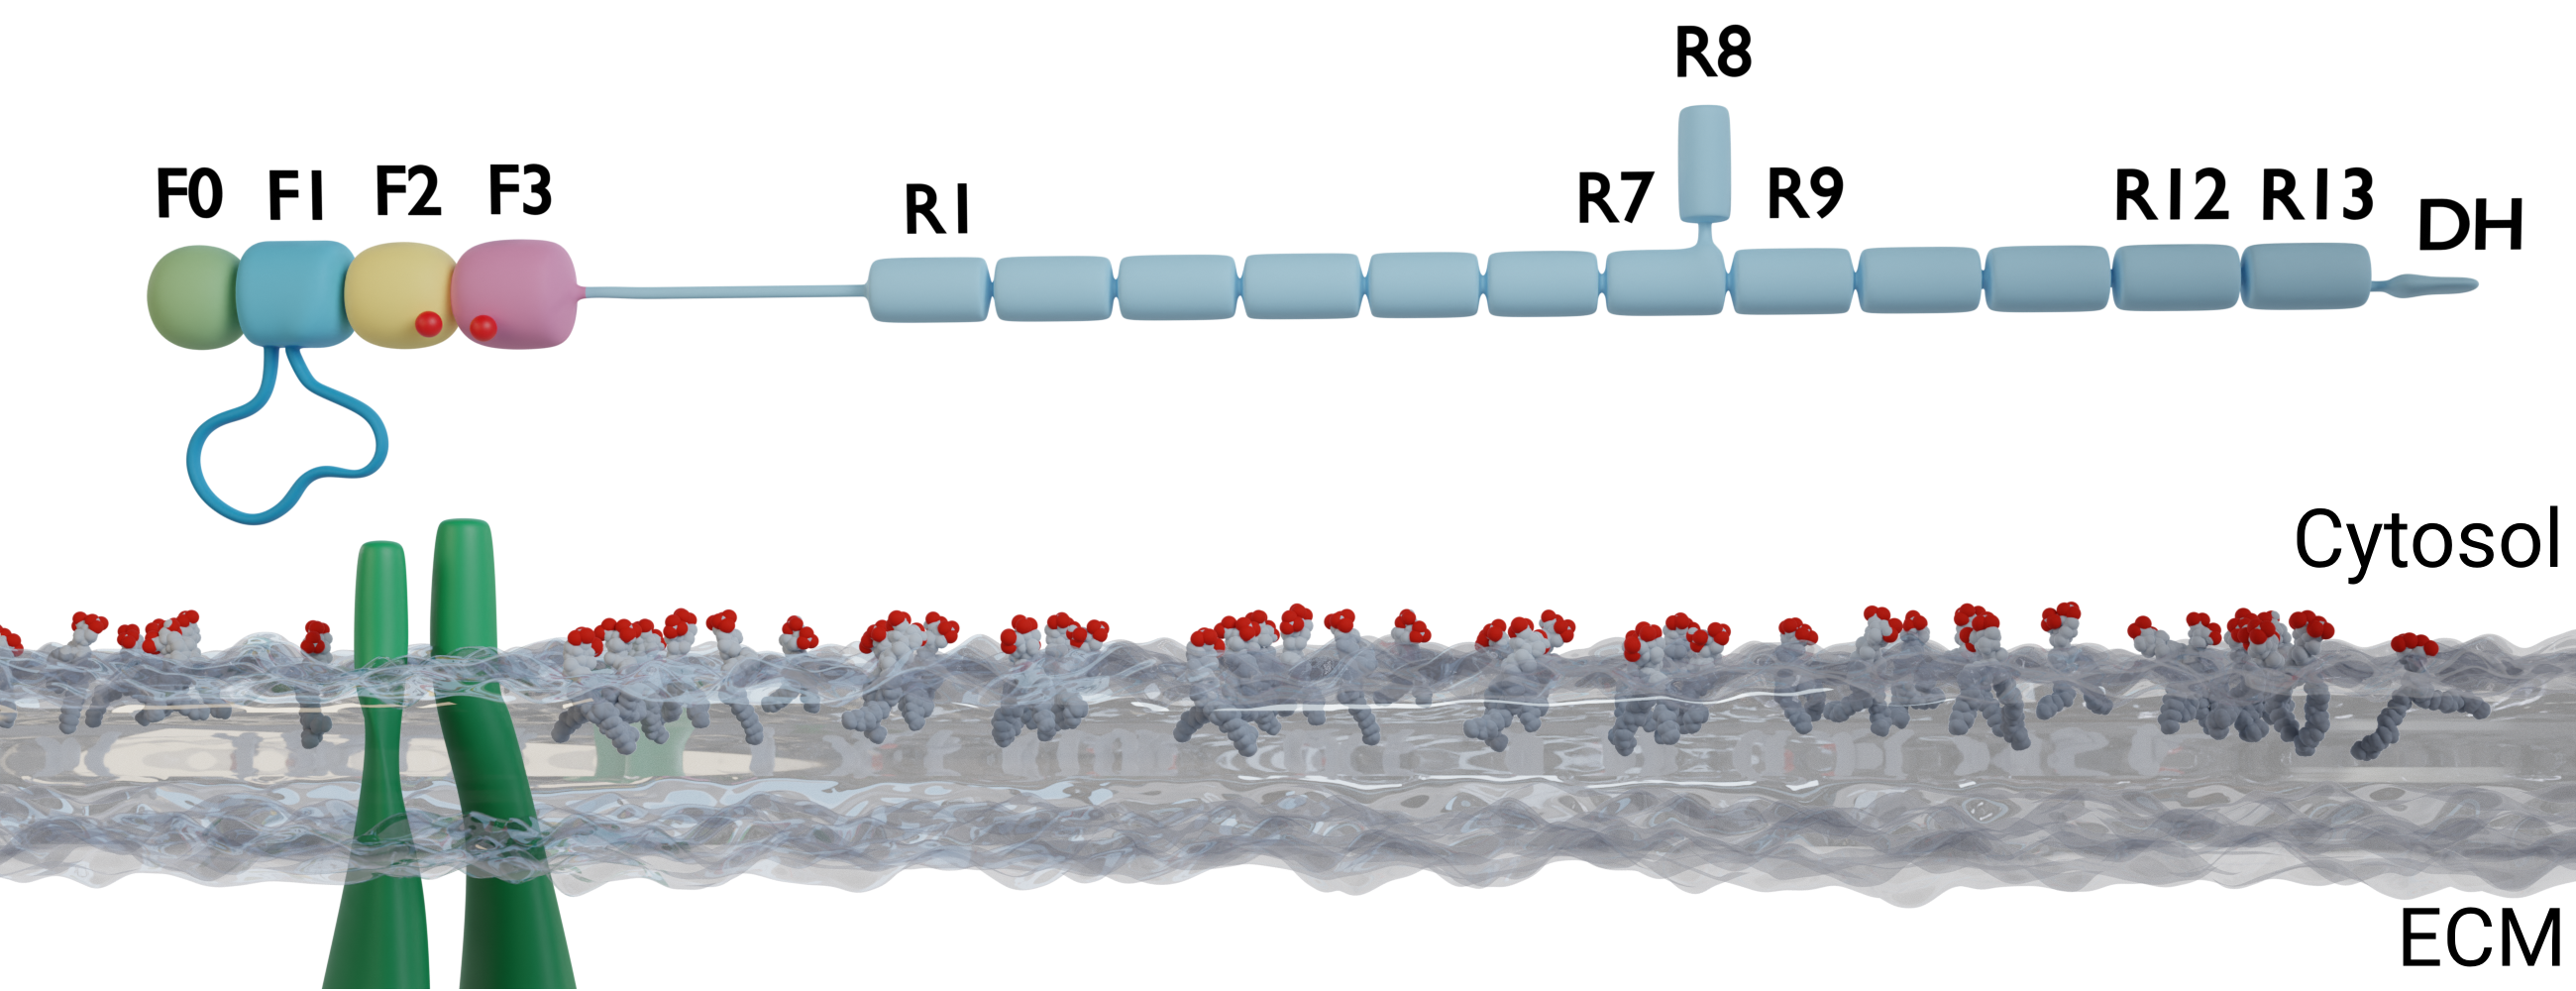
\includegraphics{./assets/blender/render/frame0000-label.png}

}

}

\subcaption{\label{fig-tln-schema-long}~}
\end{minipage}%
\newline
\begin{minipage}[t]{0.50\linewidth}

{\centering 

\raisebox{-\height}{

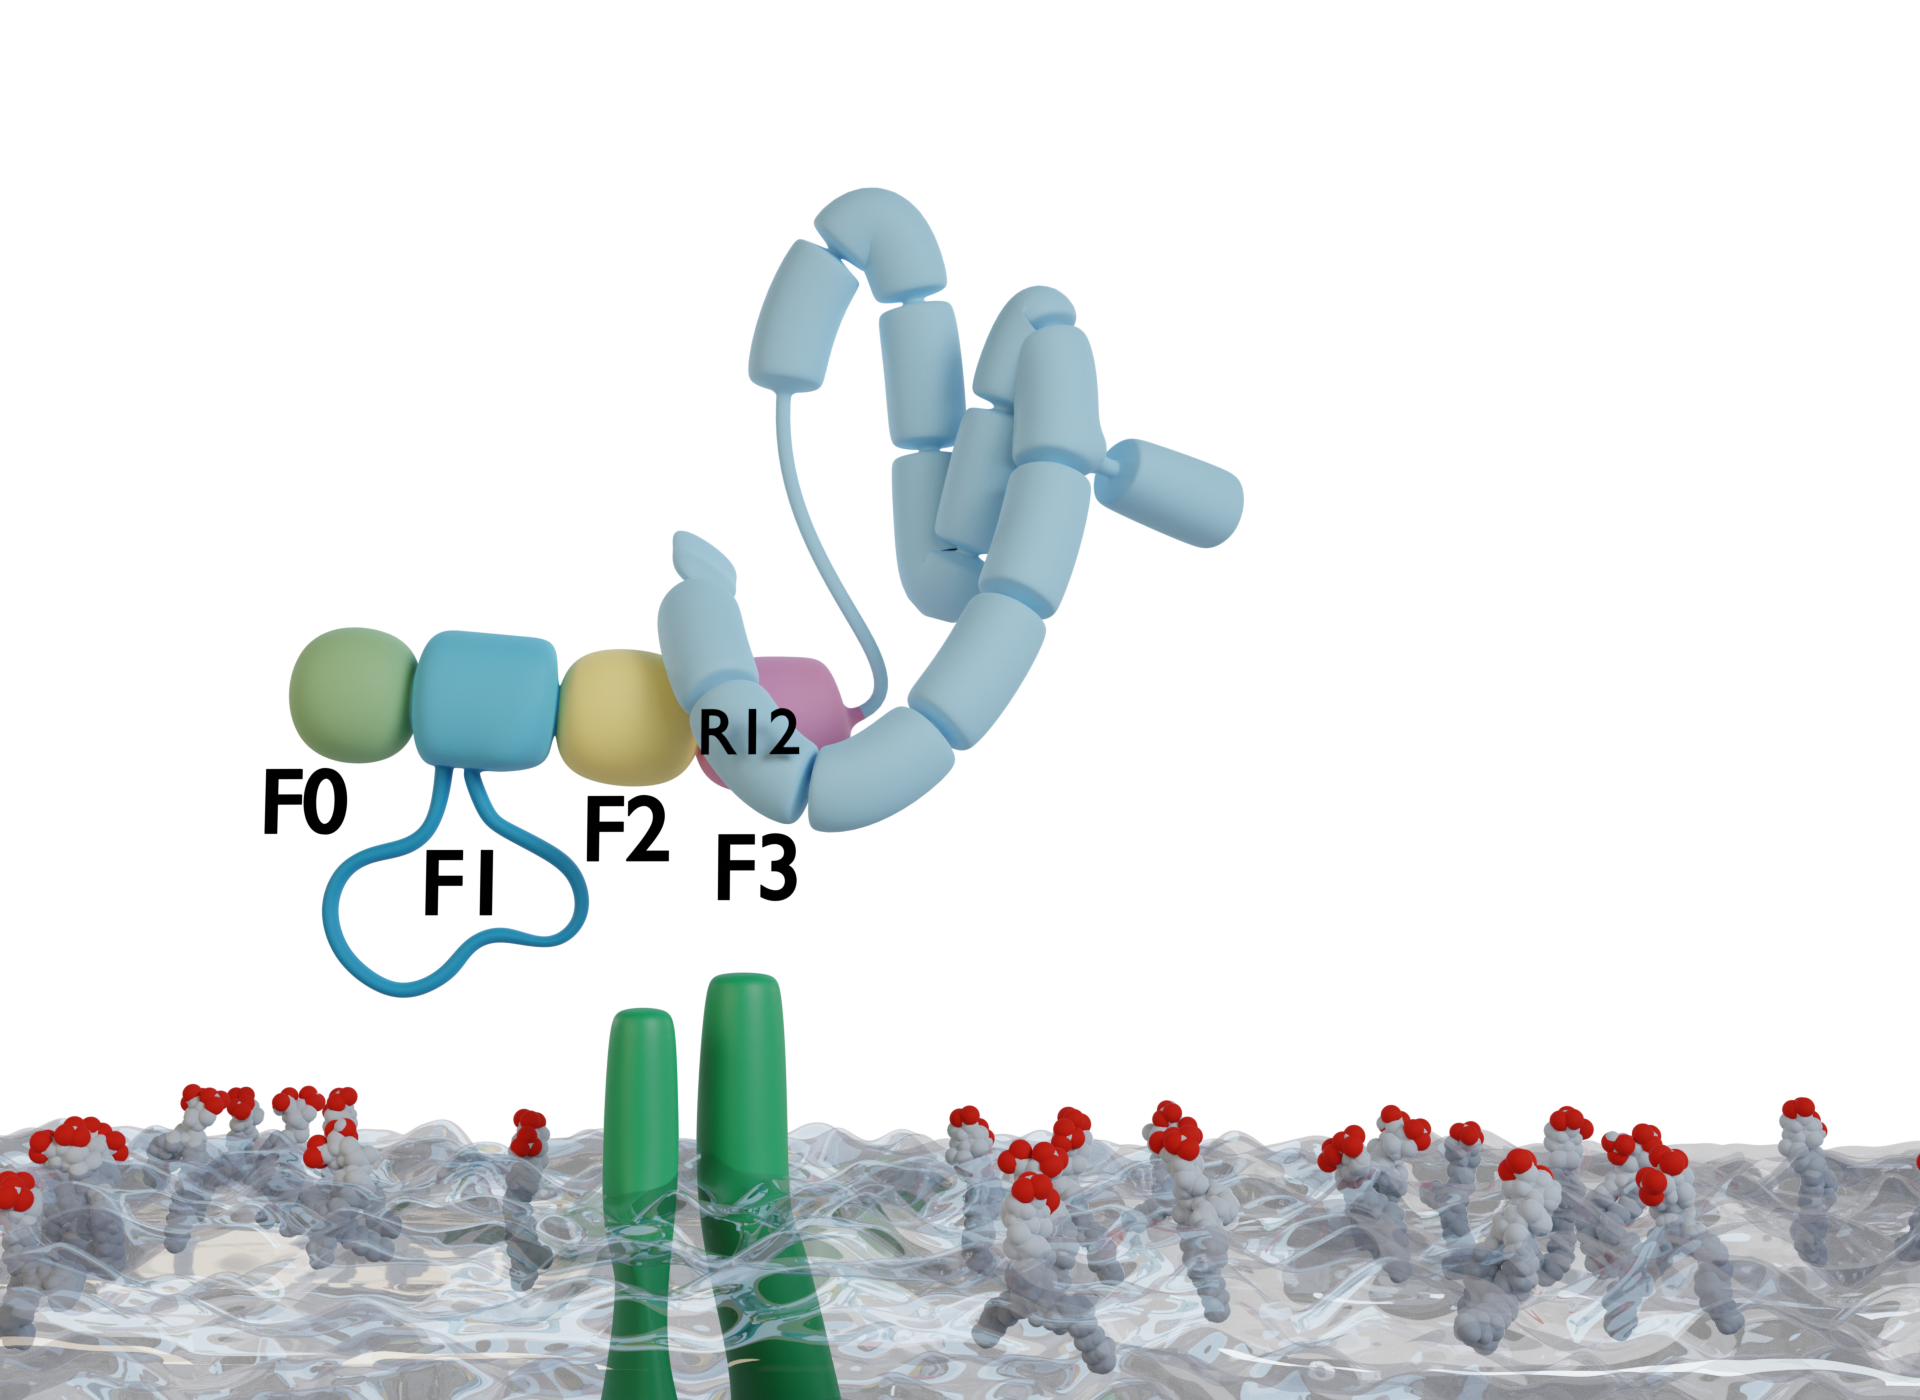
\includegraphics{./assets/blender/render/frame0001.png}

}

}

\subcaption{\label{fig-tln-schema-autoinhib}~}
\end{minipage}%
%
\begin{minipage}[t]{0.50\linewidth}

{\centering 

\raisebox{-\height}{

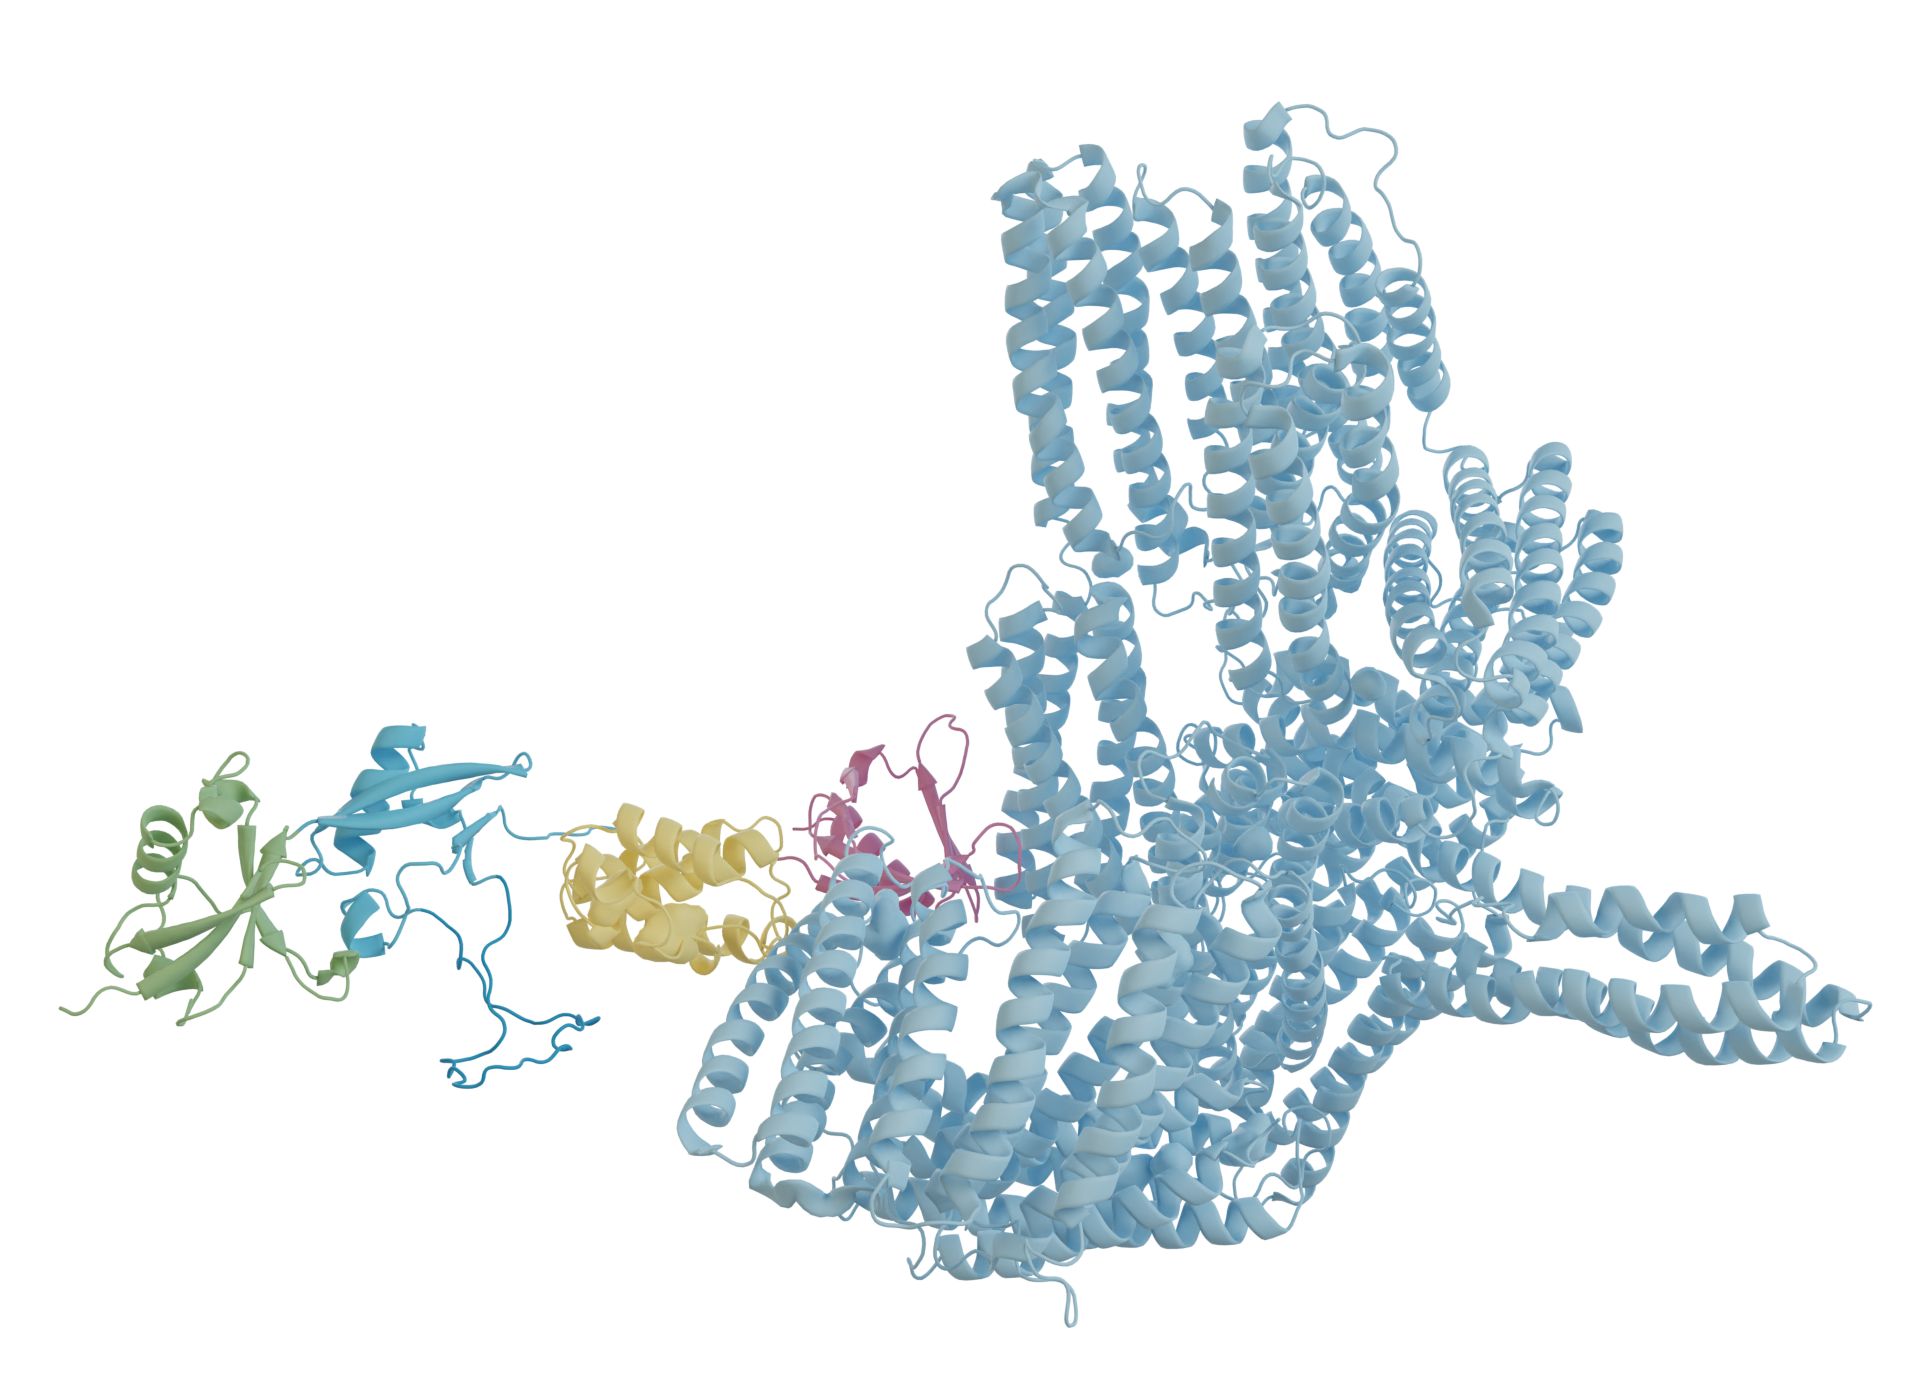
\includegraphics{./assets/blender/render-align/frame0000.png}

}

}

\subcaption{\label{fig-tln-align-autoinhib}~}
\end{minipage}%

\caption{\label{fig-structure}A schematic overview of talin and our
simulation setup. \textbf{a)} A schematic rendering of full-length talin
over a POPC membrane enriched with PIP\textsubscript{2} in the upper,
intracellular leaflet. The subdomains under scrutiny in this
publication, namely F0-F3, which comprise the N-terminal FERM domain (or
talin head), are highlighted in pastel colors (green, cyan, yellow,
magenta). The two major PIP\textsubscript{2} binding sites in F2-F3 are
marked with red spheres. The talin rod segments (or talin tail) are
numbered R1 to R13. Note that under physiological conditions, with talin
experiencing force from bound actin, the angle between the FERM domain
and the talin rod would be more akin to 30° as opposed to the linear
structure shown here for illustrative purposes. Tails of an integrin
\(\alpha\) and \(\beta\) heterodimer reaching through the lipid bilayer
are represented in green. \textbf{b)} A schematic rendering of the
autoinhibited structure of talin as crystallized by Dedden et al.
(\protect\hyperlink{ref-deddenArchitectureTalin1Reveals2019a}{23}) in
combination with a cartoon representation in \textbf{c)}. The primary
PIP\textsubscript{2} binding site of F2-F3 is occluded in talin, while
the loops of F1 is accessible, as evident when fitting the F0-F3
structure by Elliott et al.
(\protect\hyperlink{ref-elliottStructureTalinHead2010}{14}), with our
addition of the modelled F1 loop, to the autoinhibited structure, which
lacks F0F1. The main PIP\textsubscript{2}-binding sites in F2-F3 are
occluded by rod domain 12. The complete FERM structure can be explored
interactively in the context of our simulation system in the
Supplementary Materials.}

\end{figure}

We hypothesized that the flexible F1 loop inserted into talin's FERM
domain serves as an additional PIP\textsubscript{2} interaction site. As
such it would be readily accessible to PIP\textsubscript{2} even in
talin's autoinhibited conformation and would further mechanically
stabilize talin's interaction with the membrane. To test this
hypothesis, we modelled the loop, which, due to its high flexibility, is
not included in crystal structures of the FERM domain, such as PDB-ID
3IVF by Elliot et al.
(\protect\hyperlink{ref-elliottStructureTalinHead2010}{14}).

With a complete structure of the talin FERM domain, we investigated the
role of the F1 loop through atomistic molecular dynamics (MD)
simulations, which had previously also proven useful to detect the
recognition of PIP\textsubscript{2} in membranes by PH domains
(\protect\hyperlink{ref-buyanMultiscaleSimulationsSuggest2016}{24}) or
the FERM domain of focal adhesion kinase
(\protect\hyperlink{ref-zhouMechanismFocalAdhesion2015}{25}).

In F0F1 simulations, we found the loop to have a clear propensity to
interact with the PIP\textsubscript{2}-containing membrane. It is able
to establish a first contact with the membrane even from unfavorable
initial orientations due to its large search volume. Furthermore, we
show with simulations of the full-length FERM domain that once the loop
has established an initial contact, it can anchor the FERM domain to the
membrane and allow the known major binding sites in F2-F3 to form.

These results provide mechanistic insight talin--PIP\textsubscript{2}
interactions and highlight the role of secondary intrinsically
disordered binding surfaces for membrane recognition.

\hypertarget{materials-and-methods}{%
\section{Materials and Methods}\label{materials-and-methods}}

\hypertarget{molecular-dynamics-with-gromacs}{%
\subsection{Molecular dynamics with
GROMACS}\label{molecular-dynamics-with-gromacs}}

MD simulations were performed with GROMACS
(\protect\hyperlink{ref-berendsenGROMACSMessagepassingParallel1995}{26},
\protect\hyperlink{ref-abrahamGROMACSHighPerformance2015}{27}) version
2020.03 (\protect\hyperlink{ref-lindahlGROMACS2020Source2020}{28}). A
crystal structure of the talin FERM domain by Elliot et al.
(\protect\hyperlink{ref-elliottStructureTalinHead2010}{14}) with the
PDB-ID 3IVF was used as the basis of all simulations.

The deleted or missing residues (134-172) belonging to the F1 domain
loop were modeled using MODELLER
(\protect\hyperlink{ref-marti-renomComparativeProteinStructure2000}{29},
\protect\hyperlink{ref-webbComparativeProteinStructure2016}{30}) via the
interface to Chimera
(\protect\hyperlink{ref-pettersenUCSFChimeraVisualization2004}{31}),
followed by equilibration with GROMACS. The resulting conformation was
compared to an NMR structure of the F1 domain (PDB-ID 2KC2) by Goult et
al. (\protect\hyperlink{ref-goultStructureDoubleUbiquitinlike2010}{13}).
The missing residue M1 was also added. The missing residues D125 and
E126 as well as I399 and L400 were not modelled, as they are far from
the region of interest (the F1-loop). This leaves us with a sequence
from residue 1 to 398 with a shift by 2 in numbering compared to the
canonical TLN1\_MOUSE talin-1 sequence (uniprot ID P26039) after residue
124. Simulations were performed with the CHARMM36 force field.
Topologies, including the membrane, were generated with the CHARMM-GUI
web app
(\protect\hyperlink{ref-brooksCHARMMBiomolecularSimulation2009}{32}--\protect\hyperlink{ref-leeCHARMMGUIInputGenerator2016}{34})
and GROMACS tools. All simulations used the TIP3P water model and were
neutralized with 0.15 mol/L of NaCl. A 6-step equilibration was
performedafter gradient descent energy minimization. This followed the
standard procedure recommended by CHARMM-GUI, where restraints on
protein and membrane atoms were gradually relieved in six steps from
1000 and 4000~kJ/mol/nm\textsuperscript{2} for the membrane and protein
atoms on time scales of 25-100~ps, followed by 5~ns of equilibration
with only protein atoms subjected to 50 kJ/mol/nm\textsuperscript{2}
position restraints. The exact Molecular Dynamics Parameter (mdp) files
are provided in the data (\url{https://doi.org/10.11588/data/BQTQUN}) in
the \texttt{assets} folder of each simulation system. Production runs
used a timestep of 2 fs, a Verlet cut-off scheme for Van-der-Waals
interactions and the Particle Mesh Ewald (PME) method for long-range
electrostatics. NPT-ensembles were achieved by Nosé-Hoover temperature
coupling
(\protect\hyperlink{ref-hooverCanonicalDynamicsEquilibrium1985}{35},
\protect\hyperlink{ref-noseUnifiedFormulationConstant1984}{36}) and
Parinello-Rahman pressure coupling
(\protect\hyperlink{ref-parrinelloPolymorphicTransitionsSingle1981}{37}).
An example \texttt{.mdp}-file can be found in the Supplementary
Materials.

The initial equilibrium simulation of the completed FERM domain was run
for 75 ns. Subsequently, the root mean squared fluctuation (RMSF) was
calculated with GROMACS tools (see Supplementary Material Figure 7a and
7b).

The F0F1 FERM sub domains (residues 1 to 197) were simulated to evaluate
protein-membrane association using a rotational sampling approach. This
entailed placing the protein 1.5~nm away from a
1-palmitoyl-2-oleoyl-glycero-3-phosphocholine (POPC) membrane, where 12
of the 119 lipids in the upper leaflet were replaced with
PIP\textsubscript{2}. This results in a physiological concentration of
10\% PIP\textsubscript{2}. The PIP\textsubscript{2} molecules used in
the simulutions have a charge of -4, consistent with the deprotonation
state of the phosphate groups at physiological pH
(\protect\hyperlink{ref-mclaughlinPIP2ProteinsInteractions2002}{38}).

60 different starting orientations of the protein where generate,
spanning a rotation of 360 degrees. The protein was rotated in such a
way that the respective closest residue had the same distance to the
membrane for the 0° and the 180° starting positions. 6 replicates of
each orientation were run for 200~ns each. However, due to a hardware
failure, 2 of these 360 runs are corrupted and thus excluded from the
analysis.

From this rotational sampling, we selected representative conformations
with loop-membrane interactions as the basis of 6 equilibrium
simulations of the complete FERM domain over a POPC membrane with 26
PIP\textsubscript{2} lipids out of a total of 273 lipids in the upper
leaflet. Each simulation ran for 400~ns. The initial conformations for
perpendicular pulling simulations of the F0F1 subdomains to gauge
interaction strength were also chose from the rotational sampling set.
The pulling simulations used an umbrella potential applied to the
C-terminus with a harmonic force constant of 500
kJ/mol/nm\textsuperscript{2} and a constant speed of 0.03 m/s (See
Supplementary Data in \texttt{f0f1-vert-pulling/pull\_00003.mdp})

Distance information was extracted from trajectories with gromacs tools
interfaced via CONAN
(\protect\hyperlink{ref-mercadanteCONANToolDecode2018}{39}).

\hypertarget{automation-data-analysis-and-availability}{%
\subsection{Automation, Data Analysis and
Availability}\label{automation-data-analysis-and-availability}}

Setup scripts written in bash are available for all simulations shown in
this work. Computations for data analysis were tracked with the targets
R package (\protect\hyperlink{ref-landauTargetsPackageDynamic2021}{40}).
Plots were generated with ggplot2 (\protect\hyperlink{ref-ggplot}{41}).
Interactive structure representations are embedded using Mol*
(\protect\hyperlink{ref-molstar}{42}). Schematic visualizations were
rendered with blender (\protect\hyperlink{ref-blender}{43}) and VMD
(\protect\hyperlink{ref-vmd}{44}). Files relevant to this work that are
too big to be uploaded to this repository are available here:
\url{https://doi.org/10.11588/data/BQTQUN}. This manuscript was
generated with \href{https://quarto.org/}{quarto}
(\protect\hyperlink{ref-quarto}{45}--\protect\hyperlink{ref-rbetterposter}{47}).

\hypertarget{results}{%
\section{Results}\label{results}}

\hypertarget{the-f1-loop-can-act-as-a-point-of-first-contact}{%
\subsection{The F1 loop can act as a point of first
contact}\label{the-f1-loop-can-act-as-a-point-of-first-contact}}

The high flexibility of the F1 loop gave use the confidence to model it
from sequence. It retained its flexibility in equilibrium simulations,
in close agreement with the conformational flexibility reflected in the
NMR ensemble of the F1 domain
(\protect\hyperlink{ref-goultStructureDoubleUbiquitinlike2010}{13}),
which confirmed this approach (see Supplementary Material Figure 7a and
Figure 9). The resulting system that provides the basis for our
simulations can be explored interactively in the Supplementary
Materials.

When simulating only F0F1 over a POPC membrane containing 10\%
PIP\textsubscript{2}, we noticed that the F1 loop had a clear propensity
to establish contact with the membrane. Once the contact had been
established, the protein was anchored strongly enough for more contacts
to evolve with time, pulling the protein onto the membrane
(Figure~\ref{fig-f0f1-snapshots}). In order to control for a potential
bias towards the loop as a result of the starting position, we performed
a rotational sampling of the system, where the starting angle of the
loop with respect to the membrane was varied across 60 equally spaced
angles. Figure~\ref{fig-f0f1-ri-angle} shows that independent of the
starting position, the loop is able to find the membrane and bind to it.
A residue of the F1 loop is likely to be the first to establish membrane
contact even in simulations where the loop starts oriented away from the
membrane (also see Supplementary Material Figure 8). This is due to the
large search space it can cover with its high flexibility (see
Supplementary Material Figure 7a). Expectedly, binding happens earlier
in the simulation when the loop starts oriented favorably towards the
membrane (Figure~\ref{fig-f0f1-angle-frame}, 0~°) and the time to first
contact is shorter for residues of the F1 loop (see Supplementary
Material). While Figure~\ref{fig-f0f1-snapshots} shows one example of a
bound conformation, a conformation for each starting angle can be seen
in the \protect\hyperlink{sec-system}{Supplementary Material}.

\begin{figure}

\begin{minipage}[t]{\linewidth}

{\centering 

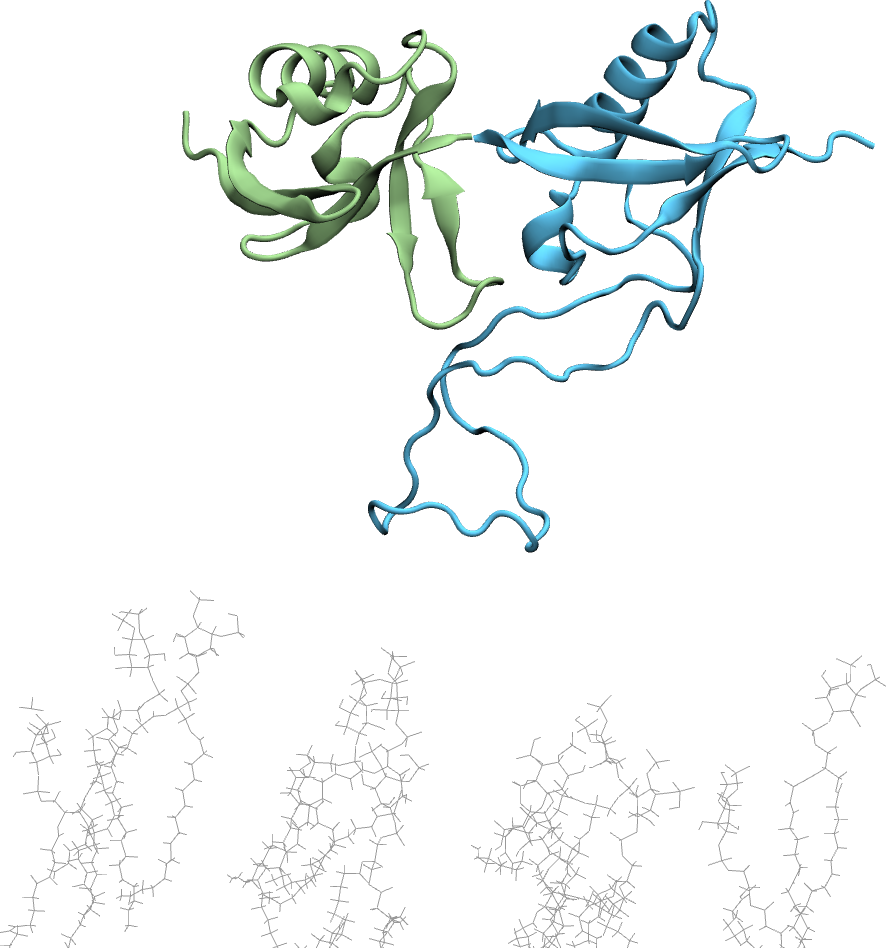
\includegraphics[width=0.3\textwidth,height=\textheight]{./assets/vmd/f0f1/unbround-trim.png}
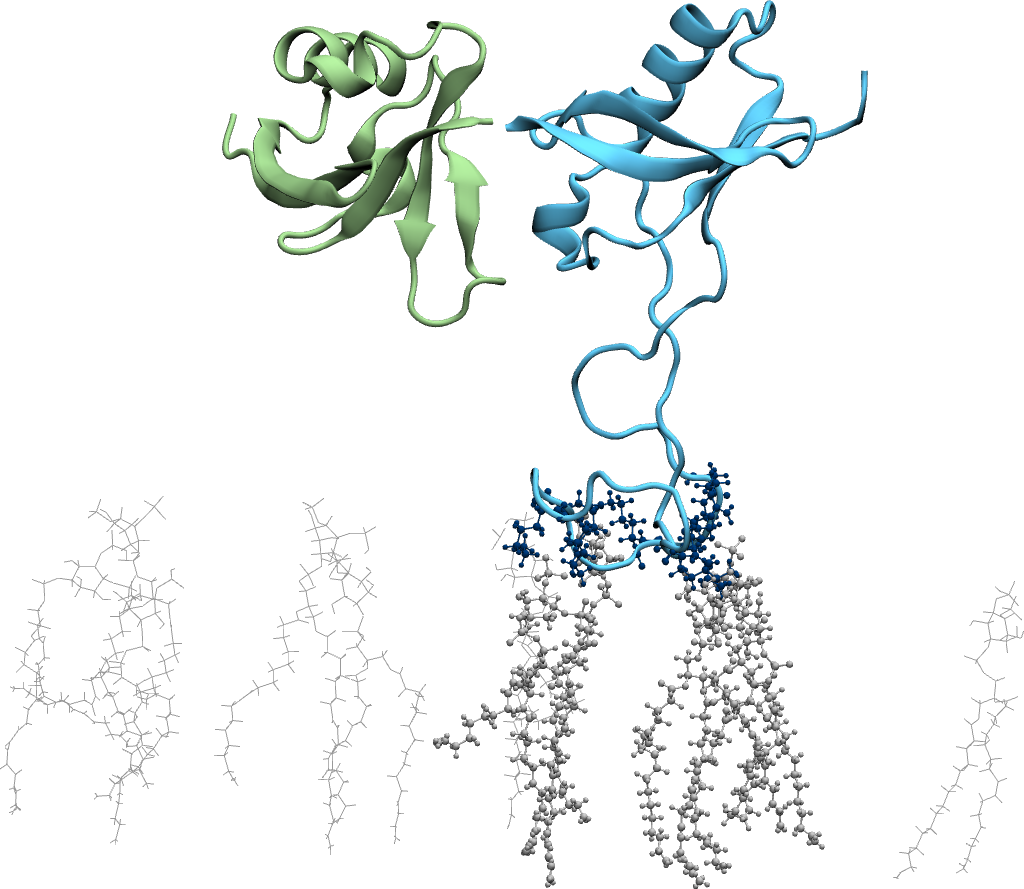
\includegraphics[width=0.3\textwidth,height=\textheight]{./assets/vmd/f0f1/anchored-trim.png}
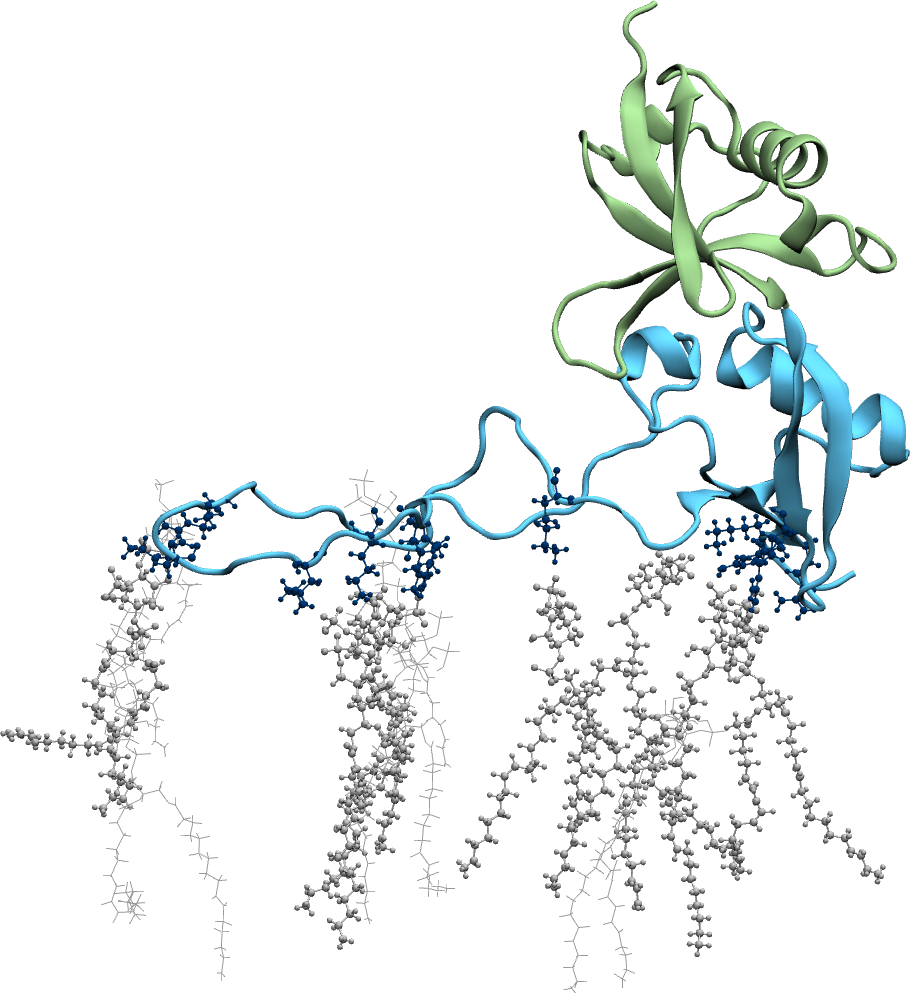
\includegraphics[width=0.3\textwidth,height=\textheight]{./assets/vmd/f0f1/bound-trim.png}

}

\subcaption{\label{fig-f0f1-snapshots}~}
\end{minipage}%
\newline
\begin{minipage}[t]{\linewidth}

{\centering 

\raisebox{-\height}{

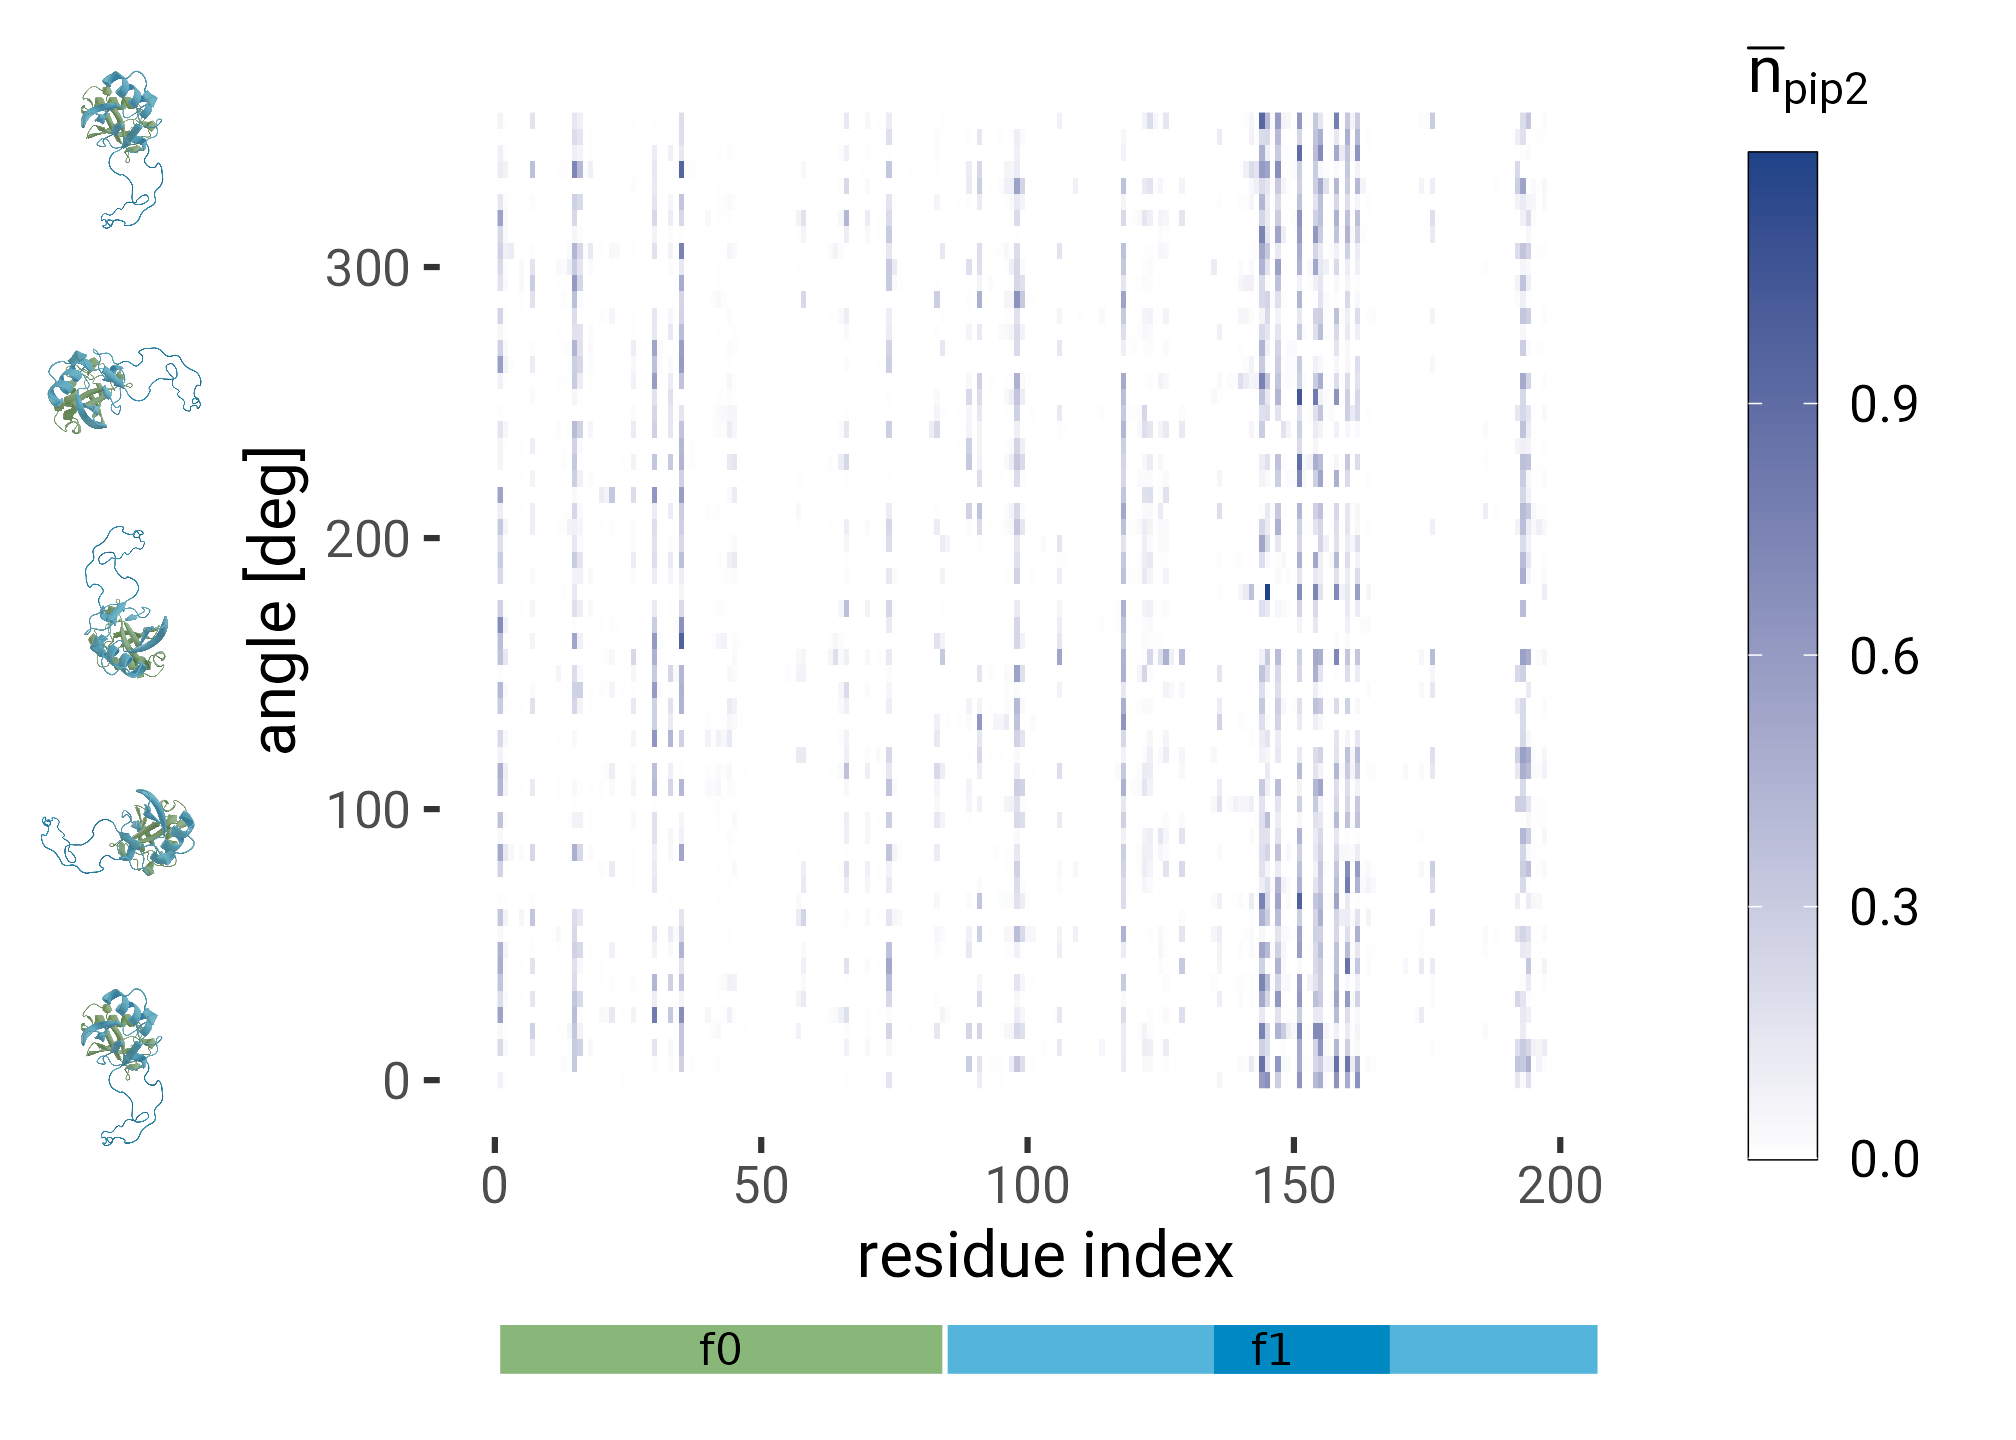
\includegraphics{./results/plots/f0f1-ri-angle-npip-1.png}

}

}

\subcaption{\label{fig-f0f1-ri-angle}~}
\end{minipage}%

\caption{\label{fig-loop-importance}Rotational sampling of F0F1 reveals
the lipid binding capabilities of the F1 loop. \textbf{a)} Snapshots
from a simulation involving F0F1 over a POPC membrane containing 10\%
PIP\textsubscript{2} in the upper leaflet. POPC is not rendered and
PIP\textsubscript{2} is shown as light grey stick models that turn
thicker for those molecules that are currently interacting with residues
of the protein. The PIP\textsubscript{2}-binding residues are then shown
as dark blue stick models. \textbf{b)} Time-averaged number of
PIP\textsubscript{2} molecules bound per residue along the F0F1 sequence
(x-axis) as a heatmap summarizing 358 simulations from a rotational
sampling, with the starting angle on the y-axis. We sampled 60 different
starting positions, rotated equally spaced around the horizontal axis,
with 6 replicates each. Each simulation is 200~ns long. 0° corresponds
to the loop pointing downwards towards the membrane, as shown in the
smaller renders to the left of the heatmap.}

\end{figure}

Once a contact has been made, it becomes exceedingly unlikely for F0F1
to dissociate from the membrane (Figure~\ref{fig-f0f1-retention}). Out
of 358 runs\footnote{6 replicas each for 60 angles minus 2 runs lost to
  a storage failure}, 89 runs never made contact with the membrane, but
out of the 269 that did, only 10 eventually dissociated. Thus, the
simulated timeframe of 200~ns per trajectory allowed for the observation
of some reversibility of FERM--PIP\textsubscript{2} binding, albeit only
for weakly bound cases and at a small rate of 3.7\%. Dissociation from
the membrane never occurred on the simulated time scale after more than
3 residues had already made contact.

\begin{figure}

\begin{minipage}[t]{\linewidth}

{\centering 

\raisebox{-\height}{

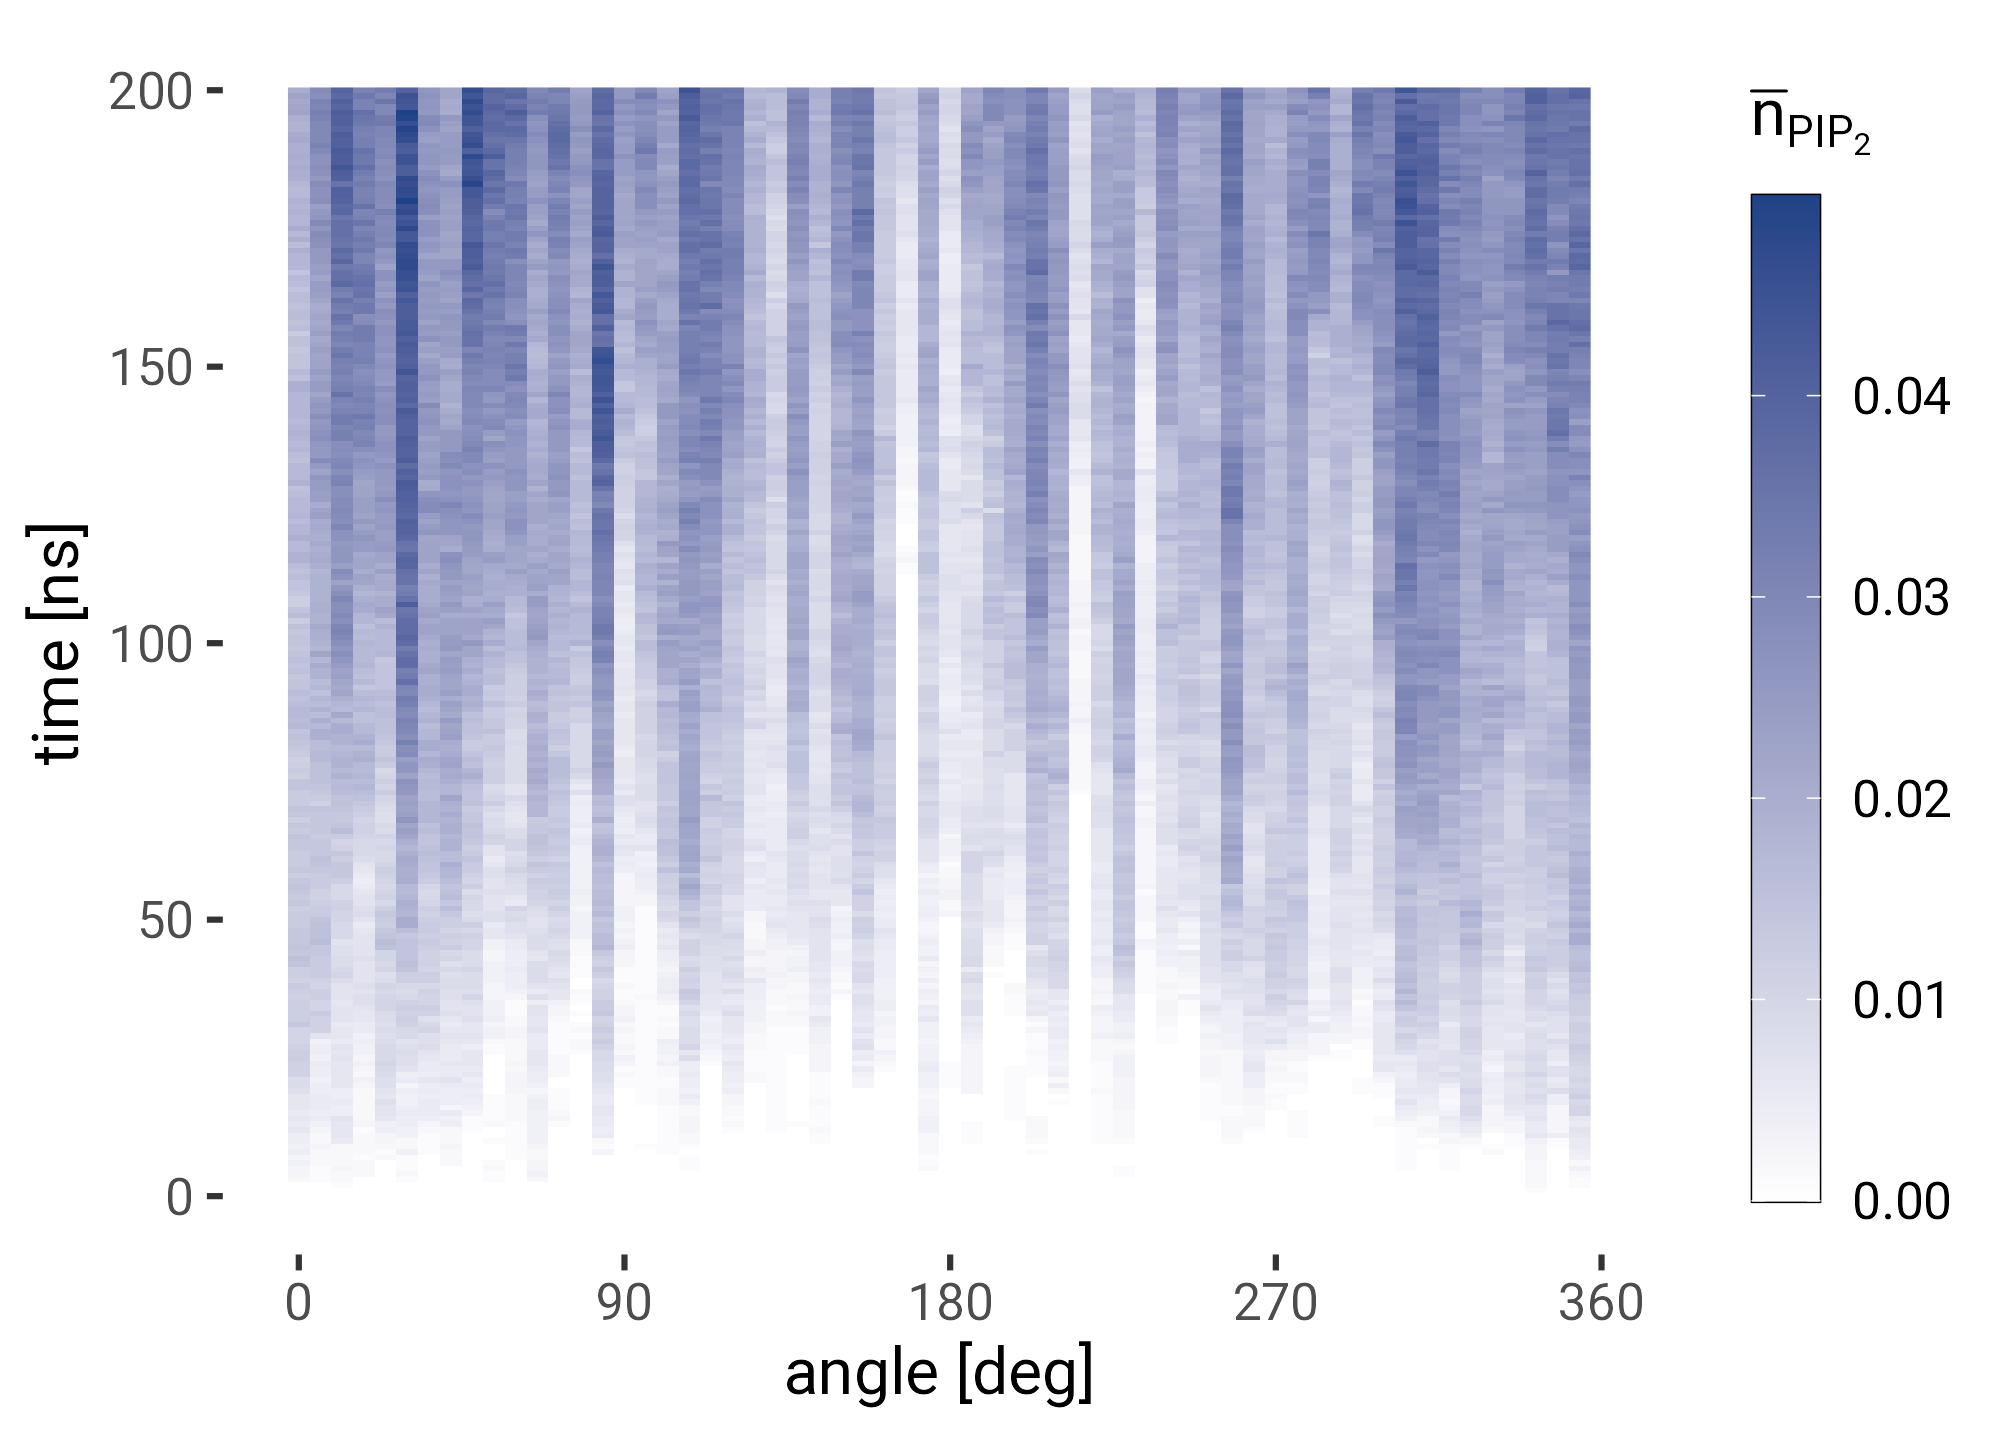
\includegraphics{./results/plots/f0f1-angle-frame-npip-1.png}

}

}

\subcaption{\label{fig-f0f1-angle-frame}~}
\end{minipage}%
\newline
\begin{minipage}[t]{\linewidth}

{\centering 

\raisebox{-\height}{

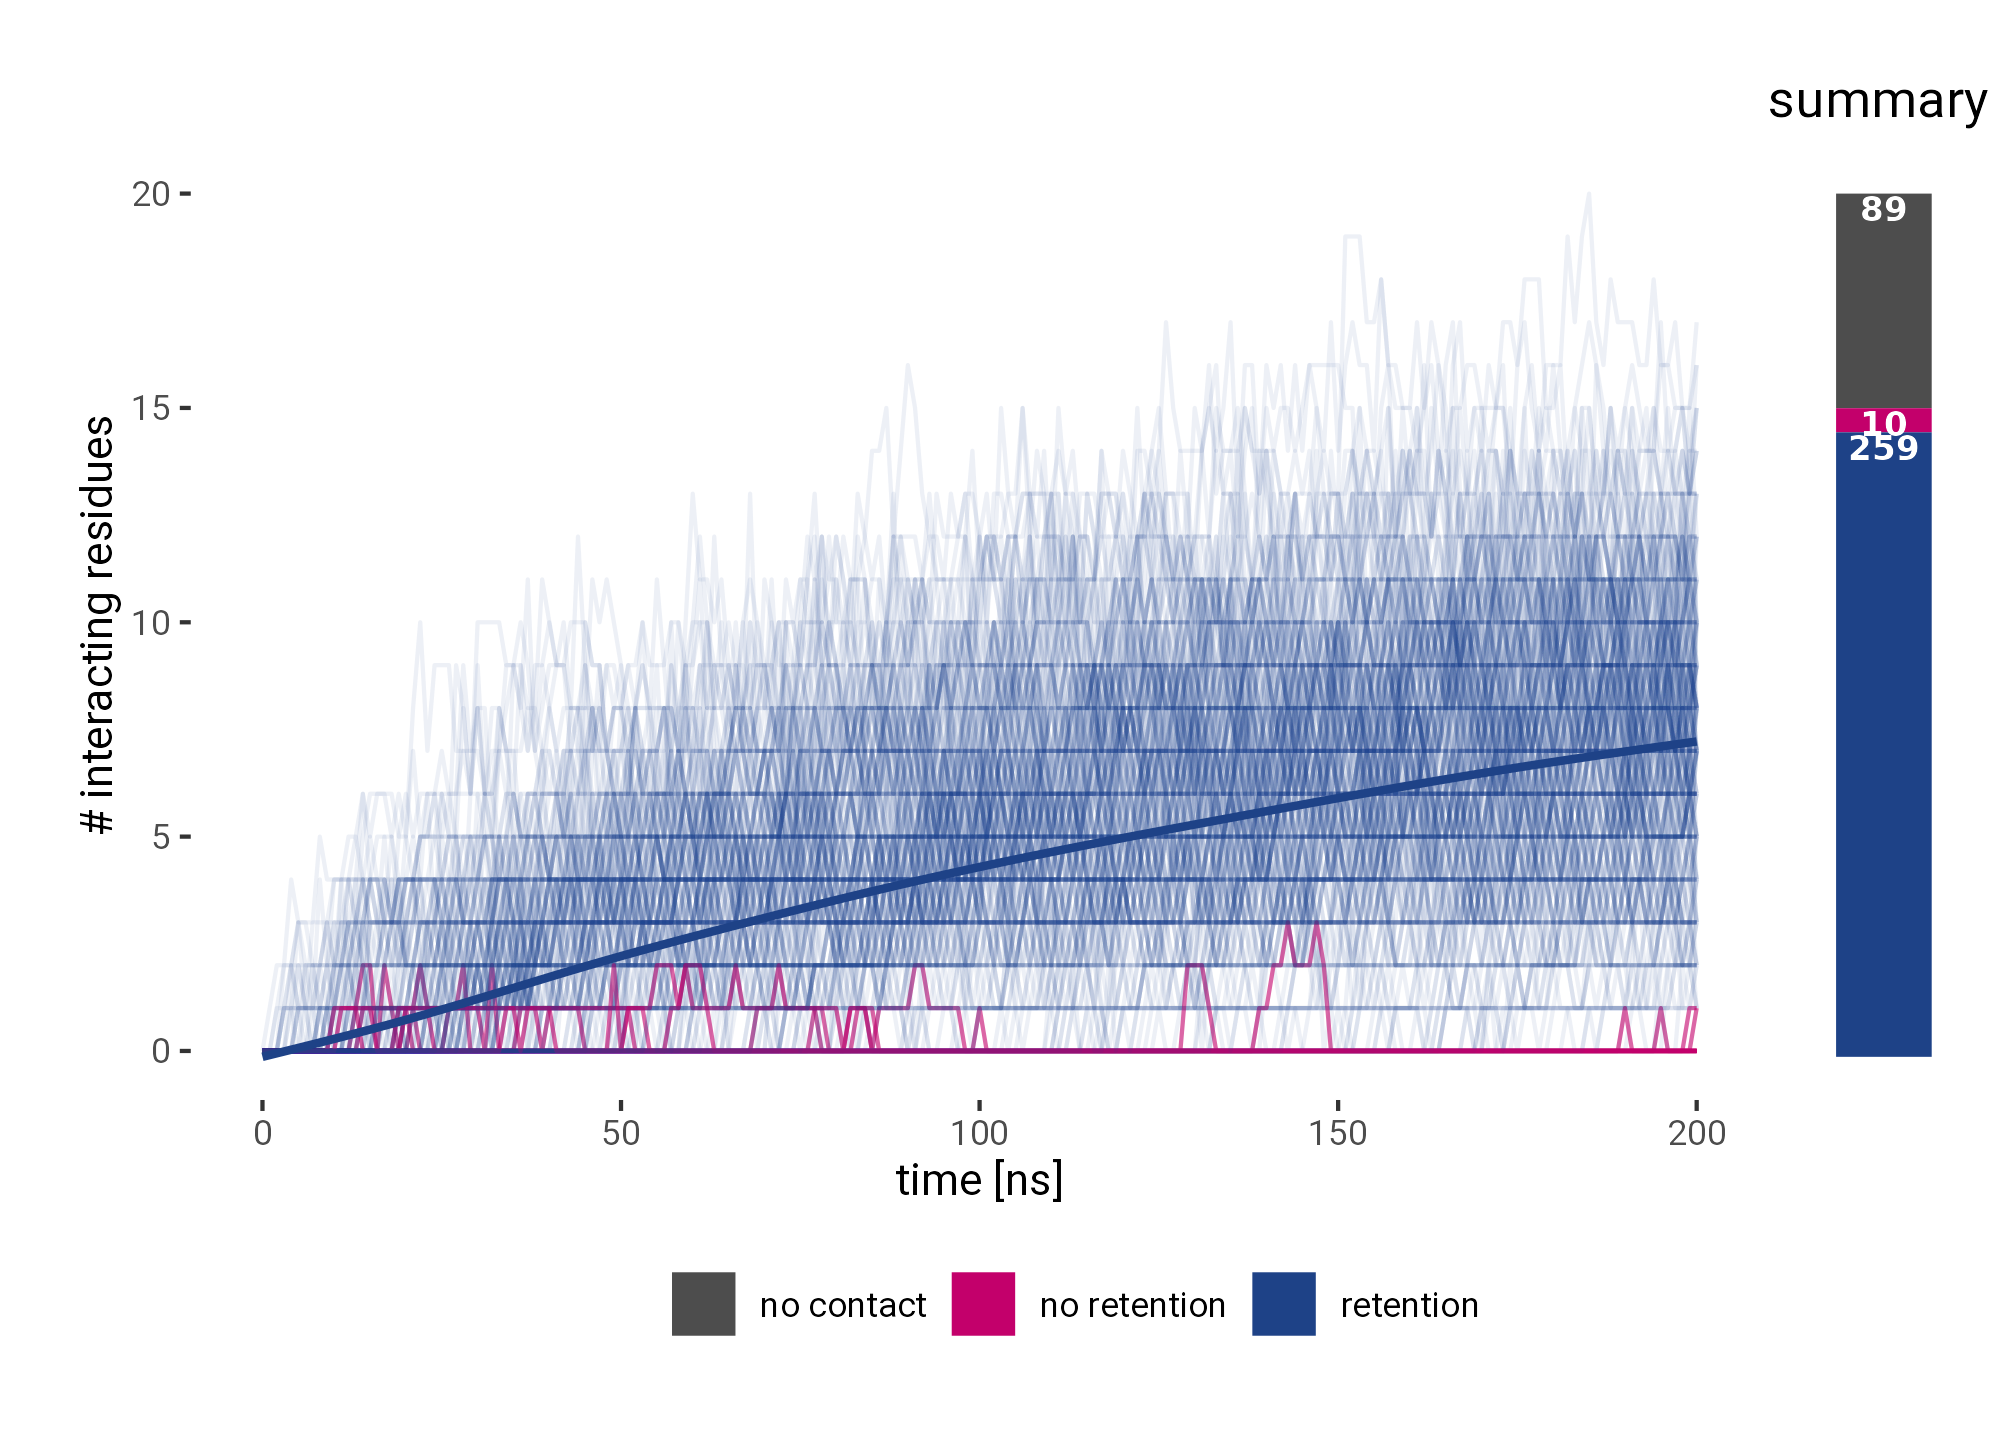
\includegraphics{./results/plots/f0f1-retention-1.png}

}

}

\subcaption{\label{fig-f0f1-retention}~}
\end{minipage}%

\caption{\label{fig-loop-importance-2}Loop--PIP\textsubscript{2}
contacts dynamically accumulate and are mediated by basic residues.
\textbf{a)} Heatmap of the time evolution of the average number of
PIP\textsubscript{2} molecules per residue at the respective time
(y-axis) and angle (x-axis). \textbf{b)} Time evolution (x-axis) of the
number of residues currently interacting with PIP\textsubscript{2}
(y-axis) shows binding and unbinding events and an eventual accumulation
of contacts. Unbinding becomes exceedingly unlikely as the number of
contacts increases.}

\end{figure}

Figure~\ref{fig-f0f1-residues} highlights the residues involved in the
interaction of F0F1 with PIP\textsubscript{2}. The ensemble of final
bound conformations from the simulations can be seen in the
\protect\hyperlink{sec-system}{Supplementary Material}. We observe a
number of prominent lysines and arginines, both positively charged
residues, across the whole F0F1 fragment to compensate for the negative
charge on PIP\textsubscript{2}. The loop region, highlighted with a grey
backdrop in Figure~\ref{fig-f0f1-ri-npip}, is particularly dense in
positively charged residues, albeit the number of PIP\textsubscript{2}
contacts per basic residue is only marginally higher in this region than
elsewhere. Arginines and lysines in regions outside of the disordered
loop complement the binding once initial contacts have been established
with the loop, and further strengthen the interaction. F0 at the
N-terminus (left) is quite flexible as well (see Supplementary Material)
and can thus reasonably contribute towards membrane binding. The
C-terminus of the F1 domain, instead, harbors the interface towards the
F2 domain and the two PIP\textsubscript{2}-interacting residues
identified here will be more occluded \emph{in vivo}. Indeed,
simulations of the full-length FERM domain in the later part of this
work do not show these interactions anymore
(Figure~\ref{fig-ferm-ri-npip}).

\begin{figure}

\begin{minipage}[t]{\linewidth}

{\centering 

\raisebox{-\height}{

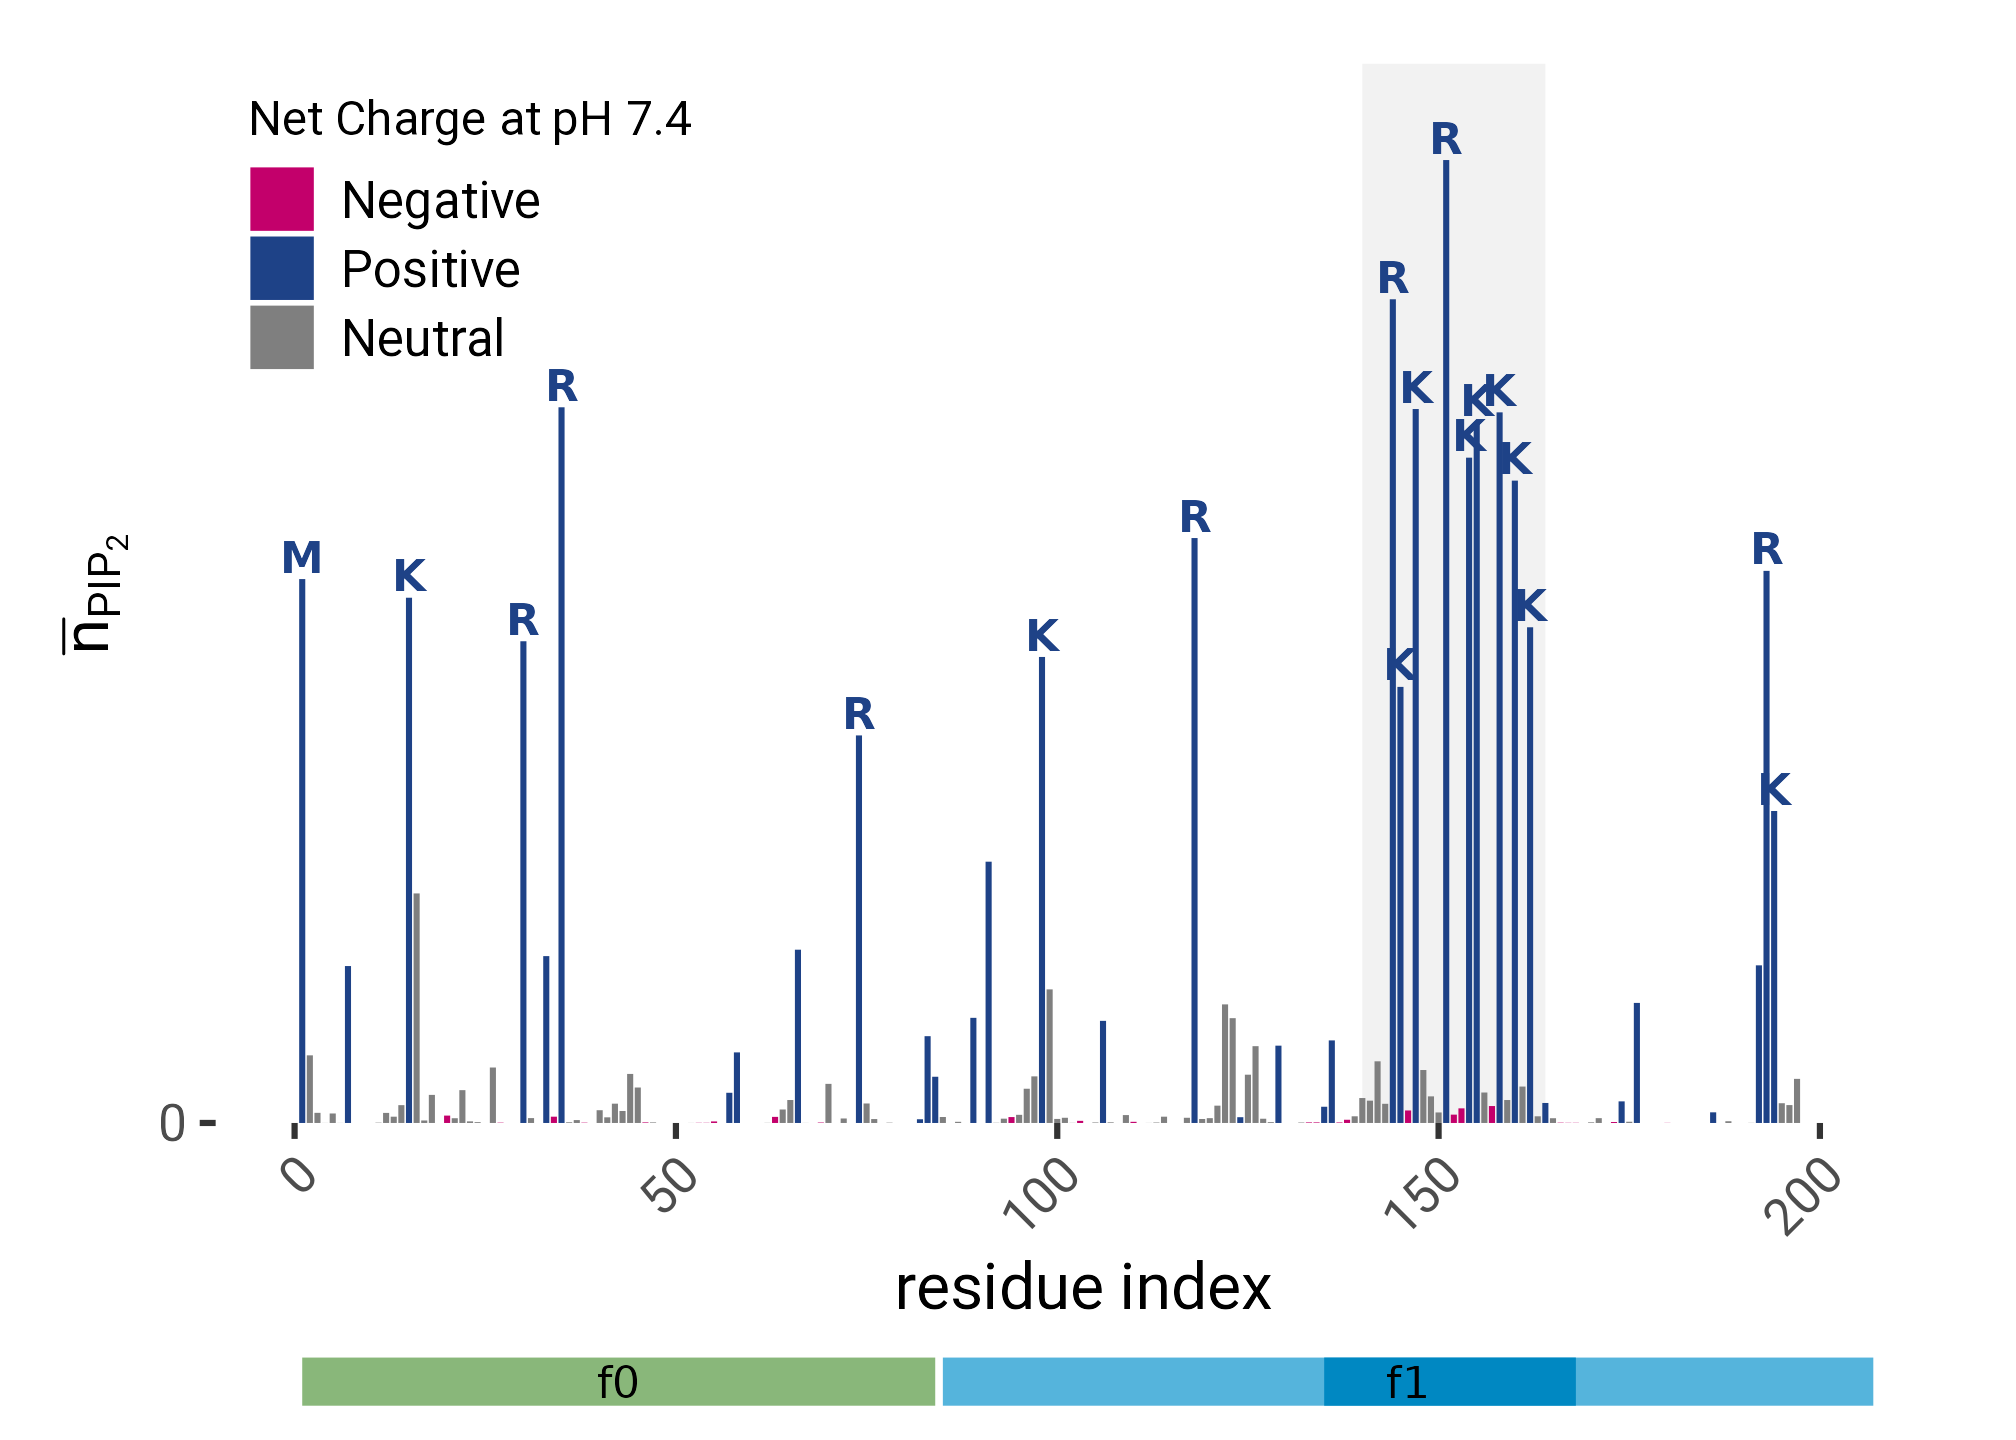
\includegraphics{./results/plots/f0f1-ri-npip-1.png}

}

}

\subcaption{\label{fig-f0f1-ri-npip}~}
\end{minipage}%
\newline
\begin{minipage}[t]{\linewidth}

{\centering 

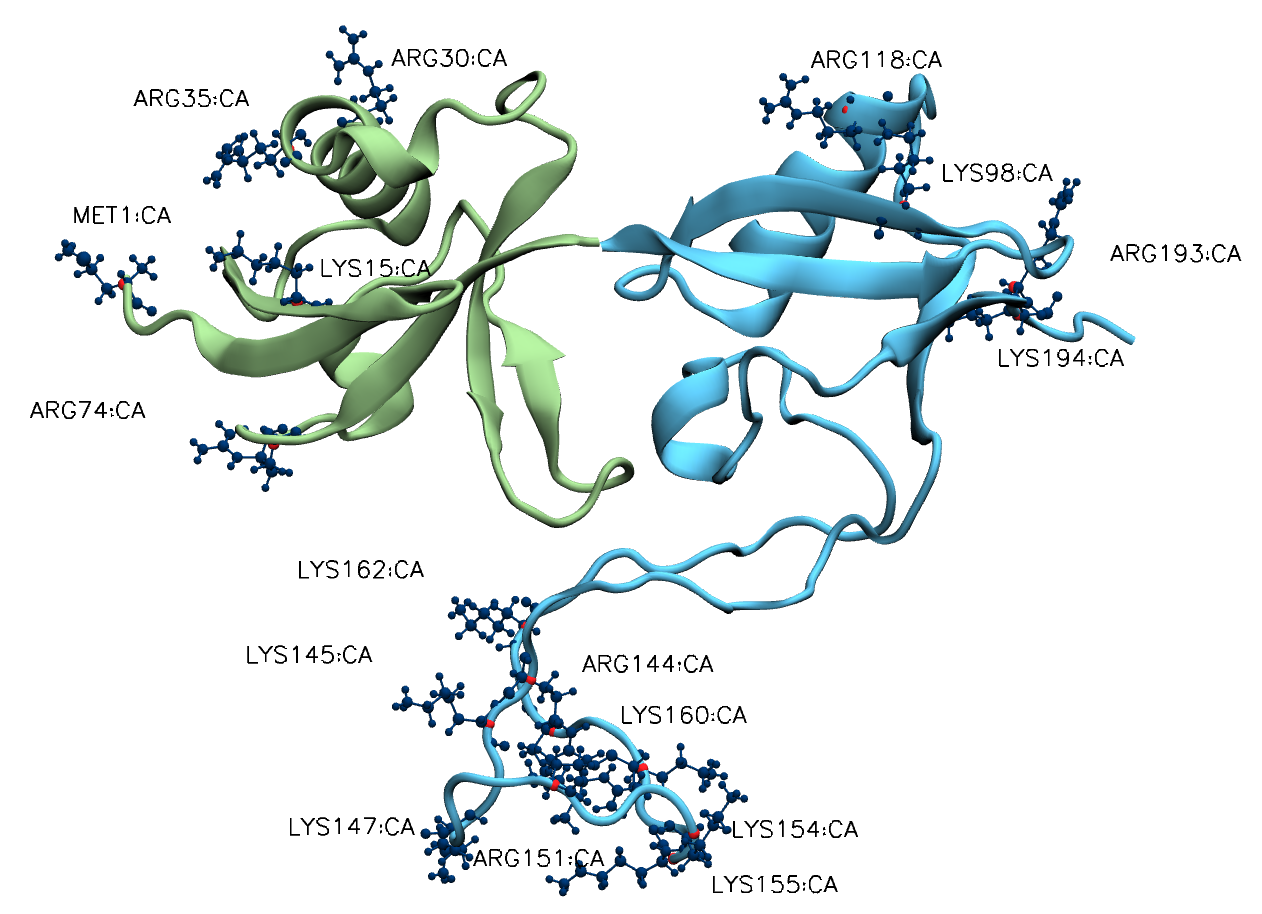
\includegraphics{./assets/vmd/f0f1/residues.png}

}

\subcaption{\label{fig-f1f1-residues}~}
\end{minipage}%

\caption{\label{fig-f0f1-residues}Lysine and arginine residues are
crucial for the PIP\textsubscript{2}-interaction of F0F1. \textbf{a)}
The average number of PIP\textsubscript{2} molecules
(\(\bar n_{PIP_2}\)) interacting (see Supplementary Material for the
interaction distance definition) with the individual residues per frame
across all simulations of the rotational sampling that made contact with
the membrane. Color represents the charge of the amino acid at pH 7.4
(blue = positive/basic, magenta = negative/acidic). A number of very
prominent lysines can be observed, as well as a cluster of residues
belonging to the F1 loop, which is highlighted with a grey backdrop. The
most prominent residues are highlighted in \textbf{b)}. For the print
version it is a snapshot render. The video is also available here:
\url{https://youtu.be/s5yya0XeNTA}).}

\end{figure}

\hypertarget{the-f1-loop-maintains-and-further-facilitates-formation-of-fermpip2-interactions}{%
\subsection{\texorpdfstring{The F1 loop maintains and further
facilitates formation of FERM--PIP\textsubscript{2}
interactions}{The F1 loop maintains and further facilitates formation of FERM--PIP2 interactions}}\label{the-f1-loop-maintains-and-further-facilitates-formation-of-fermpip2-interactions}}

To examine the strength of the PIP\textsubscript{2} interactions and the
role of the F1 loop in maintaining it, we pulled F0F1 vertically off the
membrane in additional force-probe MD simulations
(Figure~\ref{fig-f0f1-vert-pull}). An exemplary render of one of the
simulations can be seen in Figure~\ref{fig-f0f1-pull-run-1}. Pulling
F0F1 off the membrane requires peak forces of 100--120~pN, during which
the interacting residues only very gradually loose contact
(Figure~\ref{fig-f0f1-vert-pull}), as the high flexibility of F1-loop
allows the residues to remain in contact even as the distance increases
up to a delta of 7~nm. Replicate 4 stands out as the highest curve
(dashed lines), as in this run the interactions were so strong that a
total of 3 molecules of PIP\textsubscript{2} were pulled out of the
membrane (1 by F0 and 2 by the F1 loop). A snapshot of this can be seen
in the Supplementary Material in Figure 8b. This highlights the strong
anchoring capabilities of the F1 loop.

As seen in Figure~\ref{fig-f0f1-vert-pull-contacts}, during pulling
residues not belonging to the F1 loop loose contact first, while the
loop stays attached. The F1 loop works in conjunction with the F0
subdomain. Their high flexibility allows them to remain in contact with
the membrane over large distances, which would allow for a spring-like
re-establishing of more contacts should the force be alleviated. In two
cases the last interacting residue was part of the F1 loop, while in
three cases the N-terminus of the F0 domain stayed attached for longest.

\begin{figure}

\begin{minipage}[t]{\linewidth}

{\centering 

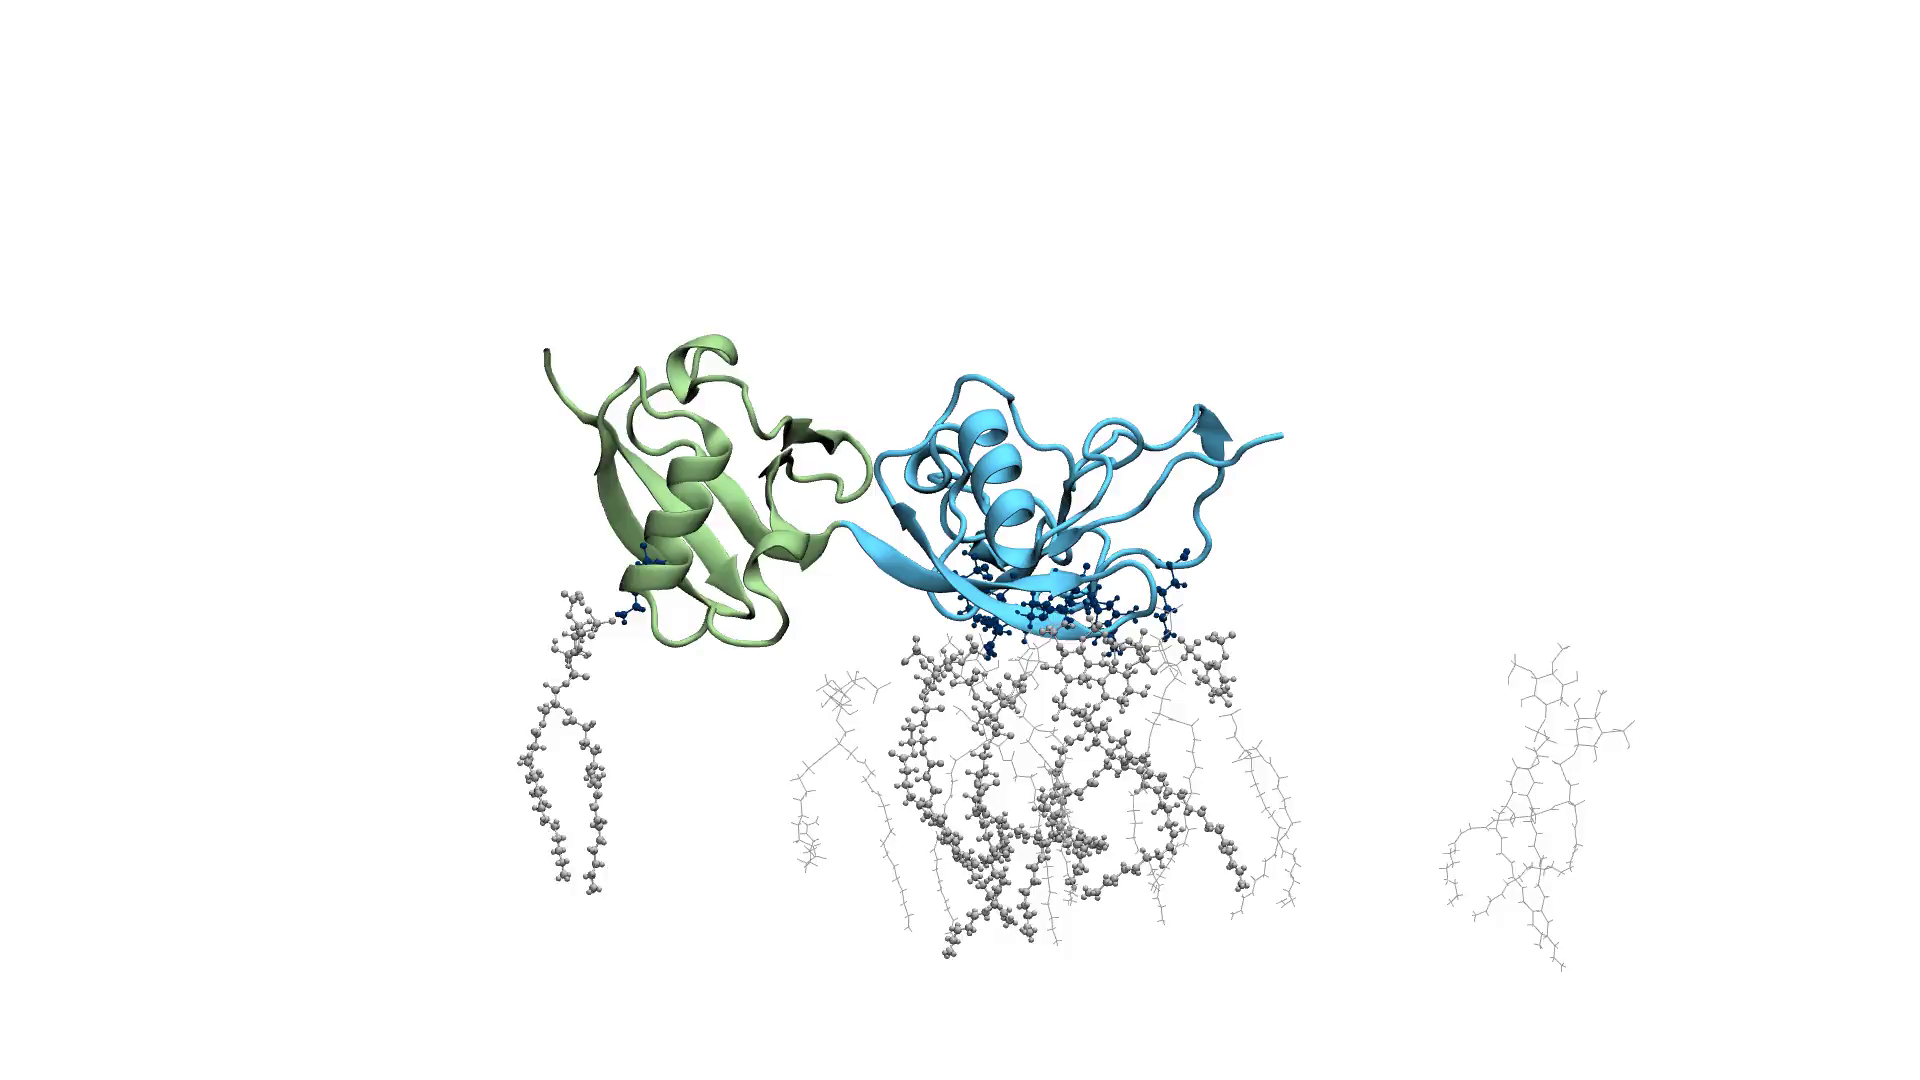
\includegraphics[width=0.35\textwidth,height=\textheight]{./assets/vmd/f0f1-pulling/f0f1-pull-start.png}
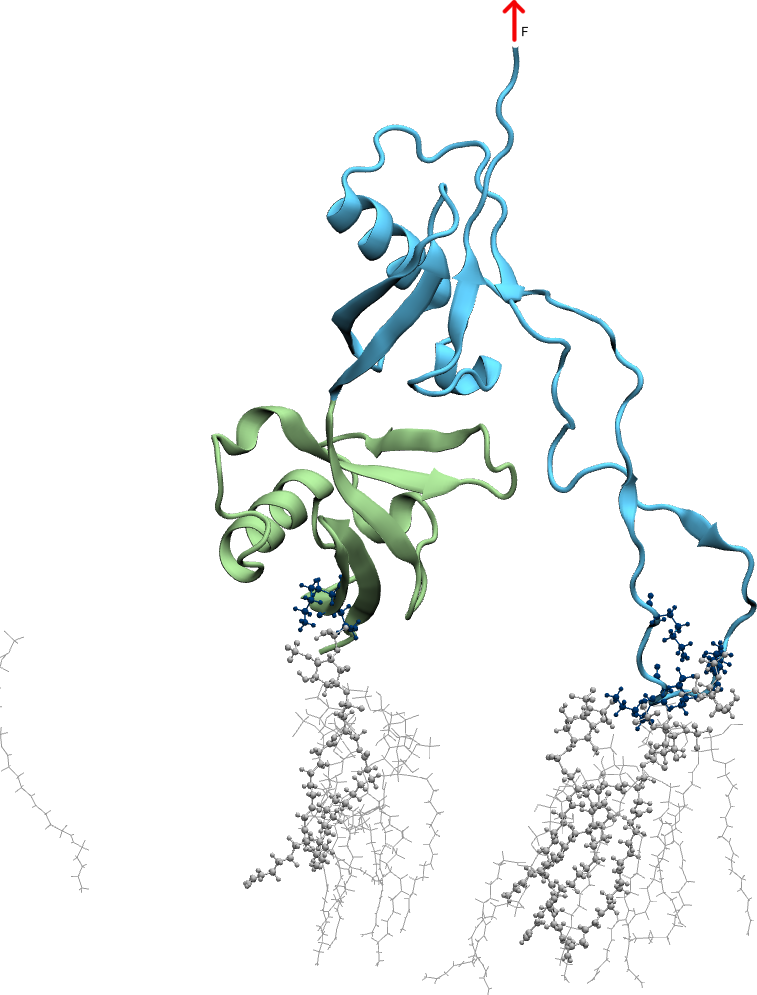
\includegraphics[width=0.2\textwidth,height=\textheight]{./assets/vmd/f0f1-pulling/f0f1-pull-middle.png}
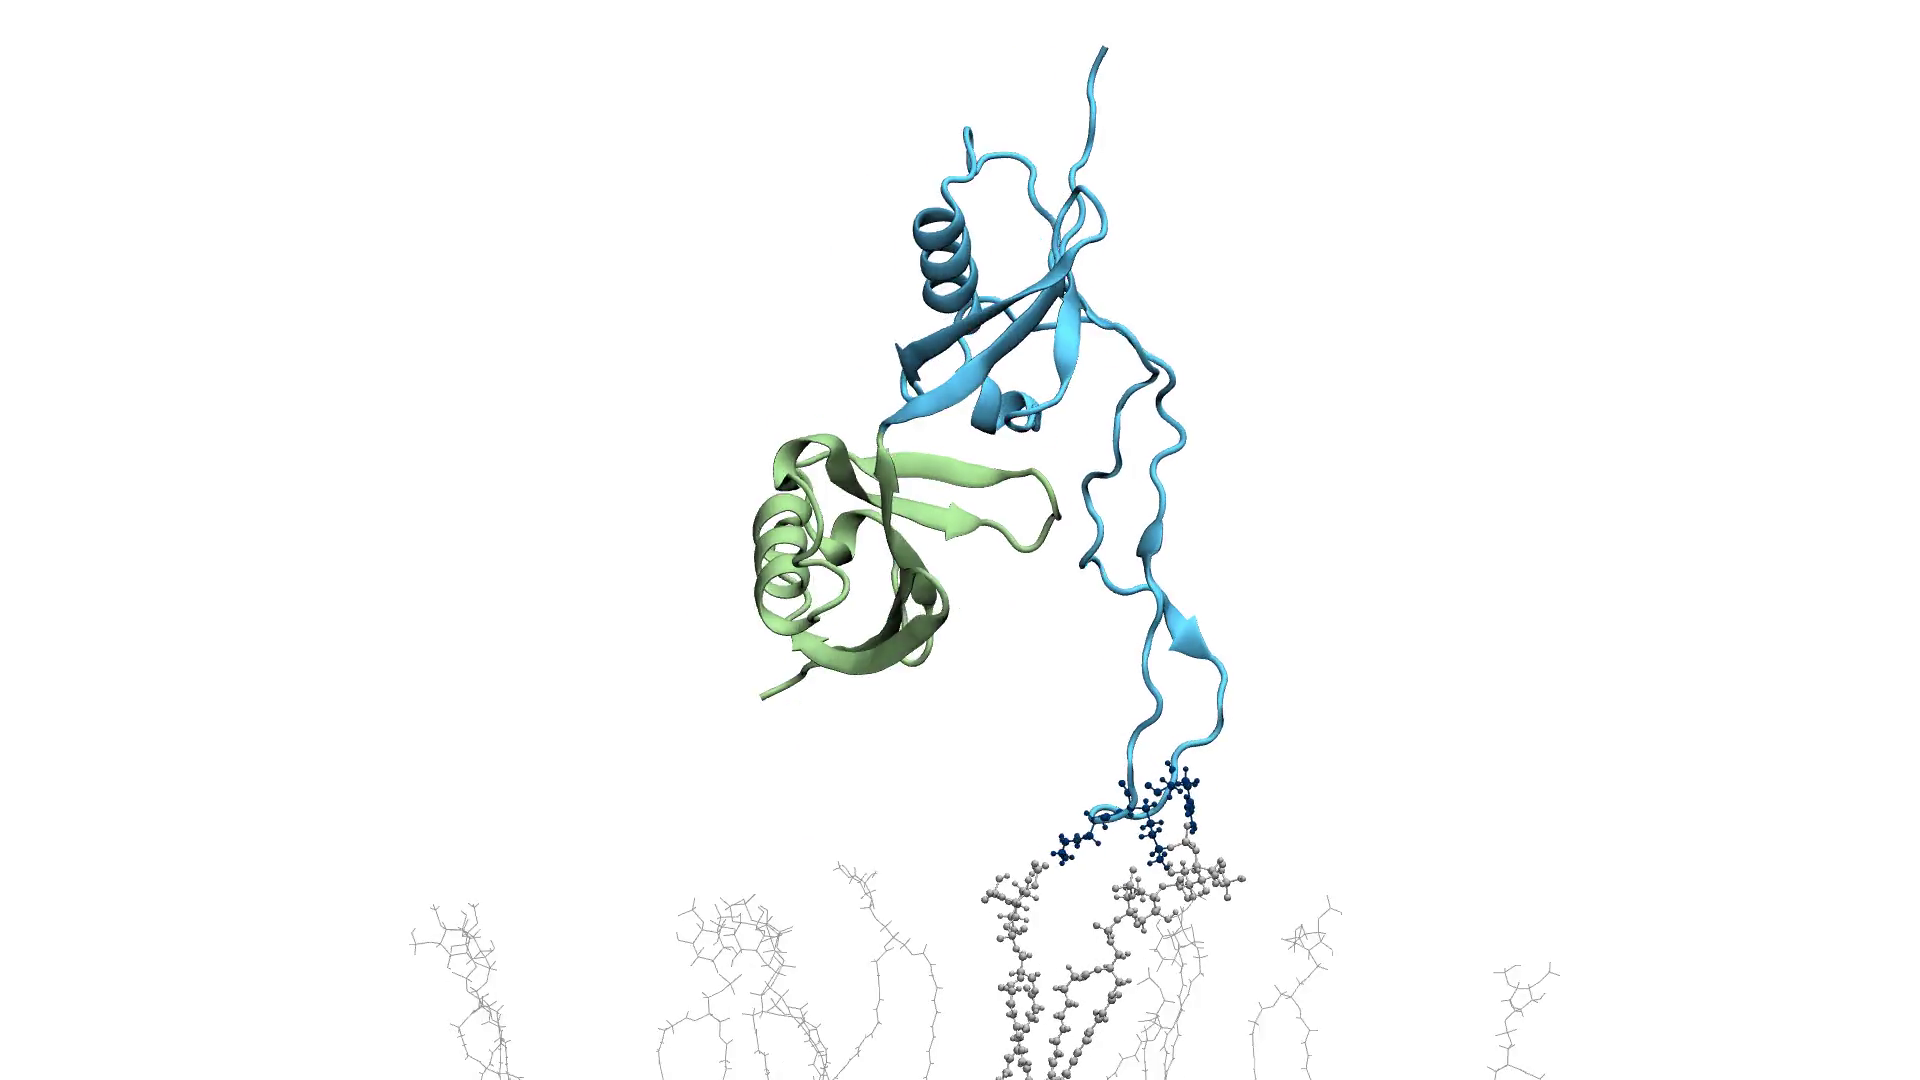
\includegraphics[width=0.35\textwidth,height=\textheight]{./assets/vmd/f0f1-pulling/f0f1-pull-end.png}

}

\subcaption{\label{fig-f0f1-pull-run-1}~}
\end{minipage}%
\newline
\begin{minipage}[t]{0.50\linewidth}

{\centering 

\raisebox{-\height}{

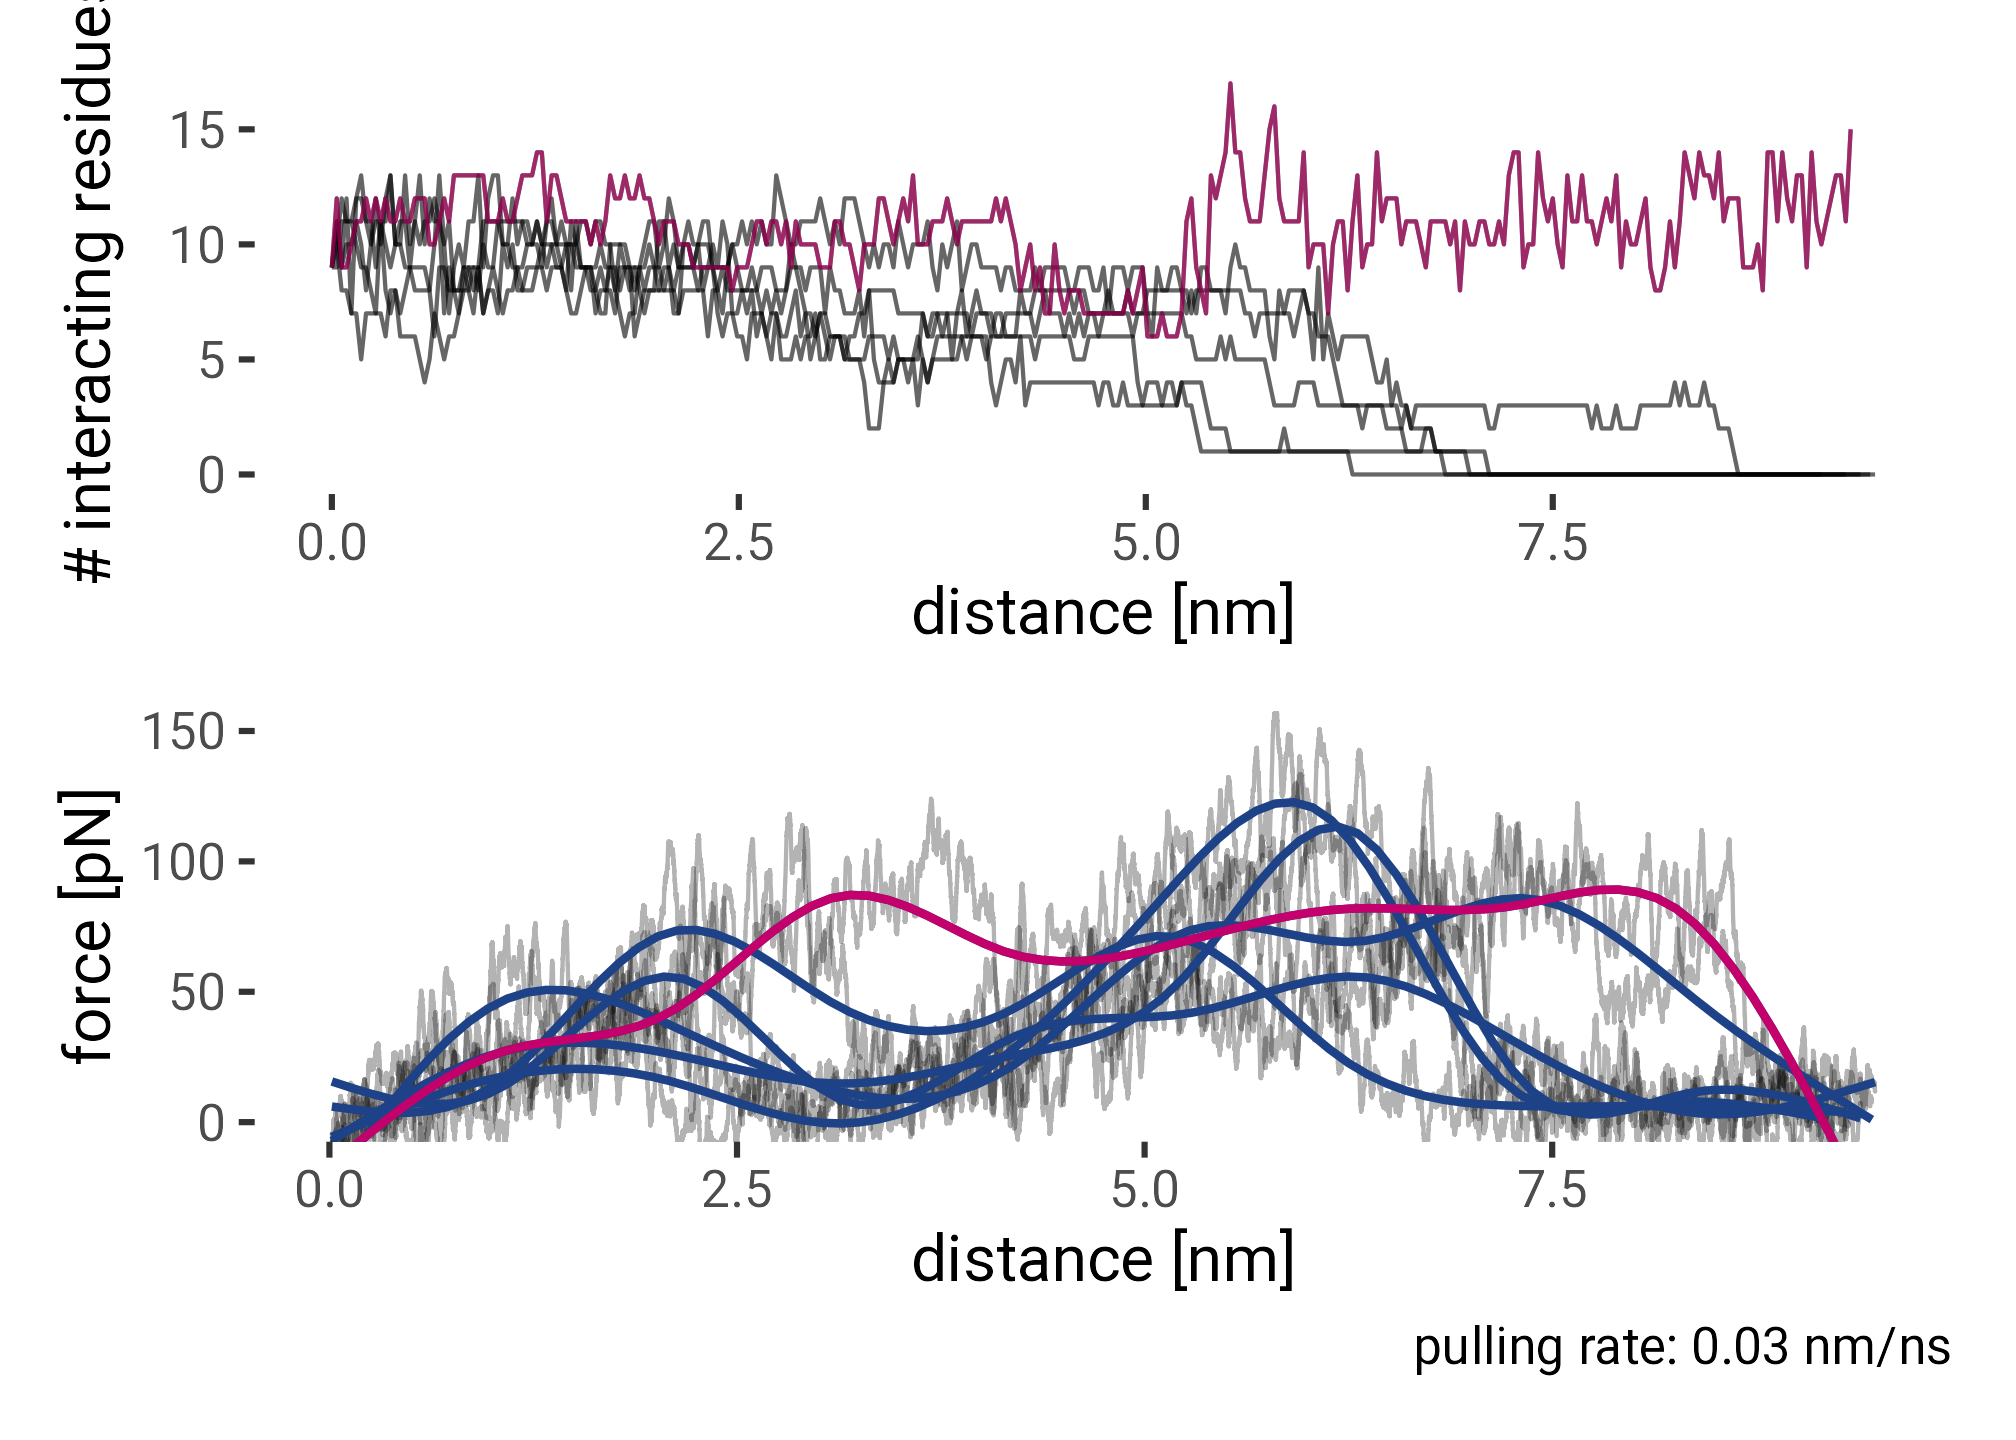
\includegraphics{./results/plots/f0f1-vert-pull-1.png}

}

}

\subcaption{\label{fig-f0f1-vert-pull-force}~}
\end{minipage}%
%
\begin{minipage}[t]{0.50\linewidth}

{\centering 

\raisebox{-\height}{

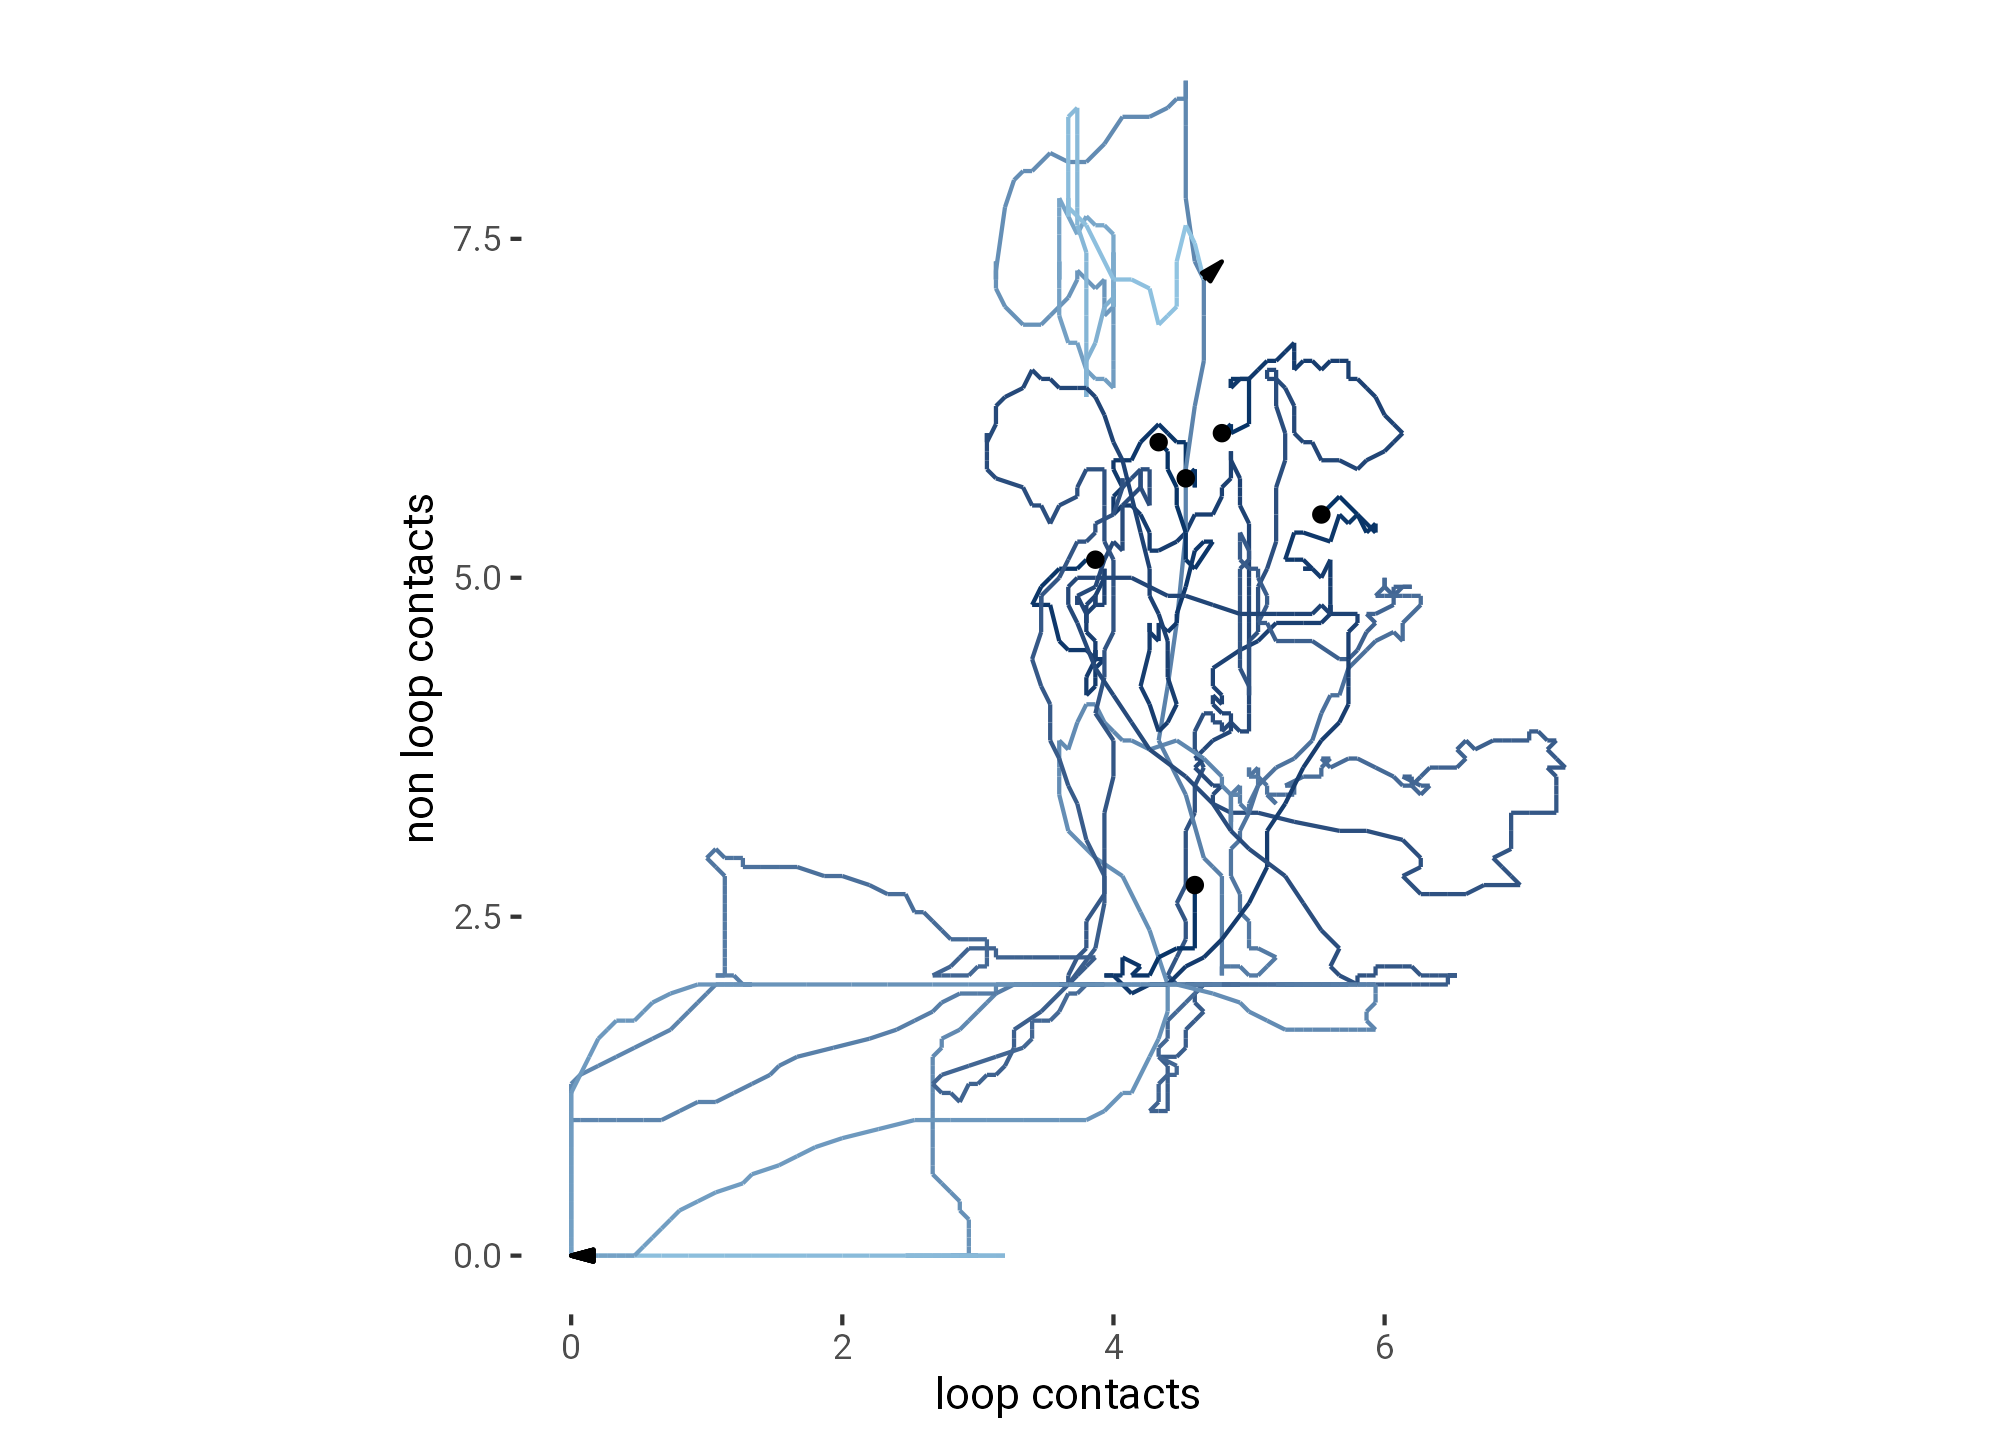
\includegraphics{./results/plots/f0f1-vert-pull-contacts-time-1.png}

}

}

\subcaption{\label{fig-f0f1-vert-pull-contacts}~}
\end{minipage}%

\caption{\label{fig-f0f1-vert-pull}Vertical pulling of F0F1 highlights
the F1 loop's flexibility and ability to maintain contacts with the
membrane over large distances. \textbf{a)} Representative render of one
of 6 force-probe MD simulations pulling F0F1 off the membrane. For the
print version we show a series of three snapshots, the video is
available here: \url{https://youtu.be/-eZ2orx7QRE}. It starts from a
snapshot of F0F1 in its bound conformation taken from the rotational
sampling and gets pulled upwards from its C-terminus. \textbf{b)} Number
of interacting residues (top panel) and the force (bottom panel) as a
function of distance (x-axis) as F0F1 gets pulled off the membrane at a
constant rate of 0.03~nm/ns. \textbf{c)} Time evolution of the number of
contacts for residues belonging to the F1 loop (x-axis) and other
residues (y-axis). Traces are colored by replicate. Black dots mark the
starting positions. The non-loop contacts are mostly supplied by the
residues of the F0 N-terminus also shown in
Figure~\ref{fig-f0f1-ri-npip}.}

\end{figure}

Having established the prominent role of the F1-loop in positioning F0F1
at the membrane and establishing PIP\textsubscript{2} contacts, we next
examined this role in the larger context of the full FERM domain. 6
independent simulations were initiated with the full-length FERM domain
oriented in such that the tip of the F1-loop was in contact with at
least one molecule of PIP\textsubscript{2} with varying local
environments (see \protect\hyperlink{sec-system}{Simulation Systems and
Structures} for one example). Individual interaction heatmaps for each
run can be found in the Supplementary Material. These simulations
highlight the prominent role of the F1-loop in membrane interactions,
now in the context of the full-length FERM domain
(Figure~\ref{fig-ferm-ri-npip}, compare to
Figure~\ref{fig-f0f1-ri-npip}). They also reproduce the canonical
PIP\textsubscript{2} contacts in F2 and F3 known from previous studies,
validating our MD simulations. The highlighted residues include K272 of
F2 and K316, K324, E342, and K343 of F3, which have been shown to be
crucial for the membrane interaction of talin and subsequent integrin
activation by Chinthalapudi et al.
(\protect\hyperlink{ref-chinthalapudiInteractionTalinCell2018a}{20}).
Importantly, the loop shows a very dense cluster of PIP\textsubscript{2}
interactions, with interaction scores (\(\bar n_{PIP_2}\)) very similar
to these previously known PIP\textsubscript{2}-interacting residues. The
interacting conformations can be seen in context in the
\protect\hyperlink{sec-system}{Supplementary Material}. The F1 loop thus
complements these known binding sites with an additional specific
binding site, again comprising primarily lysines.

\begin{figure}

\begin{minipage}[t]{\linewidth}

{\centering 

\raisebox{-\height}{

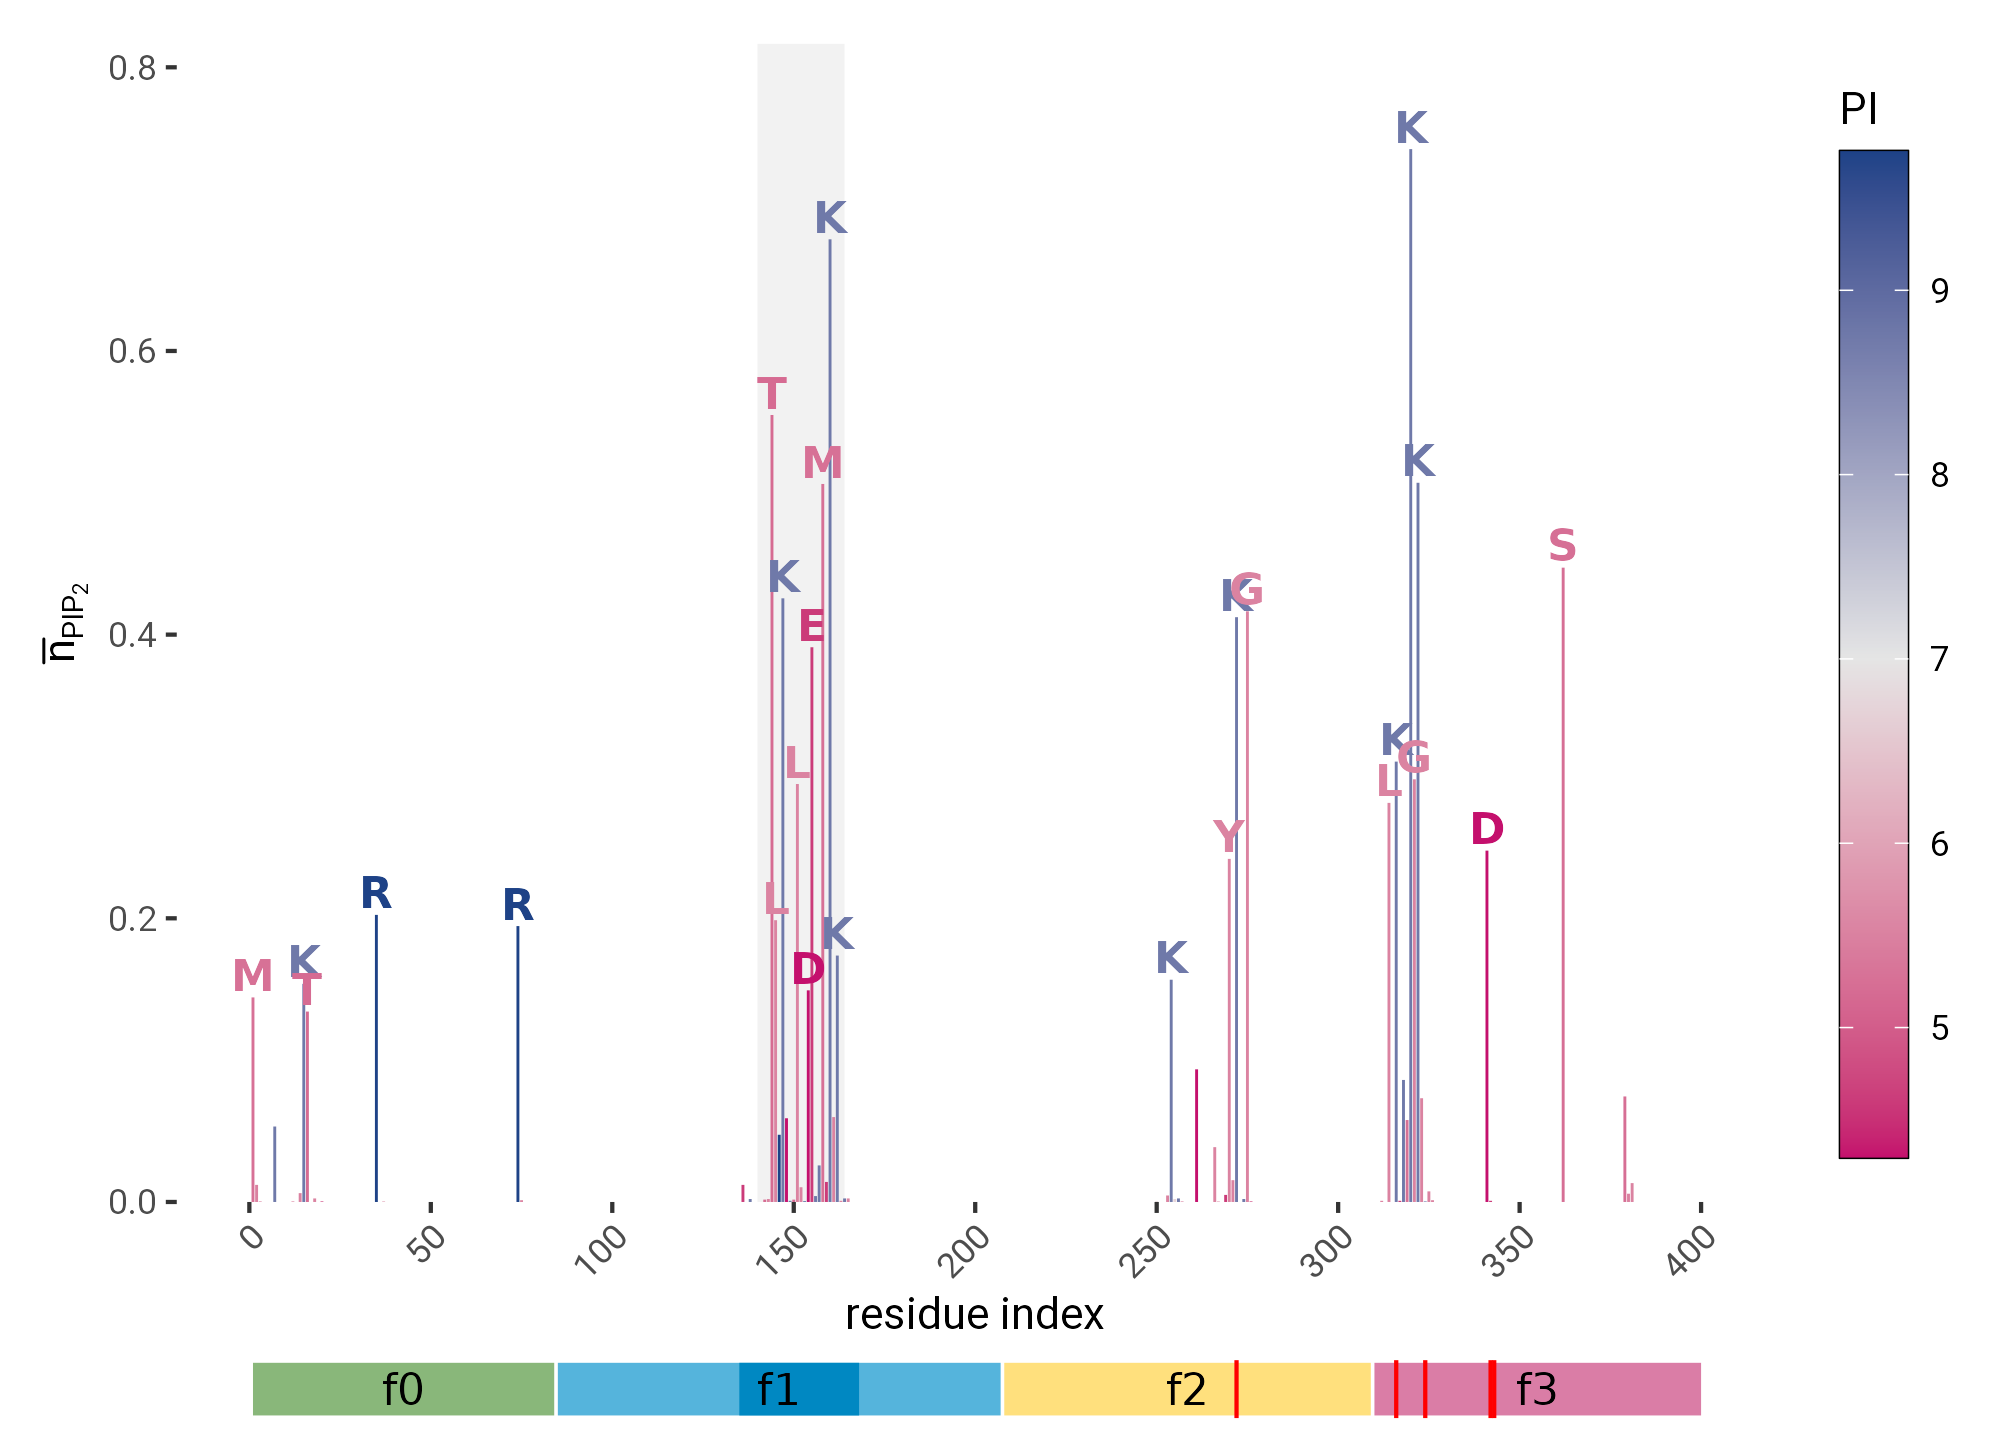
\includegraphics{./results/plots/ferm-ri-npip-1.png}

}

}

\subcaption{\label{fig-ferm-ri-npip}~}
\end{minipage}%
\newline
\begin{minipage}[t]{\linewidth}

{\centering 

\raisebox{-\height}{

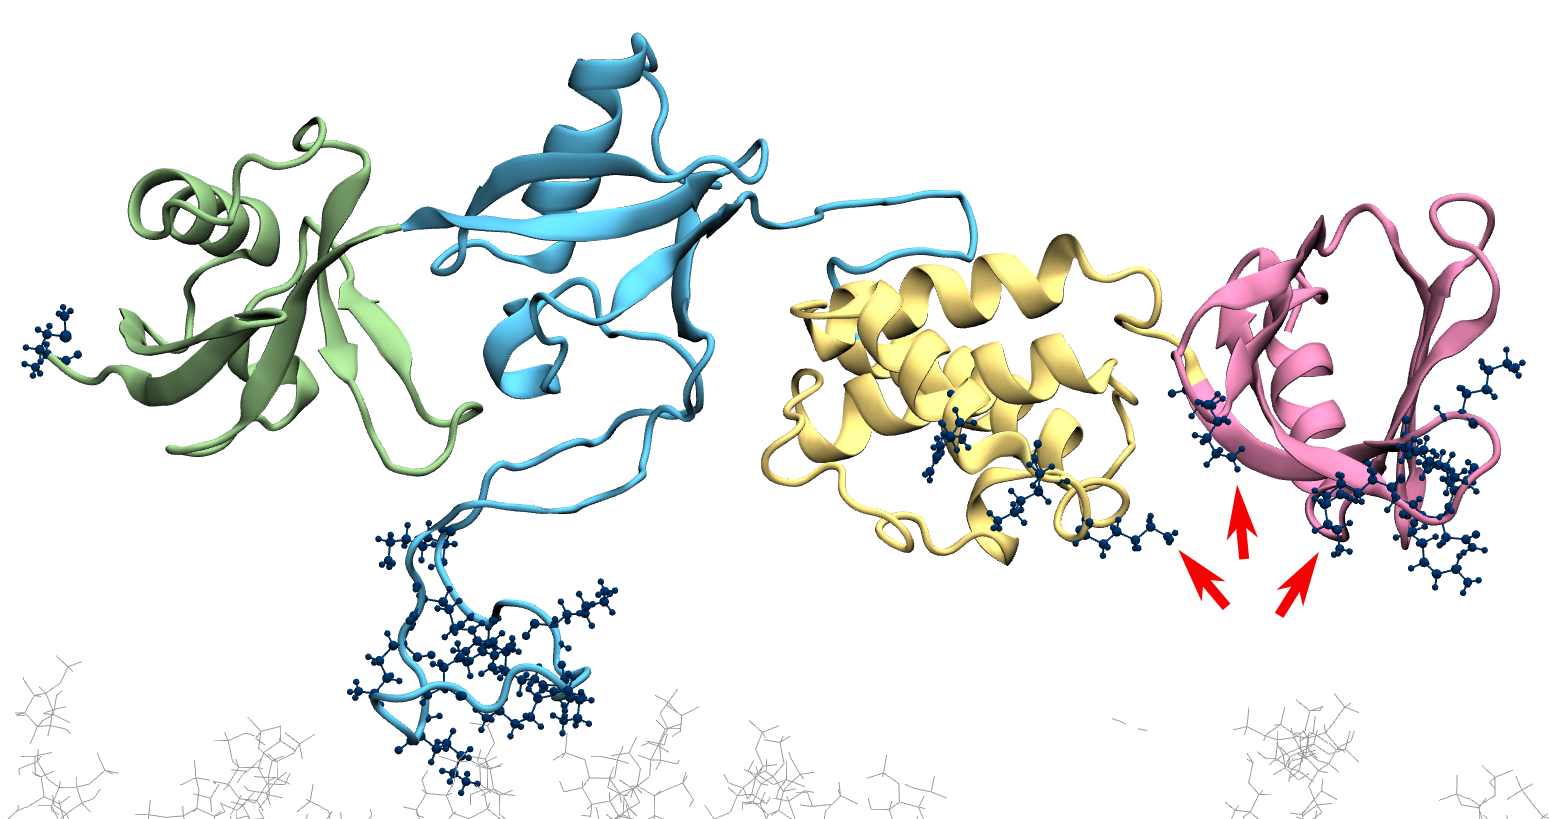
\includegraphics{./assets/vmd/ferm/ferm-residues-transparent-arrows.png}

}

}

\subcaption{\label{fig-ferm-memb-system}~}
\end{minipage}%

\caption{\label{fig-ferm-further}Simulation of the full-length FERM
domain over a 10\% PIP\textsubscript{2}-membrane. \textbf{a)} The
average number of PIP\textsubscript{2} molecules interacting with the
individual residues across 6 simulations. Color represents the charge of
the amino acid at pH 7.4 (blue = positive/basic, magenta =
negative/acidic). The known PIP\textsubscript{2} interaction sites K272
of F2 and K316, K324, E342, and K343 of F3
(\protect\hyperlink{ref-chinthalapudiInteractionTalinCell2018a}{20}) are
highlighted with red lines on the x-axis colorbar and can also be seen
in the cartoon representation in \textbf{b)} where the interacting
residues with a score greater than 0.2 are displayed as dark blue stick
models.}

\end{figure}

\hypertarget{discussion-and-outlook}{%
\section{Discussion and Outlook}\label{discussion-and-outlook}}

Using atomistic MD simulations, we provide mechanistic insight into the
membrane recognition dynamics of talin. Our simulations propose a new
mode of interaction that helps to explain how talin can bind the
membrane even when its main PIP\textsubscript{2} (and integrin) binding
sites in F2 and F3
(\protect\hyperlink{ref-chinthalapudiInteractionTalinCell2018a}{20})
(see figure Figure~\ref{fig-ferm-memb-system} ) are blocked by
autoinhibition
(\protect\hyperlink{ref-deddenArchitectureTalin1Reveals2019a}{23}).
Specifically, we find the unique unstructured, 33-residue-long insertion
into the F1 domain, the F1 loop, to provide a strong interaction anchor
to PIP\textsubscript{2}-containing membranes.

Overall, the FERM--membrane interaction mode is not characterized by
singular binding sites interacting with one molecule of
PIP\textsubscript{2} each, as would be the conclusion from
crystallographic data alone. Rather the cumulative diffuse interaction
of multiple PIP\textsubscript{2} with multiple residues is what keeps
the protein anchored to the membrane. This is particularly evident in
the interaction with the flexible F1 loop, but also in the F0 domain.
While crystal structures of proteins in complex with
PIP\textsubscript{2} typically show a one-to-one ratio of lipid per
binding site
(\protect\hyperlink{ref-chinthalapudiInteractionTalinCell2018a}{20},
\protect\hyperlink{ref-chinthalapudiLipidBindingPromotes2018}{48},
\protect\hyperlink{ref-jianMolecularBasisCooperative2015}{49}), possibly
due to the nature of the experimental method, our simulations suggest
multiple PIP\textsubscript{2} molecules binding simultaneously. Similar
results have been observed for Pleckstrin Homology (PH) domain proteins
by Naughton et al.
(\protect\hyperlink{ref-naughtonModesInteractionPleckstrin2018}{50}).
According to their study, this simultaneous binding of multiple
PIP\textsubscript{2} molecules contributes to the high affinity of the
membrane interaction.

Our MD simulations suggest that the F1 loop can find favorable
interactions with PIP\textsubscript{2} across large distances and in a
large search volume. We find this to be the disordered loop's high
flexiblity. The F1 loop can maintain the membrane contacts when talin is
pulled off of the membrane over distances as large as 7~nm. A similar
mechanism has also been shown by Shoemaker et al.
(\protect\hyperlink{ref-shoemakerSpeedingMolecularRecognition2000}{51})
and was fittingly coined ``fly-casting''. In the aforementioned
publication they focus on the interaction of unfolded regions with DNA.
Our simulations now provide an example for the concept applied to
protein-lipid interactions. It is well worth noting that, although we
mention the greater search space of the F1 loop as its advantage in
recognizing PIP\textsubscript{2}, it has also been argued that the
kinetic advantage of the fly-casting mechanism comes mainly from the
reduction in free energy as the disordered region folds around the
interaction target
(\protect\hyperlink{ref-huangKineticAdvantageIntrinsically2009}{52}).
This can also be argued here, as the loop can flexibly adapt its
conformation to the membrane and the dynamic distribution of
PIP\textsubscript{2} lipids therein. As such it can bind in a
multivalent fashion, with several basic residues binding to several
PIP\textsubscript{2} lipids.

Fast binding kinetics are crucial for talin's function at focal adhesion
sites. As the PIP\textsubscript{2} concentrations increases at the
active focal adhesion site, talin's FERM F1 loop can perform rapid
recognition. The flexibility of the loop also allows it to anchor the
protein at the membrane even when being stretched under force (up to a
delta of 7~nm, as seen in Figure~\ref{fig-f0f1-vert-pull}). This is akin
to the elastic response seen in focal adhesion kinase (FAK) under force,
in which a 49-residue-long linker allows for buffering of the force
(\protect\hyperlink{ref-bauerStructuralMechanisticInsights2019}{53}).
Here, talin's F1 loop can extend and thereby maintain the interactions,
which could help rapid rebinding when the force is relieved.

In our force probe simulations, we pulled F0F1 orthogonally off the
membrane. This allowed us to assess the full extension and force
resistance of the loop. \emph{In vivo}, however, talin's FERM domain is
subjected to forces acting at a 30° angle. This might imply an
additional function for the FERM domain. As it is dragged along the
membrane, the diffuse interactions of the F1 loop and main interaction
sites in F2-F3 with PIP\textsubscript{2} would increase lateral friction
along the membrane as the PIP\textsubscript{2} concentration increases.
This could further localize talin at active focal adhesion sites even in
the presence of forces acting parallel to the membrane.

We conclusively show that the F1 loop is able to interact with the
membrane even from most unfavorable orientations. The role of the F1
loop in this is kinetic in nature. Previous studies have shown F0F1 to
not significantly influence the binding equilibrium of a FERM domain to
immobilized PIP\textsubscript{2}-containing membranes compared to
constructs containing only F2F3
(\protect\hyperlink{ref-mooreAffinityTalin1V3integrin2012a}{54}). Also,
when the main binding site in F2F3 was mutated, another study using
lipid co-sedimentation found that the F1-loop alone does not suffice to
restore lipid binding
(\protect\hyperlink{ref-chinthalapudiInteractionTalinCell2018a}{20}).
Our study suggests that while the thermodynamics of binding might remain
unchanged, the equilibrium should be reached faster due to the presence
of the loop. We propose that talin mutants lacking the loop, or
specifically the basic residues in said loop, will show reduced or at
least slowed-down focal adhesion maturation, increased lateral diffusion
of talin under force, and faster focal adhesion disassembly. We note
that given the high disorder of the F1 loop, we speculate that this
interaction is rather unspecific compared to the
PIP\textsubscript{2}-specific F2F3 site, and interactions with
PIP\textsubscript{3} are also likely to form. To what extent our
conclusions are also applicable to talin-2 remains to be shown. Given
the high sequence similarity and conservation of the F1 loop
(\protect\hyperlink{ref-goultStructureDoubleUbiquitinlike2010}{13}), we
speculate that it plays a similar role as early PIP\textsubscript{2}
anchor in the talin-2 isoform as well.

Recognition is only the first step. The mechanistic details of how
talin's autoinhibition is resolved remain to be shown by larger
simulations including the inhibiting rod segment. These larger-scale
simulations might then be able to provide evidence for the push--pull
mechanism proposed by Song et al.
(\protect\hyperlink{ref-songNovelMembranedependentSwitch2012a}{12}) or
might reveal how the early F1-loop mediated membrane interactions
identified in this study might effect the subsequent steps for talin
activation.

As the F1-loop has been shown to contribute to integrin activation
(\protect\hyperlink{ref-goultStructureDoubleUbiquitinlike2010}{13}), it
will also be insightful to simulate a system including the integrin
tail. This is a promising approch, since other computational studies
have also found PIP\textsubscript{2} to be crucial, not just for the
membrane interaction, but also the formation of the protein--protein
complex. The cloverleaf-like FERM domain of moesin, for example,
interacts with the cytoplasmic domain of L-selectin mediated by
PIP\textsubscript{2}
(\protect\hyperlink{ref-sunMolecularDynamicsAssociation2018}{55}) and
PIP\textsubscript{2} enables the formation of the CD44-FERM complex for
radixin
(\protect\hyperlink{ref-sunMolecularMechanismBidirectional2020}{56}).

In conclusion, we propose positively charged, intrinsically disordered
regions in talin's FERM domain and potentially other
PIP\textsubscript{2}-binding domains to promote fast recognition and to
help maintain the membrane interaction under force.

\hypertarget{author-contributions}{%
\section{Author Contributions}\label{author-contributions}}

Conceived and designed the experiments:~JB FF FG. Performed the
experiments:~JB FF. Analyzed the data:~JB FF. Contributed
reagents/materials/analysis tools:~FF. Wrote the paper:~JB FF.

\hypertarget{declaration-of-interests}{%
\section{Declaration of Interests}\label{declaration-of-interests}}

The authors declare no competing interests.

\hypertarget{acknowledgments}{%
\section{Acknowledgments}\label{acknowledgments}}

This work was supported by the Klaus Tschira Foundation and the European
Research Council (ERC) under the European Union's Horizon 2020 research
and innovation programme (grant agreement No.~101002812).

\hypertarget{references}{%
\section{References}\label{references}}

\hypertarget{refs}{}
\begin{CSLReferences}{0}{0}
\leavevmode\vadjust pre{\hypertarget{ref-vogelLocalForceGeometry2006}{}}%
\CSLLeftMargin{1. }%
\CSLRightInline{Vogel, V., and M. Sheetz. 2006.
\href{https://doi.org/10.1038/nrm1890}{Local force and geometry sensing
regulate cell functions}. \emph{Nature Reviews Molecular Cell Biology}.
7:265--275.}

\leavevmode\vadjust pre{\hypertarget{ref-oakesStressingLimitsFocal2014}{}}%
\CSLLeftMargin{2. }%
\CSLRightInline{Oakes, P.W., and M.L. Gardel. 2014.
\href{https://doi.org/10.1016/j.ceb.2014.06.003}{Stressing the limits of
focal adhesion mechanosensitivity}. \emph{Current Opinion in Cell
Biology}. 30:68--73.}

\leavevmode\vadjust pre{\hypertarget{ref-schillerMechanosensitivityCompositionalDynamics2013}{}}%
\CSLLeftMargin{3. }%
\CSLRightInline{Schiller, H.B., and R. Fässler. 2013.
\href{https://doi.org/10.1038/embor.2013.49}{Mechanosensitivity and
compositional dynamics of cell\textendash matrix adhesions}. \emph{EMBO
reports}. 14:509--519.}

\leavevmode\vadjust pre{\hypertarget{ref-miroshnikovaAdhesionForcesCortical2018}{}}%
\CSLLeftMargin{4. }%
\CSLRightInline{Miroshnikova, Y.A., H.Q. Le, D. Schneider, T. Thalheim,
M. Rübsam, N. Bremicker, J. Polleux, N. Kamprad, M. Tarantola, I. Wang,
M. Balland, C.M. Niessen, J. Galle, and S.A. Wickström. 2018.
\href{https://doi.org/10.1038/s41556-017-0005-z}{Adhesion forces and
cortical tension couple cell proliferation and differentiation to drive
epidermal stratification}. \emph{Nature Cell Biology}. 20:69--80.}

\leavevmode\vadjust pre{\hypertarget{ref-thamilselvanPressureActivatesColon2004}{}}%
\CSLLeftMargin{5. }%
\CSLRightInline{Thamilselvan, V., and M.D. Basson. 2004.
\href{https://doi.org/10.1053/j.gastro.2003.10.078}{Pressure activates
colon cancer cell adhesion by inside-out focal adhesion complex and
actin cytoskeletal signaling}. \emph{Gastroenterology}. 126:8--18.}

\leavevmode\vadjust pre{\hypertarget{ref-pelletierActivationStateIntegrin1995}{}}%
\CSLLeftMargin{6. }%
\CSLRightInline{Pelletier, A.J., T. Kunicki, Z.M. Ruggeri, and V.
Quaranta. 1995. \href{https://doi.org/10.1074/jbc.270.30.18133}{The
{Activation State} of the {Integrin \(\alpha\)IIb\(\beta\)3 Affects
Outside-in Signals Leading} to {Cell Spreading} and {Focal Adhesion
Kinase Phosphorylation} *}. \emph{Journal of Biological Chemistry}.
270:18133--18140.}

\leavevmode\vadjust pre{\hypertarget{ref-yaoMechanicalResponseTalin2016}{}}%
\CSLLeftMargin{7. }%
\CSLRightInline{Yao, M., B.T. Goult, B. Klapholz, X. Hu, C.P. Toseland,
Y. Guo, P. Cong, M.P. Sheetz, and J. Yan. 2016.
\href{https://doi.org/10.1038/ncomms11966}{The mechanical response of
talin}. \emph{Nature Communications}. 7:11966.}

\leavevmode\vadjust pre{\hypertarget{ref-tadokoroTalinBindingIntegrin2003}{}}%
\CSLLeftMargin{8. }%
\CSLRightInline{Tadokoro, S., S.J. Shattil, K. Eto, V. Tai, R.C.
Liddington, J.M. de Pereda, M.H. Ginsberg, and D.A. Calderwood. 2003.
\href{https://doi.org/10.1126/science.1086652}{Talin {Binding} to
{Integrin} ß {Tails}: {A Final Common Step} in {Integrin Activation}}.
\emph{Science}. 302:103--106.}

\leavevmode\vadjust pre{\hypertarget{ref-chishtiFERMDomainUnique1998}{}}%
\CSLLeftMargin{9. }%
\CSLRightInline{Chishti, A.H., A.C. Kim, S.M. Marfatia, M. Lutchman, M.
Hanspal, H. Jindal, S.-C. Liu, P.S. Low, G.A. Rouleau, N. Mohandas, J.A.
Chasis, J.G. Conboy, P. Gascard, Y. Takakuwa, S.-C. Huang, E.J.B. Jr, A.
Bretscher, R.G. Fehon, J.F. Gusella, V. Ramesh, F. Solomon, V.T.
Marchesi, S. Tsukita, S. Tsukita, M. Arpin, D. Louvard, N.K. Tonks, J.M.
Anderson, A.S. Fanning, P.J. Bryant, D.F. Woods, and K.B. Hoover. 1998.
\href{https://doi.org/10.1016/S0968-0004(98)01237-7}{The {FERM} domain:
A unique module involved in the linkage of cytoplasmic proteins to the
membrane}. \emph{Trends in Biochemical Sciences}. 23:281--282.}

\leavevmode\vadjust pre{\hypertarget{ref-maniFERMDomainPhosphoinositide2011}{}}%
\CSLLeftMargin{10. }%
\CSLRightInline{Mani, T., R.F. Hennigan, L.A. Foster, D.G. Conrady, A.B.
Herr, and W. Ip. 2011. \href{https://doi.org/10.1128/MCB.00609-10}{{FERM
Domain Phosphoinositide Binding Targets Merlin} to the {Membrane} and
{Is Essential} for {Its Growth-Suppressive Function}}. \emph{Molecular
and Cellular Biology}. 31:1983--1996.}

\leavevmode\vadjust pre{\hypertarget{ref-dasMolecularMechanotransductionPathway2015}{}}%
\CSLLeftMargin{11. }%
\CSLRightInline{Das, T., K. Safferling, S. Rausch, N. Grabe, H. Boehm,
and J.P. Spatz. 2015. \href{https://doi.org/10.1038/ncb3115}{A molecular
mechanotransduction pathway regulates collective migration of epithelial
cells}. \emph{Nature Cell Biology}. 17:276--287.}

\leavevmode\vadjust pre{\hypertarget{ref-songNovelMembranedependentSwitch2012a}{}}%
\CSLLeftMargin{12. }%
\CSLRightInline{Song, X., J. Yang, J. Hirbawi, S. Ye, H.D. Perera, E.
Goksoy, P. Dwivedi, E.F. Plow, R. Zhang, and J. Qin. 2012.
\href{https://doi.org/10.1038/cr.2012.97}{A novel membrane-dependent
on/off switch mechanism of talin {FERM} domain at sites of cell
adhesion}. \emph{Cell Research}. 22:1533--1545.}

\leavevmode\vadjust pre{\hypertarget{ref-goultStructureDoubleUbiquitinlike2010}{}}%
\CSLLeftMargin{13. }%
\CSLRightInline{Goult, B.T., M. Bouaouina, P.R. Elliott, N. Bate, B.
Patel, A.R. Gingras, J.G. Grossmann, G.C.K. Roberts, D.A. Calderwood,
D.R. Critchley, and I.L. Barsukov. 2010.
\href{https://doi.org/10.1038/emboj.2010.4}{Structure of a double
ubiquitin-like domain in the talin head: A role in integrin activation}.
\emph{The EMBO Journal}. 29:1069--1080.}

\leavevmode\vadjust pre{\hypertarget{ref-elliottStructureTalinHead2010}{}}%
\CSLLeftMargin{14. }%
\CSLRightInline{Elliott, P.R., B.T. Goult, P.M. Kopp, N. Bate, J.G.
Grossmann, G.C.K. Roberts, D.R. Critchley, and I.L. Barsukov. 2010.
\href{https://doi.org/10.1016/j.str.2010.07.011}{The {Structure} of the
{Talin Head Reveals} a {Novel~Extended Conformation} of the {FERM
Domain}}. \emph{Structure(London, England:1993)}. 18:1289--1299.}

\leavevmode\vadjust pre{\hypertarget{ref-calderwoodTalinHeadDomain1999}{}}%
\CSLLeftMargin{15. }%
\CSLRightInline{Calderwood, D.A., R. Zent, R. Grant, D.J.G. Rees, R.O.
Hynes, and M.H. Ginsberg. 1999.
\href{https://doi.org/10.1074/jbc.274.40.28071}{The {Talin Head Domain
Binds} to {Integrin} {\(\beta\)} {Subunit Cytoplasmic Tails} and
{Regulates Integrin Activation} *}. \emph{Journal of Biological
Chemistry}. 274:28071--28074.}

\leavevmode\vadjust pre{\hypertarget{ref-calderwoodTalinsKindlinsPartners2013}{}}%
\CSLLeftMargin{16. }%
\CSLRightInline{Calderwood, D.A., I.D. Campbell, and D.R. Critchley.
2013. \href{https://doi.org/10.1038/nrm3624}{Talins and kindlins:
Partners in integrin-mediated adhesion}. \emph{Nature Reviews Molecular
Cell Biology}. 14:503--517.}

\leavevmode\vadjust pre{\hypertarget{ref-horwitzInteractionPlasmaMembrane1986}{}}%
\CSLLeftMargin{17. }%
\CSLRightInline{Horwitz, A., K. Duggan, C. Buck, M.C. Beckerle, and K.
Burridge. 1986. \href{https://doi.org/10.1038/320531a0}{Interaction of
plasma membrane fibronectin receptor with talin\textemdash a
transmembrane linkage}. \emph{Nature}. 320:531--533.}

\leavevmode\vadjust pre{\hypertarget{ref-mccannLWEQModuleConserved1997}{}}%
\CSLLeftMargin{18. }%
\CSLRightInline{McCann, R.O., and S.W. Craig. 1997.
\href{https://doi.org/10.1073/pnas.94.11.5679}{The {I}/{LWEQ} module: A
conserved sequence that signifies {F-actin} binding in functionally
diverse proteins from yeast to mammals}. \emph{Proceedings of the
National Academy of Sciences}. 94:5679--5684.}

\leavevmode\vadjust pre{\hypertarget{ref-klapholzTalinMasterIntegrin2017}{}}%
\CSLLeftMargin{19. }%
\CSLRightInline{Klapholz, B., and N.H. Brown. 2017.
\href{https://doi.org/10.1242/jcs.190991}{Talin \textendash{} the master
of integrin adhesions}. \emph{Journal of Cell Science}. 130:2435--2446.}

\leavevmode\vadjust pre{\hypertarget{ref-chinthalapudiInteractionTalinCell2018a}{}}%
\CSLLeftMargin{20. }%
\CSLRightInline{Chinthalapudi, K., E.S. Rangarajan, and T. Izard. 2018.
\href{https://doi.org/10.1073/pnas.1806275115}{The interaction of talin
with the cell membrane is essential for integrin activation and focal
adhesion formation}. \emph{Proceedings of the National Academy of
Sciences of the United States of America}. 115:10339--10344.}

\leavevmode\vadjust pre{\hypertarget{ref-saltelNewPIP22009}{}}%
\CSLLeftMargin{21. }%
\CSLRightInline{Saltel, F., E. Mortier, V.P. Hytönen, M.-C. Jacquier, P.
Zimmermann, V. Vogel, W. Liu, and B. Wehrle-Haller. 2009.
\href{https://doi.org/10.1083/jcb.200908134}{New {PI}(4,5){P2-} and
membrane proximal integrin\textendash binding motifs in the talin head
control {\(B\)}3-integrin clustering}. \emph{Journal of Cell Biology}.
187:715--731.}

\leavevmode\vadjust pre{\hypertarget{ref-bannoSubcellularLocalizationTalin2012}{}}%
\CSLLeftMargin{22. }%
\CSLRightInline{Banno, A., B.T. Goult, H. Lee, N. Bate, D.R. Critchley,
and M.H. Ginsberg. 2012.
\href{https://doi.org/10.1074/jbc.M112.341214}{Subcellular
{Localization} of {Talin Is Regulated} by {Inter-domain Interactions}
*}. \emph{Journal of Biological Chemistry}. 287:13799--13812.}

\leavevmode\vadjust pre{\hypertarget{ref-deddenArchitectureTalin1Reveals2019a}{}}%
\CSLLeftMargin{23. }%
\CSLRightInline{Dedden, D., S. Schumacher, C.F. Kelley, M. Zacharias, C.
Biertümpfel, R. Fässler, and N. Mizuno. 2019.
\href{https://doi.org/10.1016/j.cell.2019.08.034}{The {Architecture} of
{Talin1 Reveals} an {Autoinhibition Mechanism}}. \emph{Cell}.
179:120--131.e13.}

\leavevmode\vadjust pre{\hypertarget{ref-buyanMultiscaleSimulationsSuggest2016}{}}%
\CSLLeftMargin{24. }%
\CSLRightInline{Buyan, A., A.C. Kalli, and M.S.P. Sansom. 2016.
\href{https://doi.org/10.1371/journal.pcbi.1005028}{Multiscale
{Simulations Suggest} a {Mechanism} for the {Association} of the {Dok7
PH Domain} with {PIP-Containing Membranes}}. \emph{PLOS Computational
Biology}. 12:e1005028.}

\leavevmode\vadjust pre{\hypertarget{ref-zhouMechanismFocalAdhesion2015}{}}%
\CSLLeftMargin{25. }%
\CSLRightInline{Zhou, J., C. Aponte-Santamaría, S. Sturm, J.T.
Bullerjahn, A. Bronowska, and F. Gräter. 2015.
\href{https://doi.org/10.1371/journal.pcbi.1004593}{Mechanism of {Focal
Adhesion Kinase Mechanosensing}}. \emph{PLOS Computational Biology}.
11:e1004593.}

\leavevmode\vadjust pre{\hypertarget{ref-berendsenGROMACSMessagepassingParallel1995}{}}%
\CSLLeftMargin{26. }%
\CSLRightInline{Berendsen, H.J.C., D. van der Spoel, and R. van Drunen.
1995. \href{https://doi.org/10.1016/0010-4655(95)00042-E}{{GROMACS}: {A}
message-passing parallel molecular dynamics implementation}.
\emph{Computer Physics Communications}. 91:43--56.}

\leavevmode\vadjust pre{\hypertarget{ref-abrahamGROMACSHighPerformance2015}{}}%
\CSLLeftMargin{27. }%
\CSLRightInline{Abraham, M.J., T. Murtola, R. Schulz, S. Páll, J.C.
Smith, B. Hess, and E. Lindahl. 2015.
\href{https://doi.org/10.1016/j.softx.2015.06.001}{{GROMACS}: {High}
performance molecular simulations through multi-level parallelism from
laptops to supercomputers}. \emph{SoftwareX}. 1--2:19--25.}

\leavevmode\vadjust pre{\hypertarget{ref-lindahlGROMACS2020Source2020}{}}%
\CSLLeftMargin{28. }%
\CSLRightInline{Lindahl, Abraham, Hess, and van der Spoel. 2020-01-01,
2020-01. \href{https://doi.org/10.5281/zenodo.3562495}{{GROMACS} 2020
source code}. {Zenodo}.}

\leavevmode\vadjust pre{\hypertarget{ref-marti-renomComparativeProteinStructure2000}{}}%
\CSLLeftMargin{29. }%
\CSLRightInline{Martí-Renom, M.A., A.C. Stuart, A. Fiser, R. Sánchez, F.
Melo, and A. Sali. 2000.
\href{https://doi.org/10.1146/annurev.biophys.29.1.291}{Comparative
protein structure modeling of genes and genomes}. \emph{Annual Review of
Biophysics and Biomolecular Structure}. 29:291--325.}

\leavevmode\vadjust pre{\hypertarget{ref-webbComparativeProteinStructure2016}{}}%
\CSLLeftMargin{30. }%
\CSLRightInline{Webb, B., and A. Sali. 2016.
\href{https://doi.org/10.1002/cpps.20}{Comparative {Protein Structure
Modeling Using MODELLER}}. \emph{Current Protocols in Protein Science}.
86:2.9.1--2.9.37.}

\leavevmode\vadjust pre{\hypertarget{ref-pettersenUCSFChimeraVisualization2004}{}}%
\CSLLeftMargin{31. }%
\CSLRightInline{Pettersen, E.F., T.D. Goddard, C.C. Huang, G.S. Couch,
D.M. Greenblatt, E.C. Meng, and T.E. Ferrin. 2004.
\href{https://doi.org/10.1002/jcc.20084}{{UCSF Chimera--a} visualization
system for exploratory research and analysis}. \emph{Journal of
Computational Chemistry}. 25:1605--1612.}

\leavevmode\vadjust pre{\hypertarget{ref-brooksCHARMMBiomolecularSimulation2009}{}}%
\CSLLeftMargin{32. }%
\CSLRightInline{Brooks, B.R., C.L. Brooks, A.D. Mackerell, L. Nilsson,
R.J. Petrella, B. Roux, Y. Won, G. Archontis, C. Bartels, S. Boresch, A.
Caflisch, L. Caves, Q. Cui, A.R. Dinner, M. Feig, S. Fischer, J. Gao, M.
Hodoscek, W. Im, K. Kuczera, T. Lazaridis, J. Ma, V. Ovchinnikov, E.
Paci, R.W. Pastor, C.B. Post, J.Z. Pu, M. Schaefer, B. Tidor, R.M.
Venable, H.L. Woodcock, X. Wu, W. Yang, D.M. York, and M. Karplus. 2009.
\href{https://doi.org/10.1002/jcc.21287}{{CHARMM}: {The} biomolecular
simulation program}. \emph{Journal of Computational Chemistry}.
30:1545--1614.}

\leavevmode\vadjust pre{\hypertarget{ref-joCHARMMGUIWebbasedGraphical2008}{}}%
\CSLLeftMargin{33. }%
\CSLRightInline{Jo, S., T. Kim, V.G. Iyer, and W. Im. 2008.
\href{https://doi.org/10.1002/jcc.20945}{{CHARMM-GUI}: A web-based
graphical user interface for {CHARMM}}. \emph{Journal of Computational
Chemistry}. 29:1859--1865.}

\leavevmode\vadjust pre{\hypertarget{ref-leeCHARMMGUIInputGenerator2016}{}}%
\CSLLeftMargin{34. }%
\CSLRightInline{Lee, J., X. Cheng, J.M. Swails, M.S. Yeom, P.K. Eastman,
J.A. Lemkul, S. Wei, J. Buckner, J.C. Jeong, Y. Qi, S. Jo, V.S. Pande,
D.A. Case, C.L. Brooks, A.D. MacKerell, J.B. Klauda, and W. Im. 2016.
\href{https://doi.org/10.1021/acs.jctc.5b00935}{{CHARMM-GUI Input
Generator} for {NAMD}, {GROMACS}, {AMBER}, {OpenMM}, and
{CHARMM}/{OpenMM Simulations Using} the {CHARMM36 Additive Force
Field}}. \emph{Journal of Chemical Theory and Computation}.
12:405--413.}

\leavevmode\vadjust pre{\hypertarget{ref-hooverCanonicalDynamicsEquilibrium1985}{}}%
\CSLLeftMargin{35. }%
\CSLRightInline{Hoover, W.G. 1985.
\href{https://doi.org/10.1103/PhysRevA.31.1695}{Canonical dynamics:
{Equilibrium} phase-space distributions}. \emph{Physical Review A}.
31:1695--1697.}

\leavevmode\vadjust pre{\hypertarget{ref-noseUnifiedFormulationConstant1984}{}}%
\CSLLeftMargin{36. }%
\CSLRightInline{Nosé, S. 1984. \href{https://doi.org/10.1063/1.447334}{A
unified formulation of the constant temperature molecular dynamics
methods}. \emph{The Journal of Chemical Physics}. 81:511--519.}

\leavevmode\vadjust pre{\hypertarget{ref-parrinelloPolymorphicTransitionsSingle1981}{}}%
\CSLLeftMargin{37. }%
\CSLRightInline{Parrinello, M., and A. Rahman. 1981.
\href{https://doi.org/10.1063/1.328693}{Polymorphic transitions in
single crystals: {A} new molecular dynamics method}. \emph{Journal of
Applied Physics}. 52:7182--7190.}

\leavevmode\vadjust pre{\hypertarget{ref-mclaughlinPIP2ProteinsInteractions2002}{}}%
\CSLLeftMargin{38. }%
\CSLRightInline{McLaughlin, S., J. Wang, A. Gambhir, and D. Murray.
2002.
\href{https://doi.org/10.1146/annurev.biophys.31.082901.134259}{{PIP2}
and {Proteins}: {Interactions}, {Organization}, and {Information Flow}}.
\emph{Annual Review of Biophysics and Biomolecular Structure}.
31:151--175.}

\leavevmode\vadjust pre{\hypertarget{ref-mercadanteCONANToolDecode2018}{}}%
\CSLLeftMargin{39. }%
\CSLRightInline{Mercadante, D., F. Gräter, and C. Daday. 2018.
\href{https://doi.org/10.1016/j.bpj.2018.01.033}{{CONAN}: {A Tool} to
{Decode Dynamical Information} from {Molecular Interaction Maps}}.
\emph{Biophysical Journal}. 114:1267--1273.}

\leavevmode\vadjust pre{\hypertarget{ref-landauTargetsPackageDynamic2021}{}}%
\CSLLeftMargin{40. }%
\CSLRightInline{Landau, W.M. 2021. The targets {R} package: A dynamic
{Make-like} function-oriented pipeline toolkit for reproducibility and
high-performance computing. \emph{Journal of Open Source Software}.
6:2959.}

\leavevmode\vadjust pre{\hypertarget{ref-ggplot}{}}%
\CSLLeftMargin{41. }%
\CSLRightInline{Wickham, H. 2016. Ggplot2: {Elegant} graphics for data
analysis. {Springer-Verlag New York}.}

\leavevmode\vadjust pre{\hypertarget{ref-molstar}{}}%
\CSLLeftMargin{42. }%
\CSLRightInline{Sehnal, D., S. Bittrich, M. Deshpande, R. Svobodová, K.
Berka, V. Bazgier, S. Velankar, S.K. Burley, J. Koča, and A.S. Rose.
2021. \href{https://doi.org/10.1093/nar/gkab314}{Mol* {Viewer}: Modern
web app for {3D} visualization and analysis of large biomolecular
structures}. \emph{Nucleic Acids Research}. 49:W431--W437.}

\leavevmode\vadjust pre{\hypertarget{ref-blender}{}}%
\CSLLeftMargin{43. }%
\CSLRightInline{Community, B.O. 2018. Blender - a {3D} modelling and
rendering package.}

\leavevmode\vadjust pre{\hypertarget{ref-vmd}{}}%
\CSLLeftMargin{44. }%
\CSLRightInline{Humphrey, W., A. Dalke, and K. Schulten. 1996. {VMD}
\textendash{} {Visual Molecular Dynamics}. \emph{Journal of Molecular
Graphics}. 14:33--38.}

\leavevmode\vadjust pre{\hypertarget{ref-quarto}{}}%
\CSLLeftMargin{45. }%
\CSLRightInline{Allaire, J.J., C. Teague, C. Scheidegger, Y. Xie, and C.
Dervieux. 2022. \href{https://doi.org/10.5281/zenodo.5960048}{Quarto}.}

\leavevmode\vadjust pre{\hypertarget{ref-knitr}{}}%
\CSLLeftMargin{46. }%
\CSLRightInline{Xie, Y. 2015. Dynamic documents with {R} and knitr.
Second. {Boca Raton, Florida}: {Chapman and Hall/CRC}.}

\leavevmode\vadjust pre{\hypertarget{ref-rbetterposter}{}}%
\CSLLeftMargin{47. }%
\CSLRightInline{Aden-Buie, G. 2022. Betterposter: {A} better scientific
poster.}

\leavevmode\vadjust pre{\hypertarget{ref-chinthalapudiLipidBindingPromotes2018}{}}%
\CSLLeftMargin{48. }%
\CSLRightInline{Chinthalapudi, K., V. Mandati, J. Zheng, A.J. Sharff, G.
Bricogne, P.R. Griffin, J. Kissil, and T. Izard. 2018.
\href{https://doi.org/10.1038/s41467-018-03648-4}{Lipid binding promotes
the open conformation and tumor-suppressive activity of neurofibromin
2}. \emph{Nature Communications}. 9:1338.}

\leavevmode\vadjust pre{\hypertarget{ref-jianMolecularBasisCooperative2015}{}}%
\CSLLeftMargin{49. }%
\CSLRightInline{Jian, X., W.-K. Tang, P. Zhai, N.S. Roy, R. Luo, J.M.
Gruschus, M.E. Yohe, P.-W. Chen, Y. Li, R.A. Byrd, D. Xia, and P.A.
Randazzo. 2015.
\href{https://doi.org/10.1016/j.str.2015.08.008}{Molecular {Basis} for
{Cooperative Binding} of {Anionic Phospholipids} to the {PH Domain} of
the {Arf GAP ASAP1}}. \emph{Structure}. 23:1977--1988.}

\leavevmode\vadjust pre{\hypertarget{ref-naughtonModesInteractionPleckstrin2018}{}}%
\CSLLeftMargin{50. }%
\CSLRightInline{Naughton, F.B., A.C. Kalli, and M.S.P. Sansom. 2018.
\href{https://doi.org/10.1016/j.jmb.2017.12.011}{Modes of {Interaction}
of {Pleckstrin Homology Domains} with {Membranes}: {Toward} a
{Computational Biochemistry} of {Membrane Recognition}}. \emph{Journal
of Molecular Biology}. 430:372--388.}

\leavevmode\vadjust pre{\hypertarget{ref-shoemakerSpeedingMolecularRecognition2000}{}}%
\CSLLeftMargin{51. }%
\CSLRightInline{Shoemaker, B.A., J.J. Portman, and P.G. Wolynes. 2000.
\href{https://doi.org/10.1073/pnas.160259697}{Speeding molecular
recognition by using the folding funnel: The fly-casting mechanism}.
\emph{Proceedings of the National Academy of Sciences of the United
States of America}. 97:8868--8873.}

\leavevmode\vadjust pre{\hypertarget{ref-huangKineticAdvantageIntrinsically2009}{}}%
\CSLLeftMargin{52. }%
\CSLRightInline{Huang, Y., and Z. Liu. 2009.
\href{https://doi.org/10.1016/j.jmb.2009.09.010}{Kinetic {Advantage} of
{Intrinsically Disordered Proteins} in {Coupled
Folding}\textendash{{Binding Process}}: {A Critical Assessment} of the
{``{Fly-Casting}''} {Mechanism}}. \emph{Journal of Molecular Biology}.
393:1143--1159.}

\leavevmode\vadjust pre{\hypertarget{ref-bauerStructuralMechanisticInsights2019}{}}%
\CSLLeftMargin{53. }%
\CSLRightInline{Bauer, M.S., F. Baumann, C. Daday, P. Redondo, E.
Durner, M.A. Jobst, L.F. Milles, D. Mercadante, D.A. Pippig, H.E. Gaub,
F. Gräter, and D. Lietha. 2019.
\href{https://doi.org/10.1073/pnas.1820567116}{Structural and
mechanistic insights into mechanoactivation of focal adhesion kinase}.
\emph{Proceedings of the National Academy of Sciences}. 116:6766--6774.}

\leavevmode\vadjust pre{\hypertarget{ref-mooreAffinityTalin1V3integrin2012a}{}}%
\CSLLeftMargin{54. }%
\CSLRightInline{Moore, D.T., P. Nygren, H. Jo, K. Boesze-Battaglia, J.S.
Bennett, and W.F. DeGrado. 2012.
\href{https://doi.org/10.1073/pnas.1117220108}{Affinity of talin-1 for
the {\(B\)}3-integrin cytosolic domain is modulated by its phospholipid
bilayer environment}. \emph{Proceedings of the National Academy of
Sciences}. 109:793--798.}

\leavevmode\vadjust pre{\hypertarget{ref-sunMolecularDynamicsAssociation2018}{}}%
\CSLLeftMargin{55. }%
\CSLRightInline{Sun, F., C.F.E. Schroer, L. Xu, H. Yin, S.J. Marrink,
and S.-Z. Luo. 2018.
\href{https://doi.org/10.1016/j.bpj.2018.02.034}{Molecular {Dynamics} of
the {Association} of {L-Selectin} and {FERM Regulated} by {PIP2}}.
\emph{Biophysical Journal}. 114:1858--1868.}

\leavevmode\vadjust pre{\hypertarget{ref-sunMolecularMechanismBidirectional2020}{}}%
\CSLLeftMargin{56. }%
\CSLRightInline{Sun, F., C.F.E. Schroer, C.R. Palacios, L. Xu, S.-Z.
Luo, and S.J. Marrink. 2020.
\href{https://doi.org/10.1371/journal.pcbi.1007777}{Molecular mechanism
for bidirectional regulation of {CD44} for lipid raft affiliation by
palmitoylations and {PIP2}}. \emph{PLOS Computational Biology}.
16:e1007777.}

\end{CSLReferences}

\newpage
\clearpage

\setcounter{figure}{0}

\hypertarget{supplementary-material}{%
\section{Supplementary Material}\label{supplementary-material}}

\hypertarget{sec-system}{%
\subsection{Simulation Systems and Structures}\label{sec-system}}

These interactive displays are available in the web version:
\url{https://hits-mbm-dev.github.io/paper-talin-loop/}

\hypertarget{scripts}{%
\subsection{Scripts}\label{scripts}}

Data analysis code is available at
\url{https://hits-mbm-dev.github.io/paper-talin-loop/_analysis.html} and
in the repository at
\url{https://github.com/hits-mbm-dev/paper-talin-loop}.

\hypertarget{sec-data}{%
\subsection{Input files and raw data}\label{sec-data}}

Input files and raw data are available on
\href{https://heidata.uni-heidelberg.de/}{heiData} here:
\url{https://doi.org/10.11588/data/BQTQUN}

\onecolumn

\hypertarget{supplementary-plots-and-tables}{%
\subsection{Supplementary Plots and
Tables}\label{supplementary-plots-and-tables}}

\begin{figure}

\begin{minipage}[t]{0.50\linewidth}

{\centering 

\raisebox{-\height}{

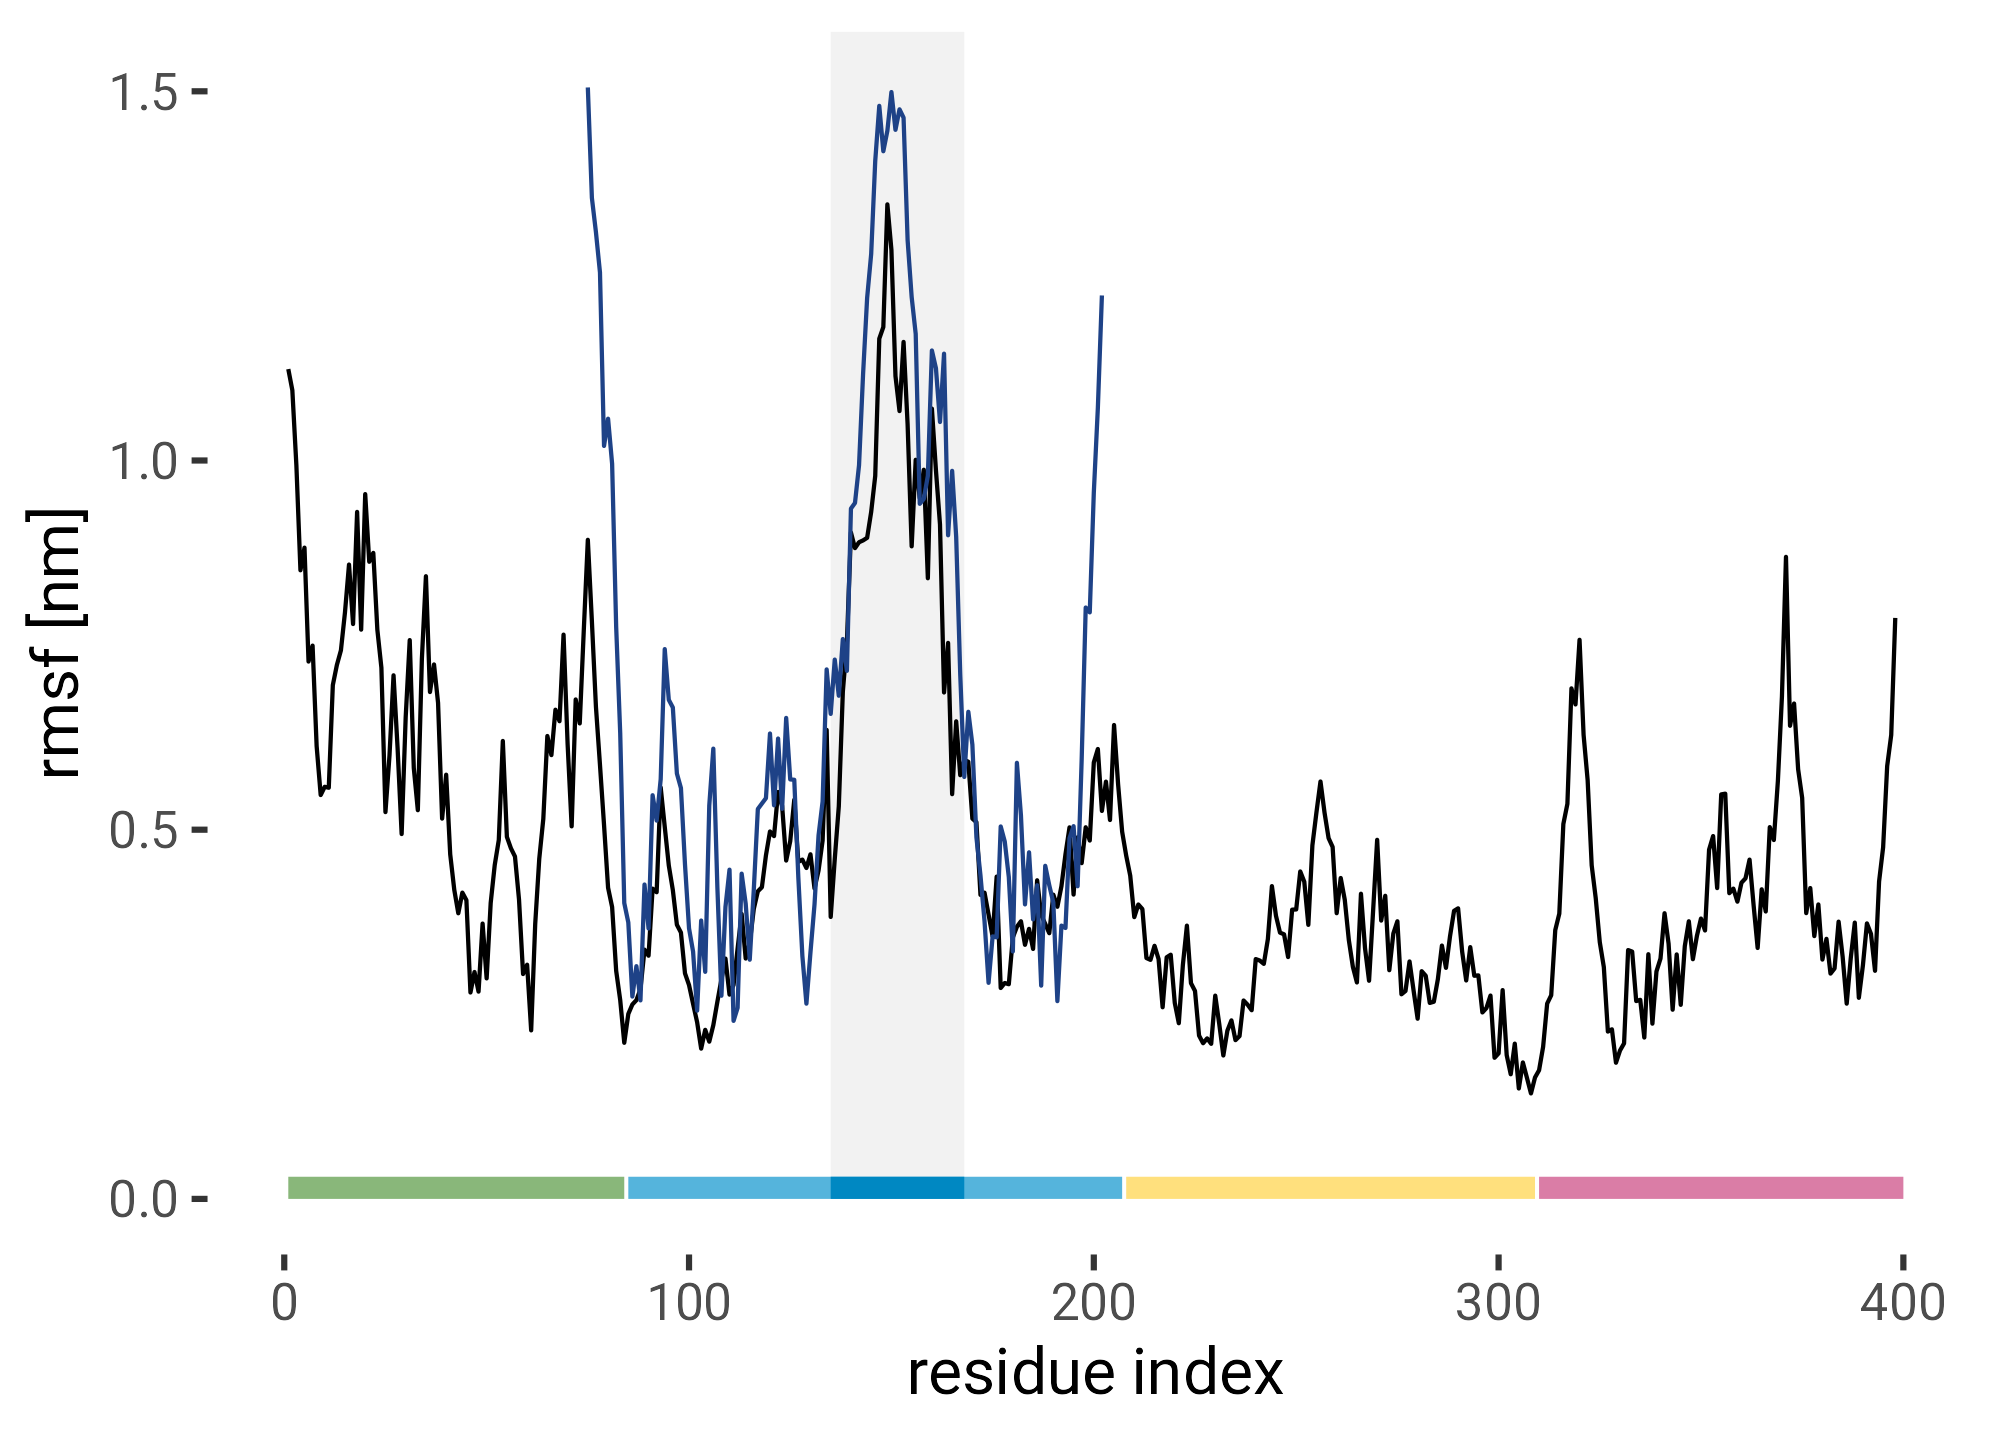
\includegraphics{./results/plots/ferm-rmsf-1.png}

}

}

\subcaption{\label{fig-loop-rmsf}~}
\end{minipage}%
%
\begin{minipage}[t]{0.50\linewidth}

{\centering 

\raisebox{-\height}{

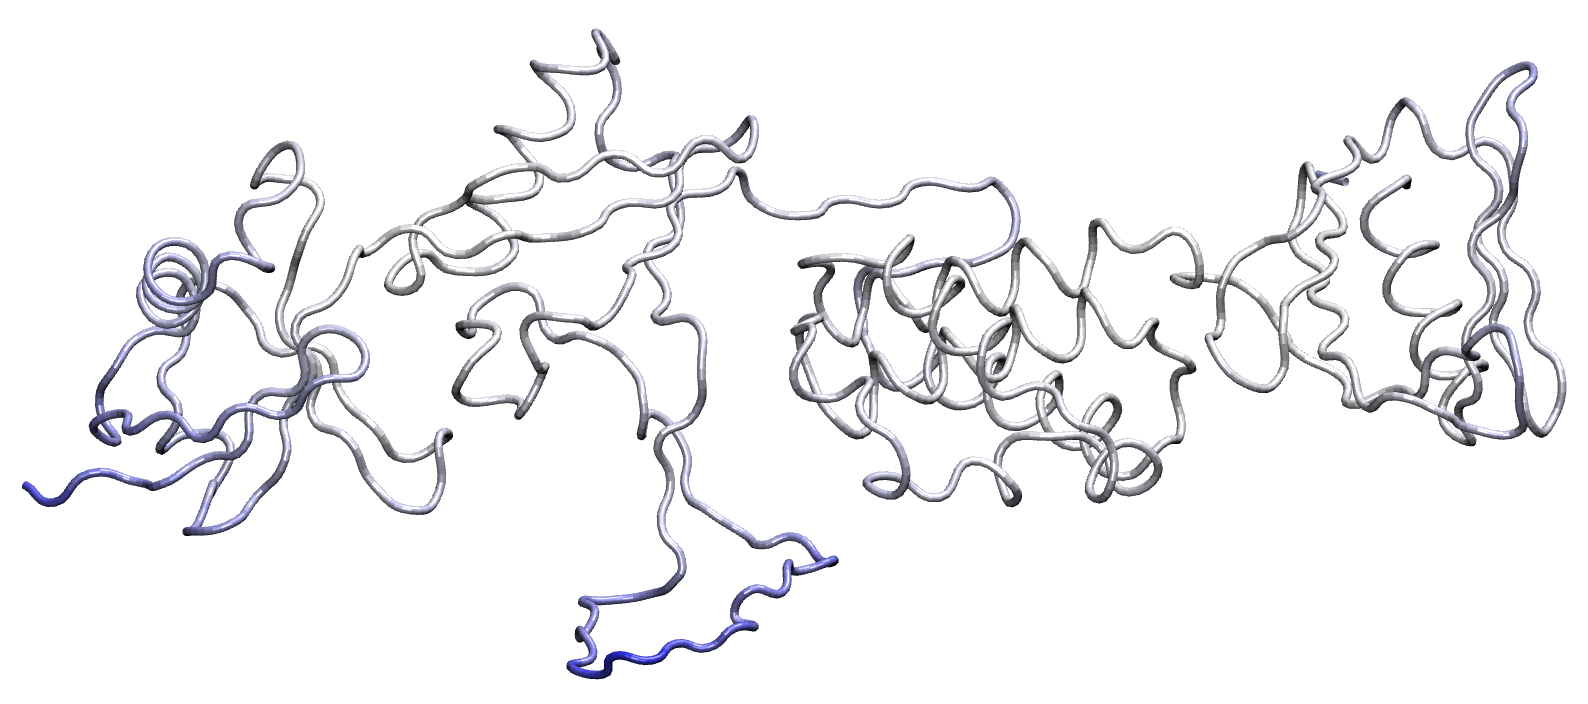
\includegraphics{./assets/results/figures/loop-rmsf-transparent.png}

}

}

\subcaption{\label{fig-loop-rmsf-render}~}
\end{minipage}%
\newline
\begin{minipage}[t]{0.50\linewidth}

{\centering 

\raisebox{-\height}{

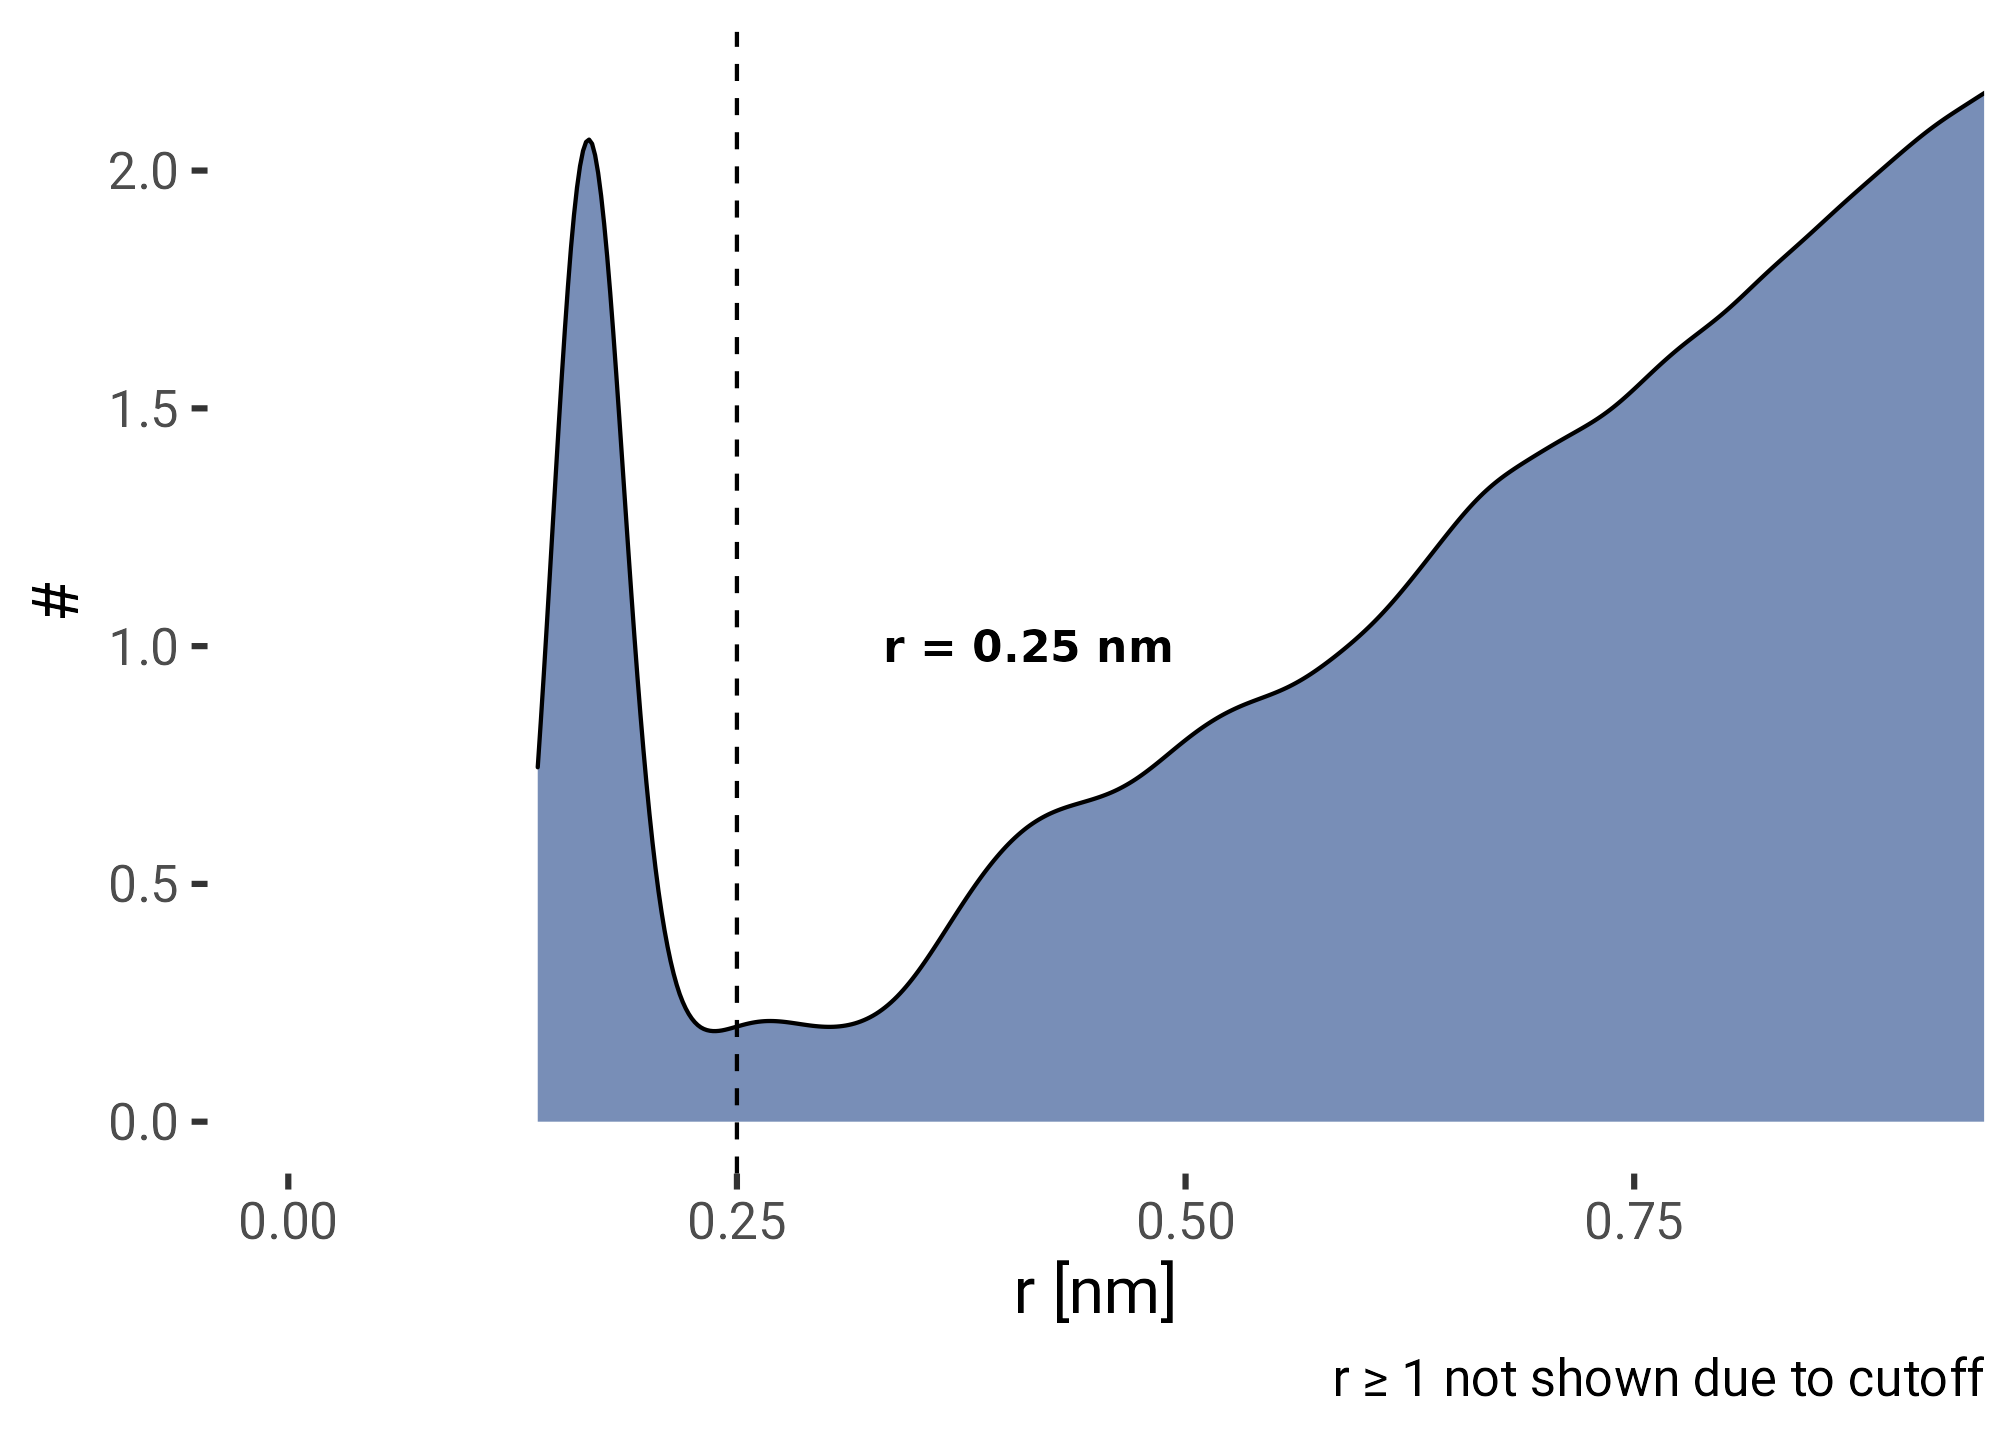
\includegraphics{./results/plots/f0f1-distance-cutoff-1.png}

}

}

\subcaption{\label{fig-r-hist}~}
\end{minipage}%
%
\begin{minipage}[t]{0.50\linewidth}

{\centering 

\raisebox{-\height}{

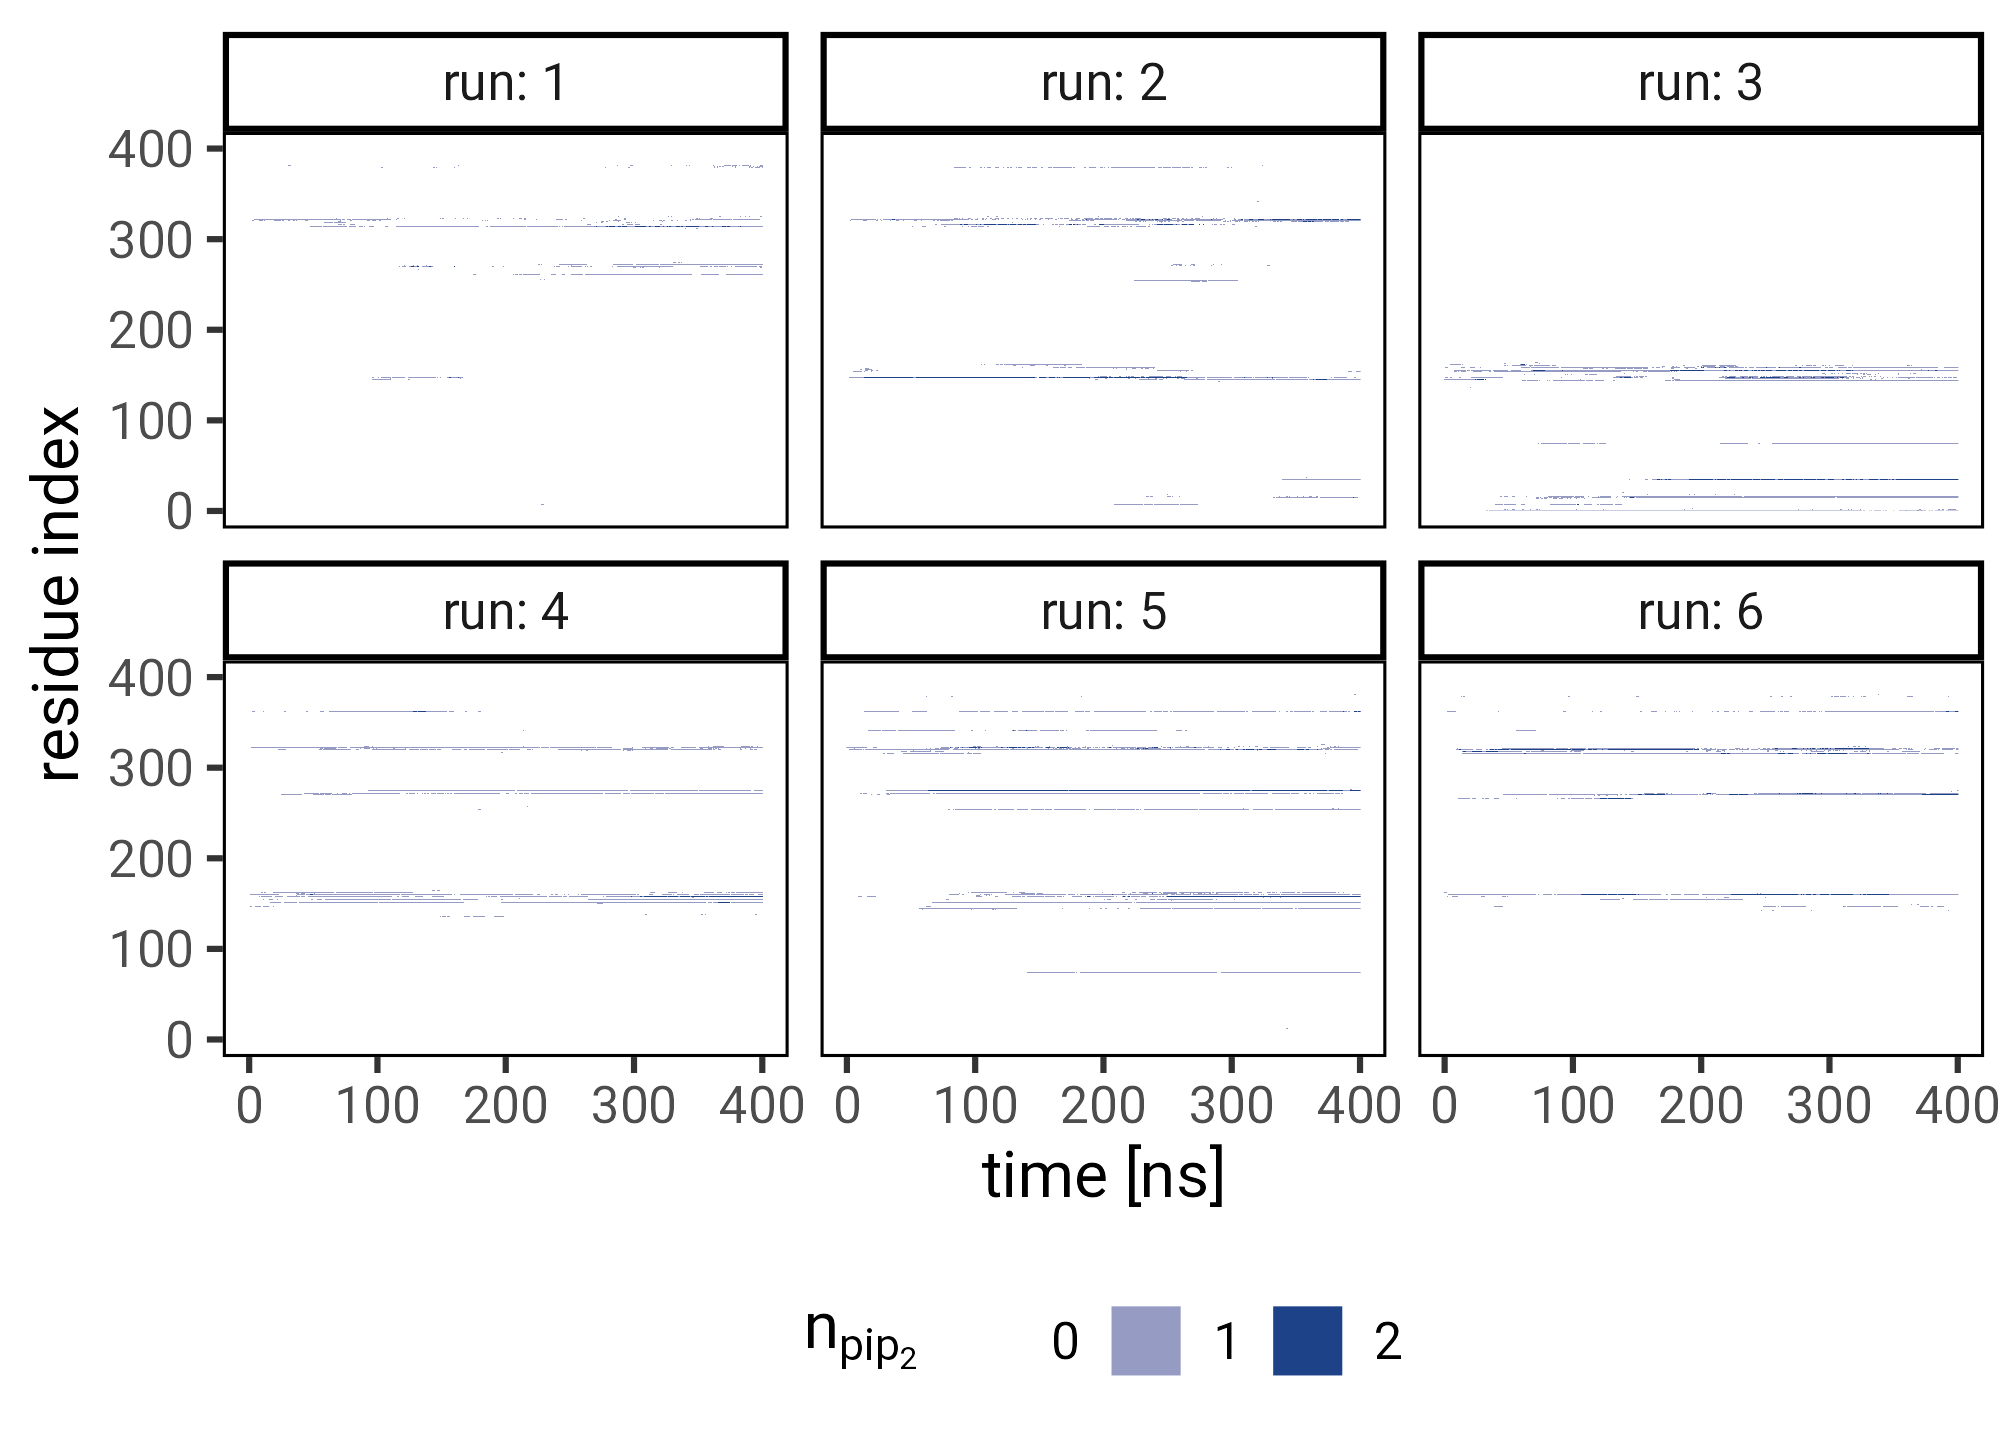
\includegraphics{./results/plots/ferm-time-ri-npip-all-1.png}

}

}

\subcaption{\label{fig-ferm-time-ri-npip-all}~}
\end{minipage}%

\caption{\label{fig-suppl}\textbf{a)} Root Mean Squared Fluctuation
(RMSF) per residue in an equilibrium simulation of the full-length FERM
domain (black). The additional blue line shows the RMSF of the NMR
ensemble of F1 for comparison (2KC2
(\protect\hyperlink{ref-goultStructureDoubleUbiquitinlike2010}{13})).
The region of the loop in F1 is highlighted by a grey shade. Color bars
as in Figure~\ref{fig-ferm-memb-system}. \textbf{b)} The relative
magnitude of the RMSF is shown by coloring the backbone in a render of
the FERM structure. \textbf{c)} Density plot of distances between
PIP\textsubscript{2} and the protein residues to decide on a cutoff for
defining interactions. A distance of 0.25~nm was chosen. \textbf{d)} A
heatmap of the number of PIP\textsubscript{2} molecules bound per
residue over time for the 6 individual simulations with the whole FERM
domain over the membrane.}

\end{figure}

\begin{figure}

\begin{minipage}[t]{0.50\linewidth}

{\centering 

\raisebox{-\height}{

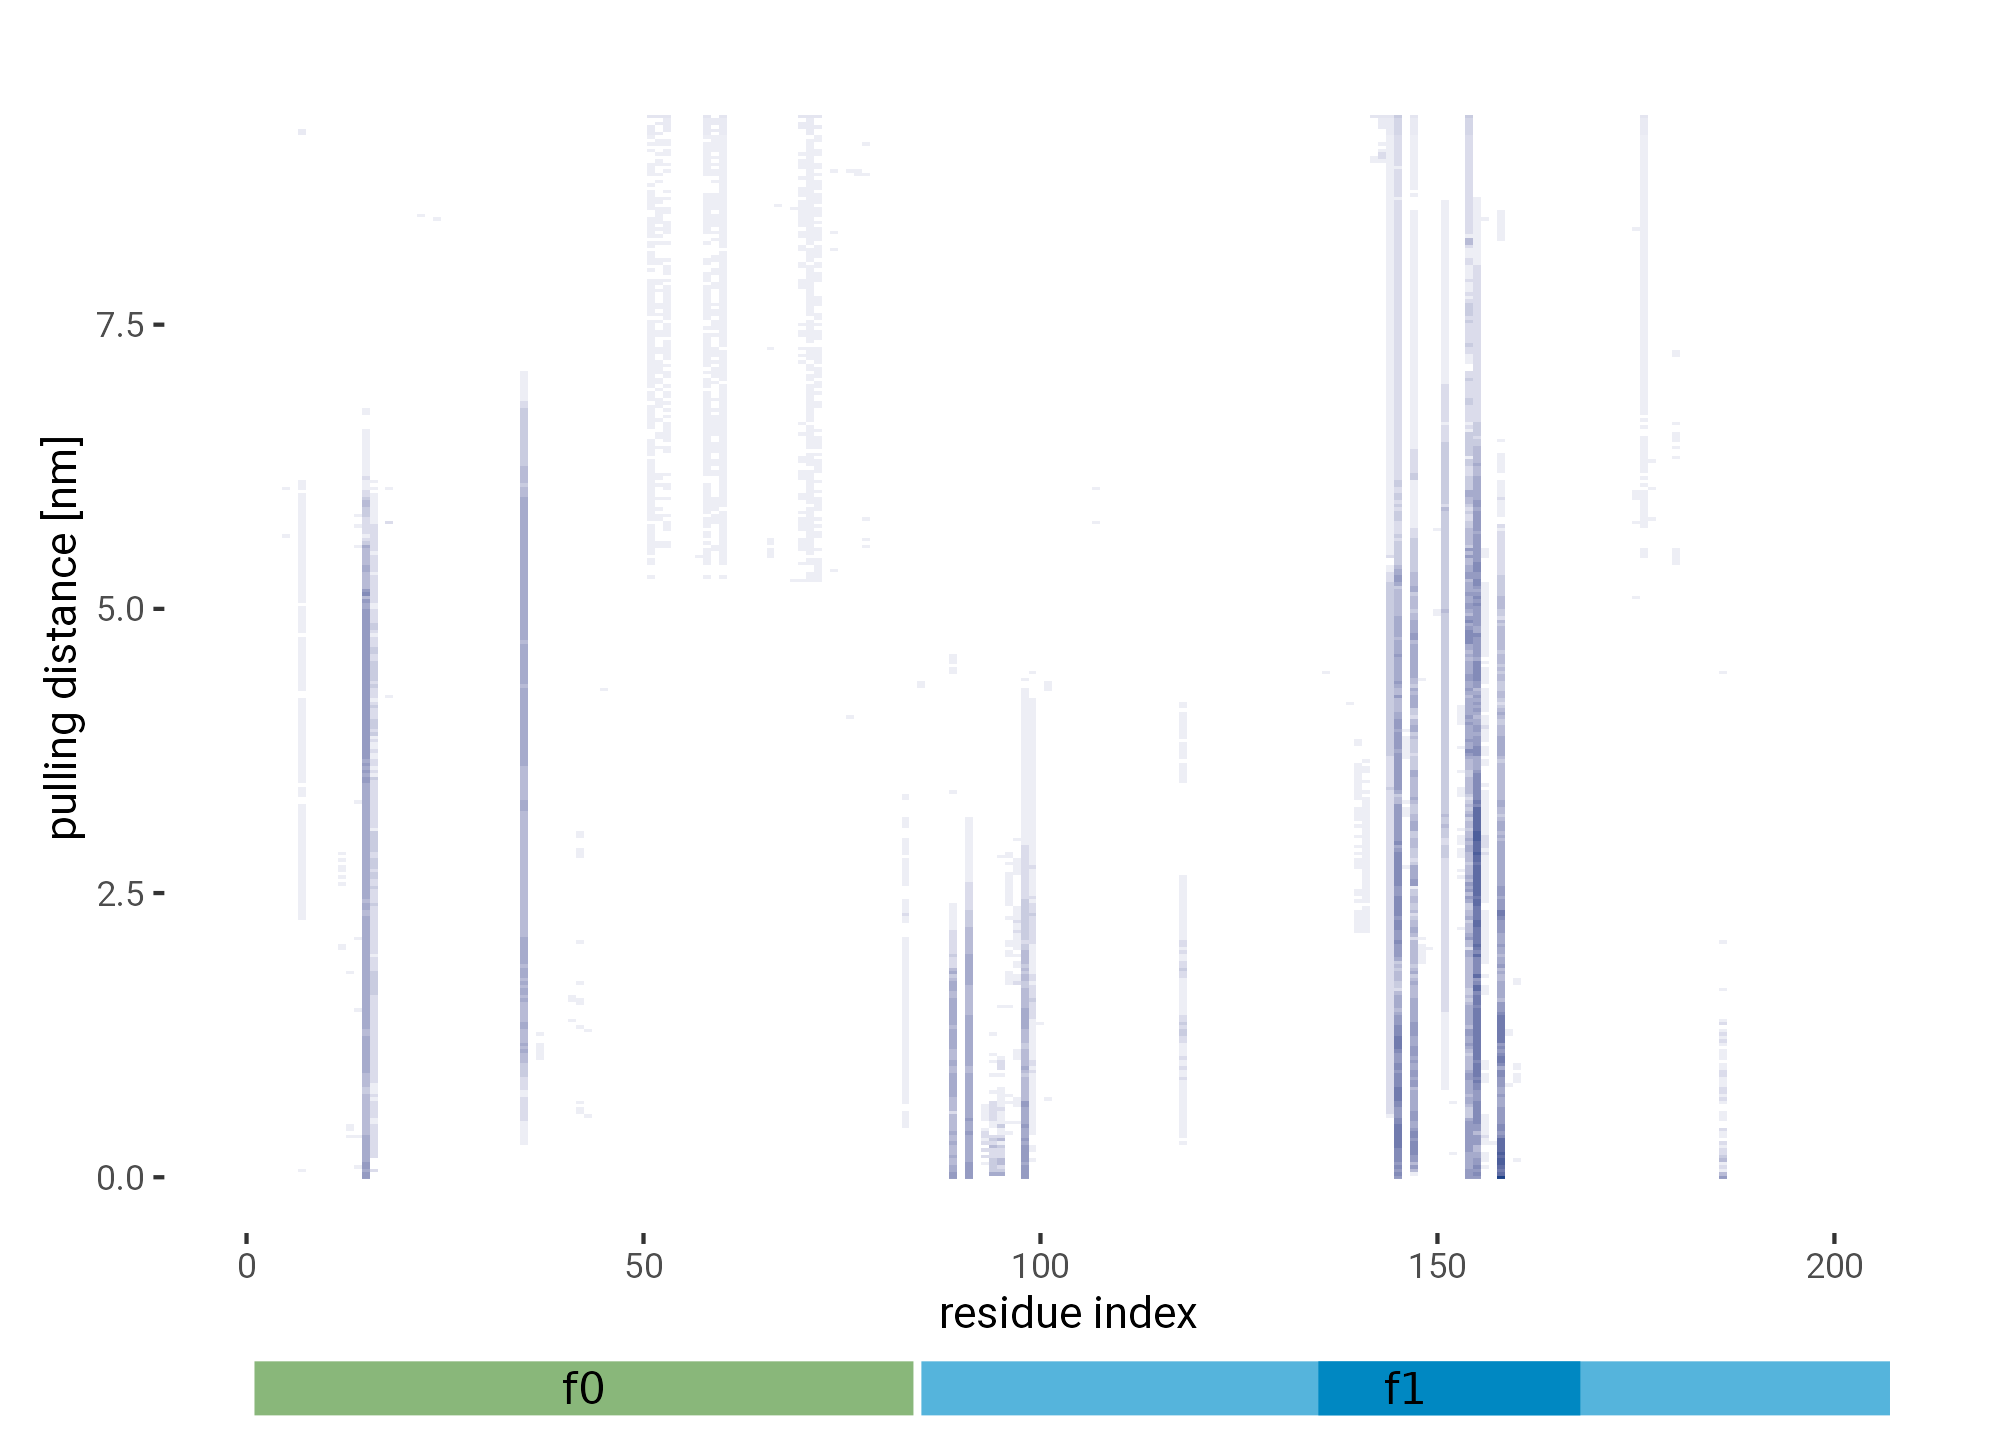
\includegraphics{./results/plots/f0f1-vert-pull-residues-1.png}

}

}

\subcaption{\label{fig-f0f1-vert-pull-residues}~}
\end{minipage}%
%
\begin{minipage}[t]{0.50\linewidth}

{\centering 

\raisebox{-\height}{

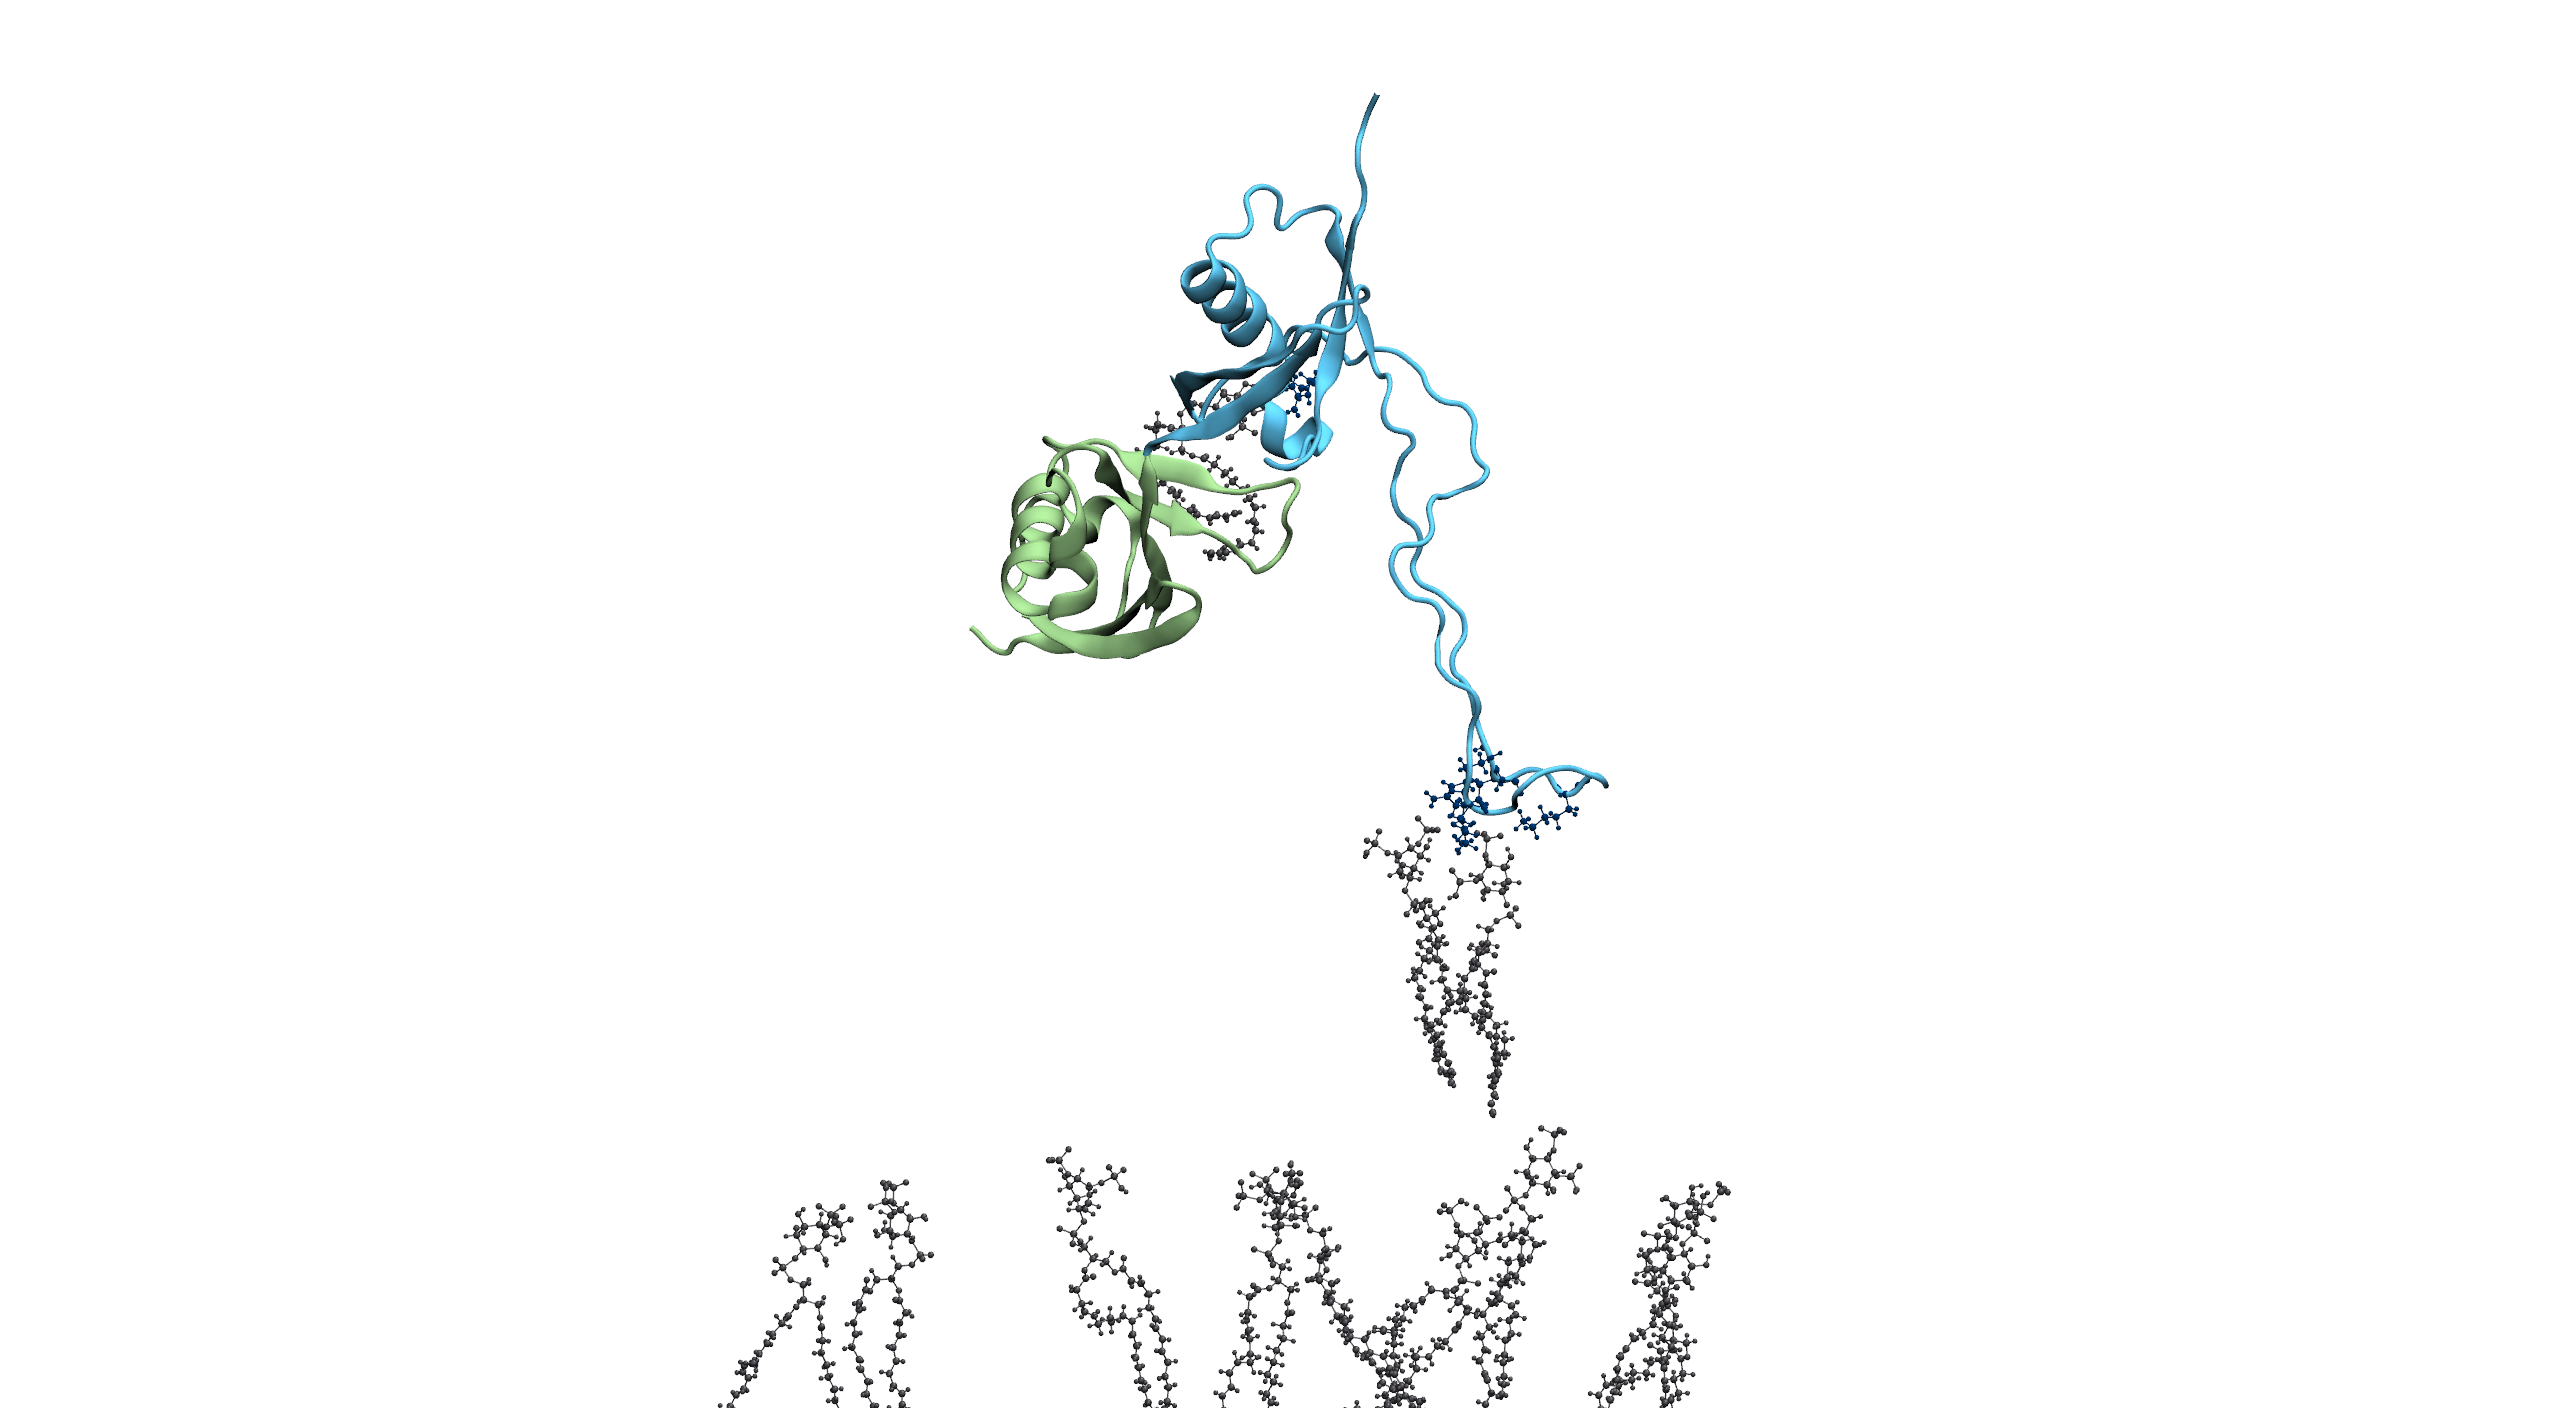
\includegraphics{./assets/vmd/f0f1-pulling/snapshot-run4.png}

}

}

\subcaption{\label{fig-f0f1-vert-pull-run4}~}
\end{minipage}%
\newline
\begin{minipage}[t]{0.50\linewidth}

{\centering 

\raisebox{-\height}{

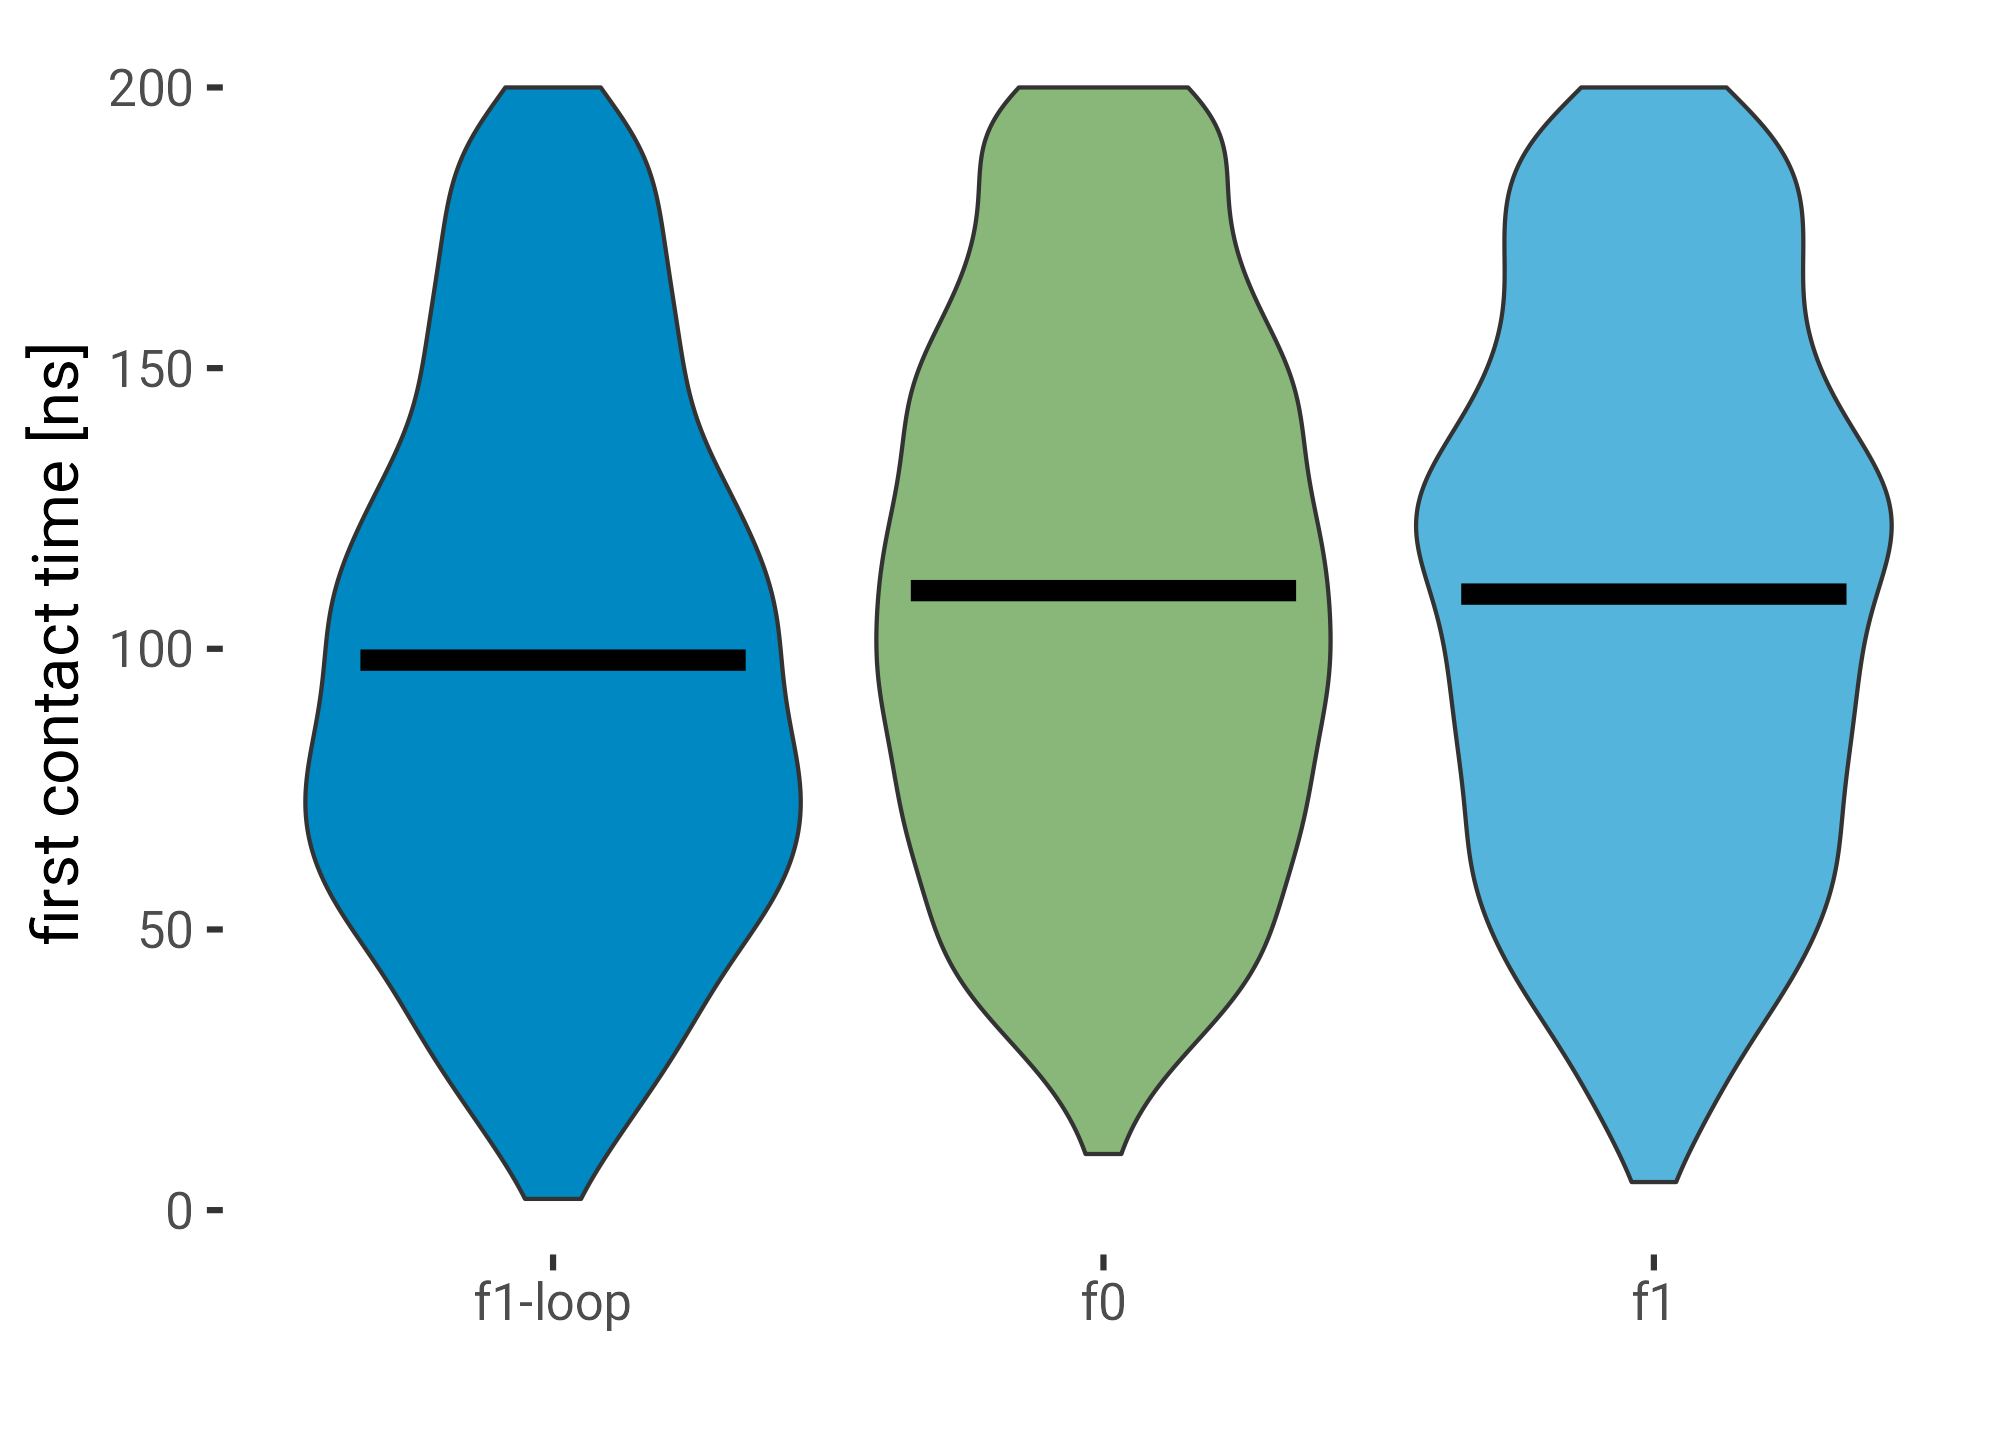
\includegraphics{./results/plots/si-f0f1-first-contact-frame-1.png}

}

}

\subcaption{\label{fig-f0f1-time-to-contact}~}
\end{minipage}%
%
\begin{minipage}[t]{0.50\linewidth}

{\centering 

\raisebox{-\height}{

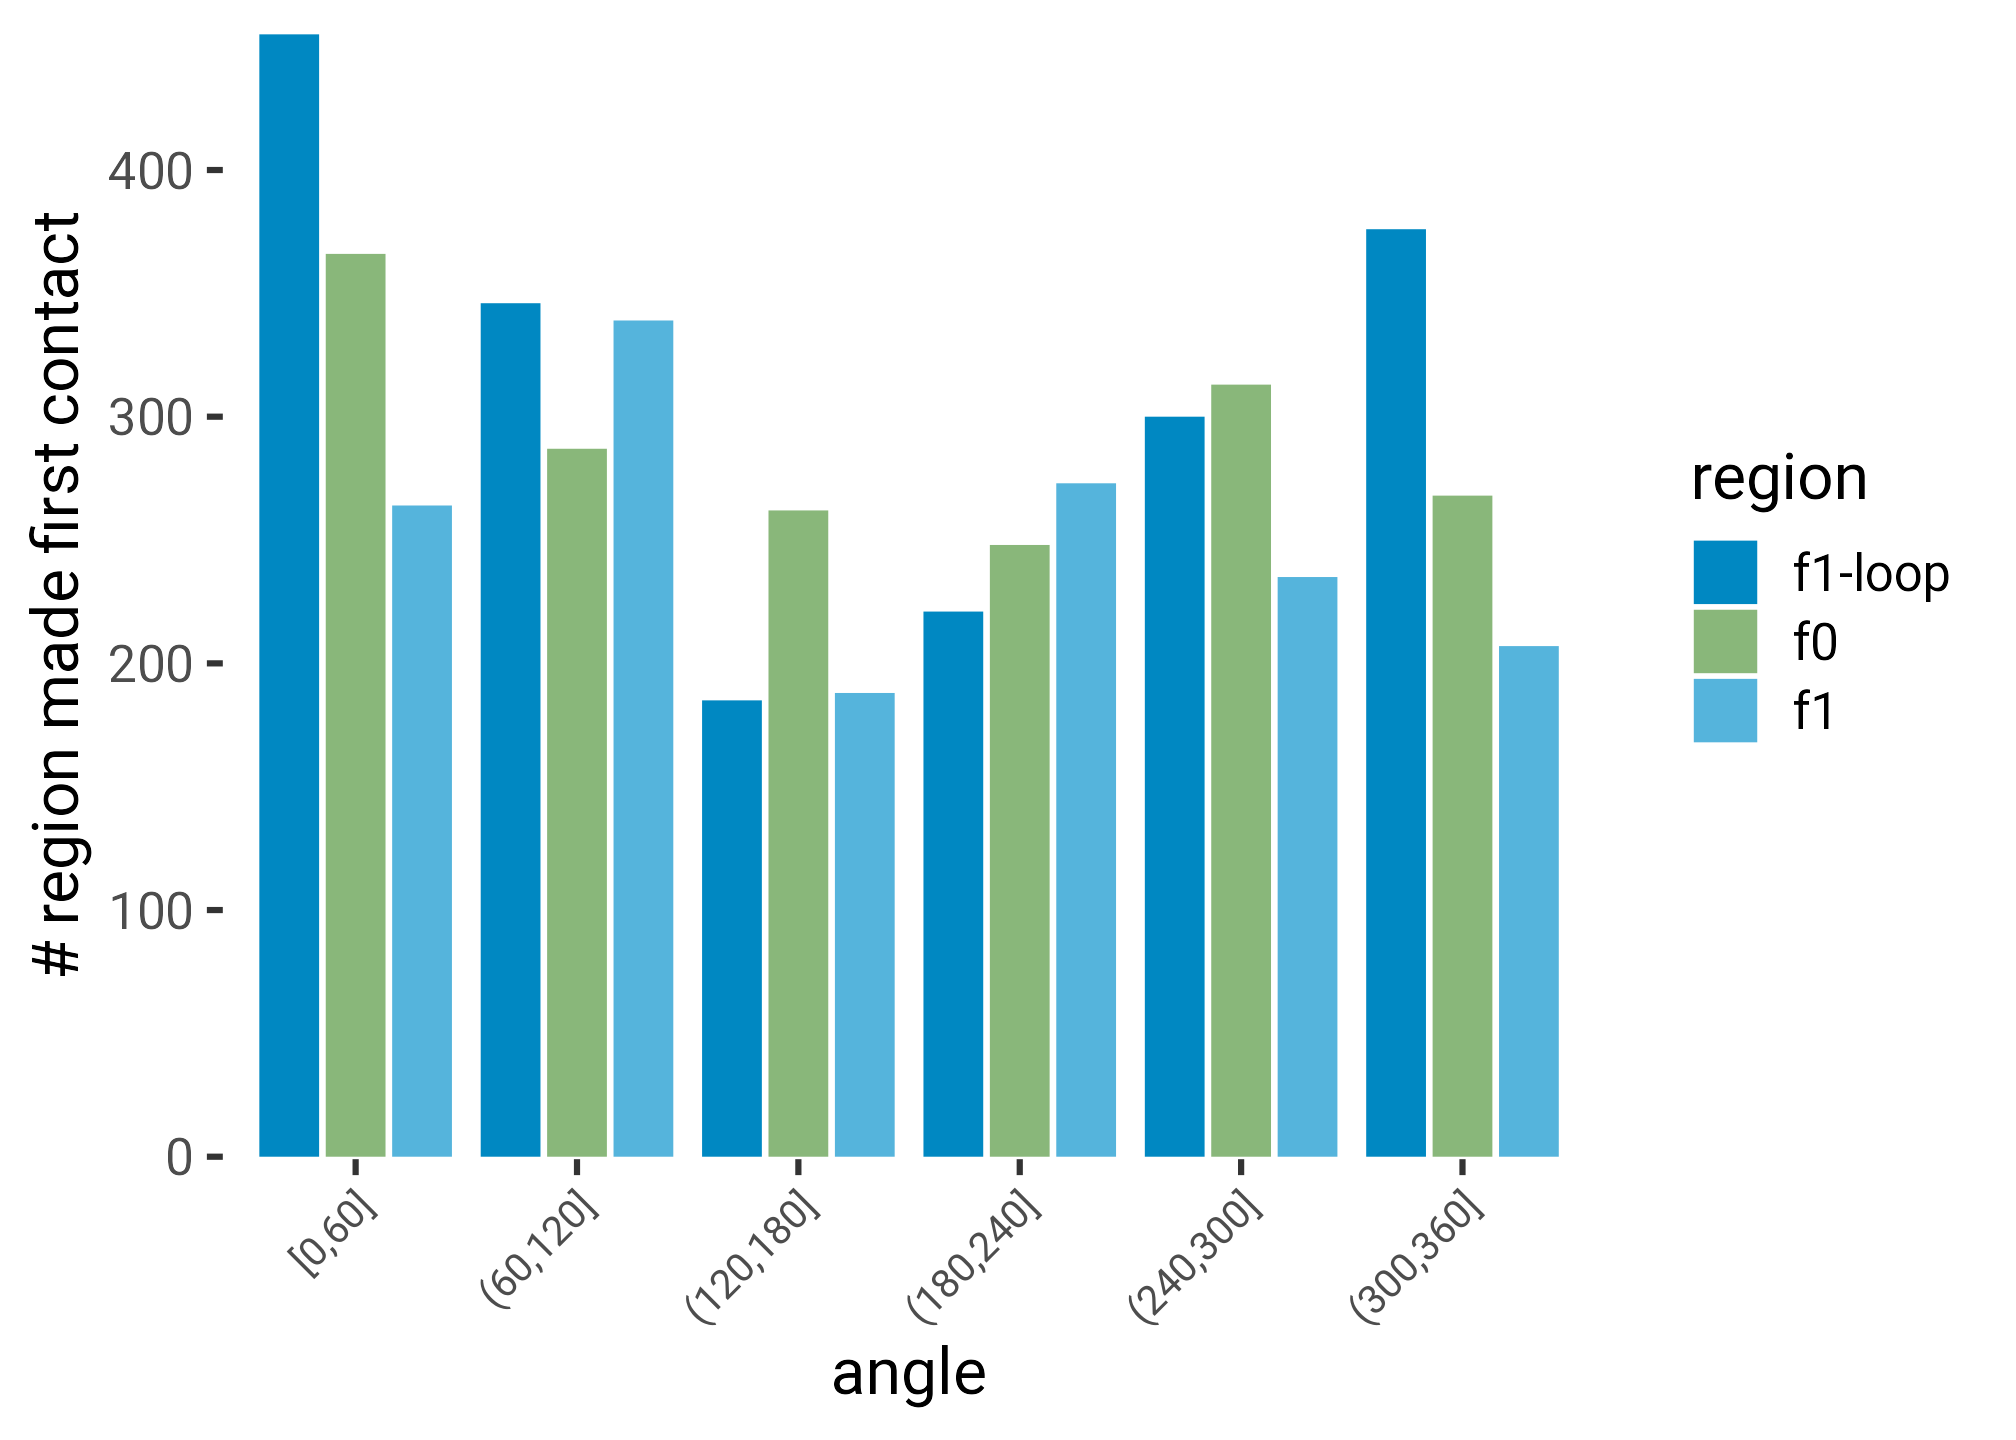
\includegraphics{./results/plots/si-f0f1-angle-first-to-find-1.png}

}

}

\subcaption{\label{fig-f0f1-first-to-find}~}
\end{minipage}%

\caption{\label{fig-suppl-2}\textbf{a)} A closer look at the residues
involved in the interaction during pulling reveals the instrumental role
of both the F1 loop as well as the F0 subdomain in keeping the
connection to the membrane. \textbf{b)} Run 4 of the vertical pulling of
F0F1. Interactions between the protein and PIP\textsubscript{2} were so
strong that a total of 3 molecules of PIP\textsubscript{2} (gray) were
pulled out of the membrane (1 by F0 (green) and 2 by the F1 loop
(blue)). \textbf{c)} Time to first contact of a residue with
PIP\textsubscript{2} in the rotational sampling of F0F1. Residues
belonging to the F1 loop on average make contact earlier. \textbf{d)}
Number of times a residue belonging to a region made the first contact
in the rotational sampling of F0F1.}

\end{figure}

\begin{figure}

\begin{minipage}[t]{0.50\linewidth}

{\centering 

\raisebox{-\height}{

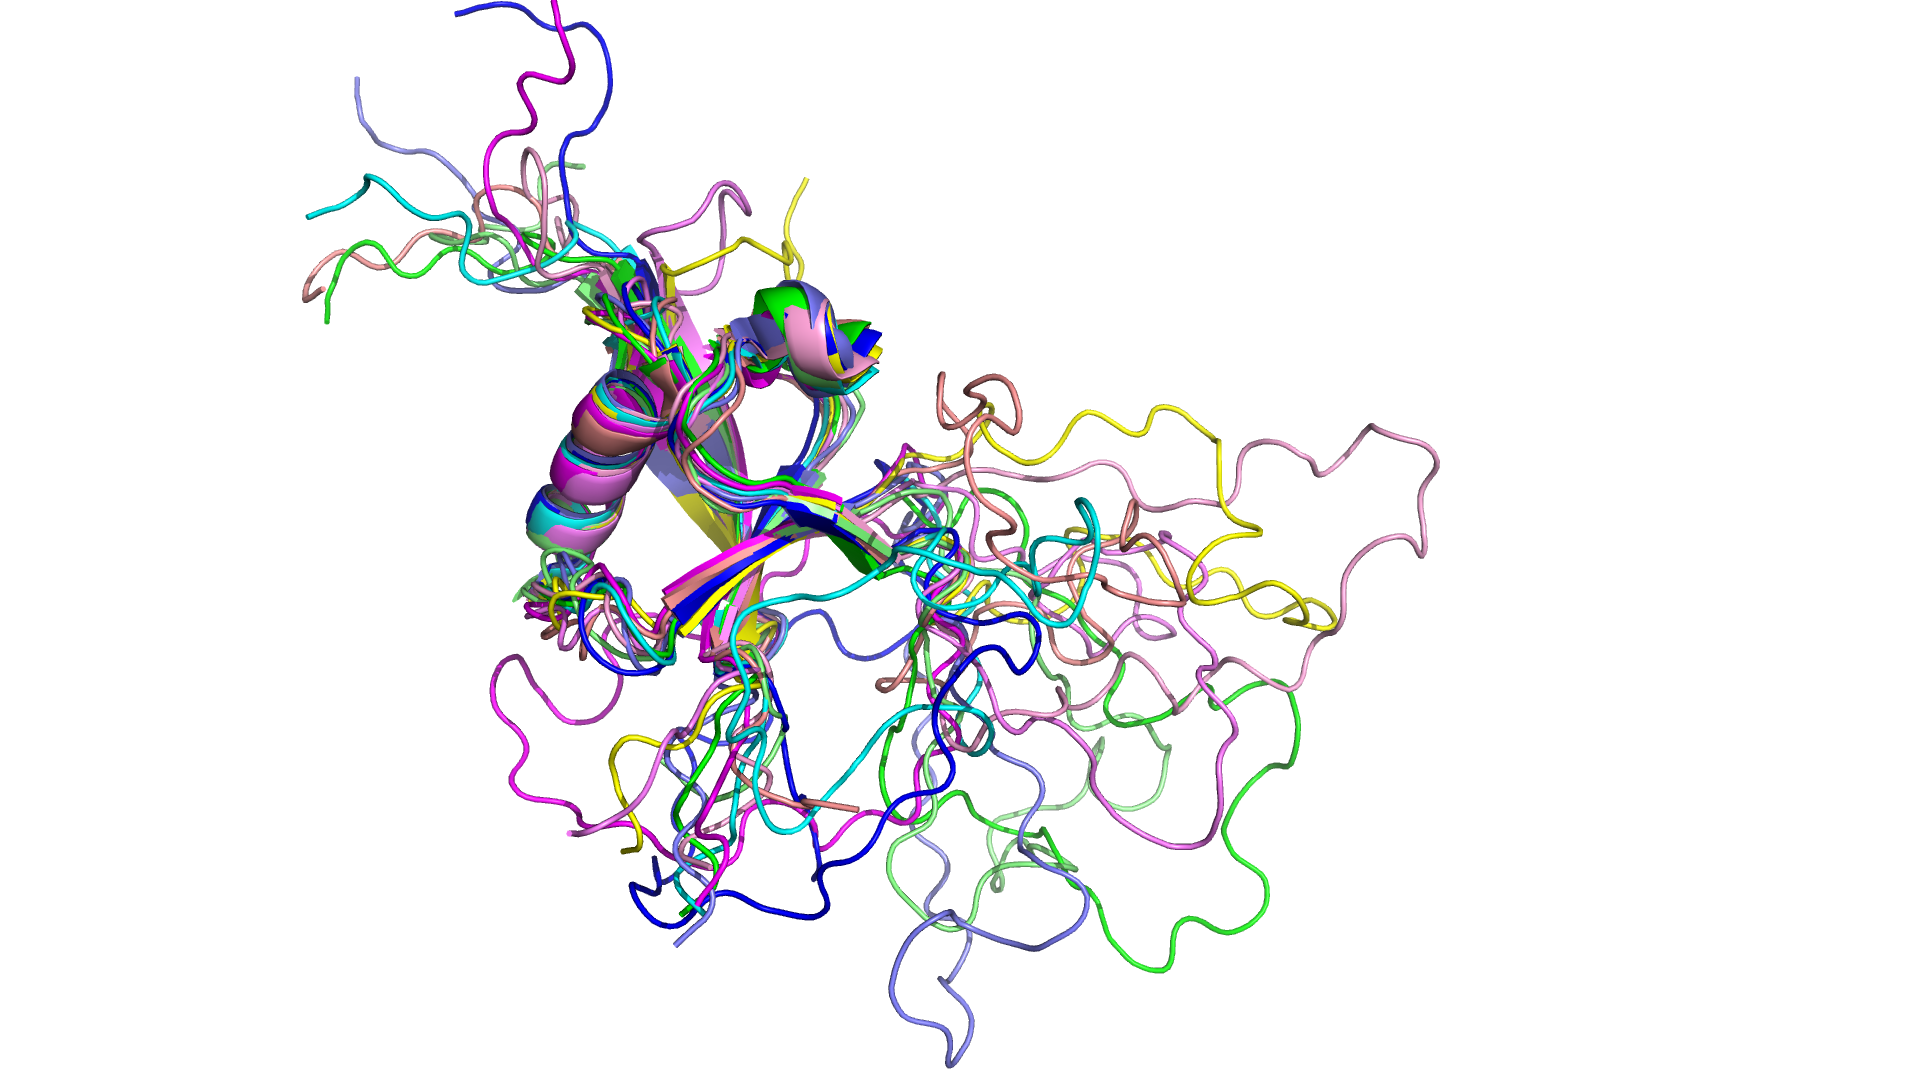
\includegraphics{./assets/structures/2kc2-ensemble-10.png}

}

}

\subcaption{\label{fig-nmr-ensemble}~}
\end{minipage}%
%
\begin{minipage}[t]{0.50\linewidth}

{\centering 

\raisebox{-\height}{

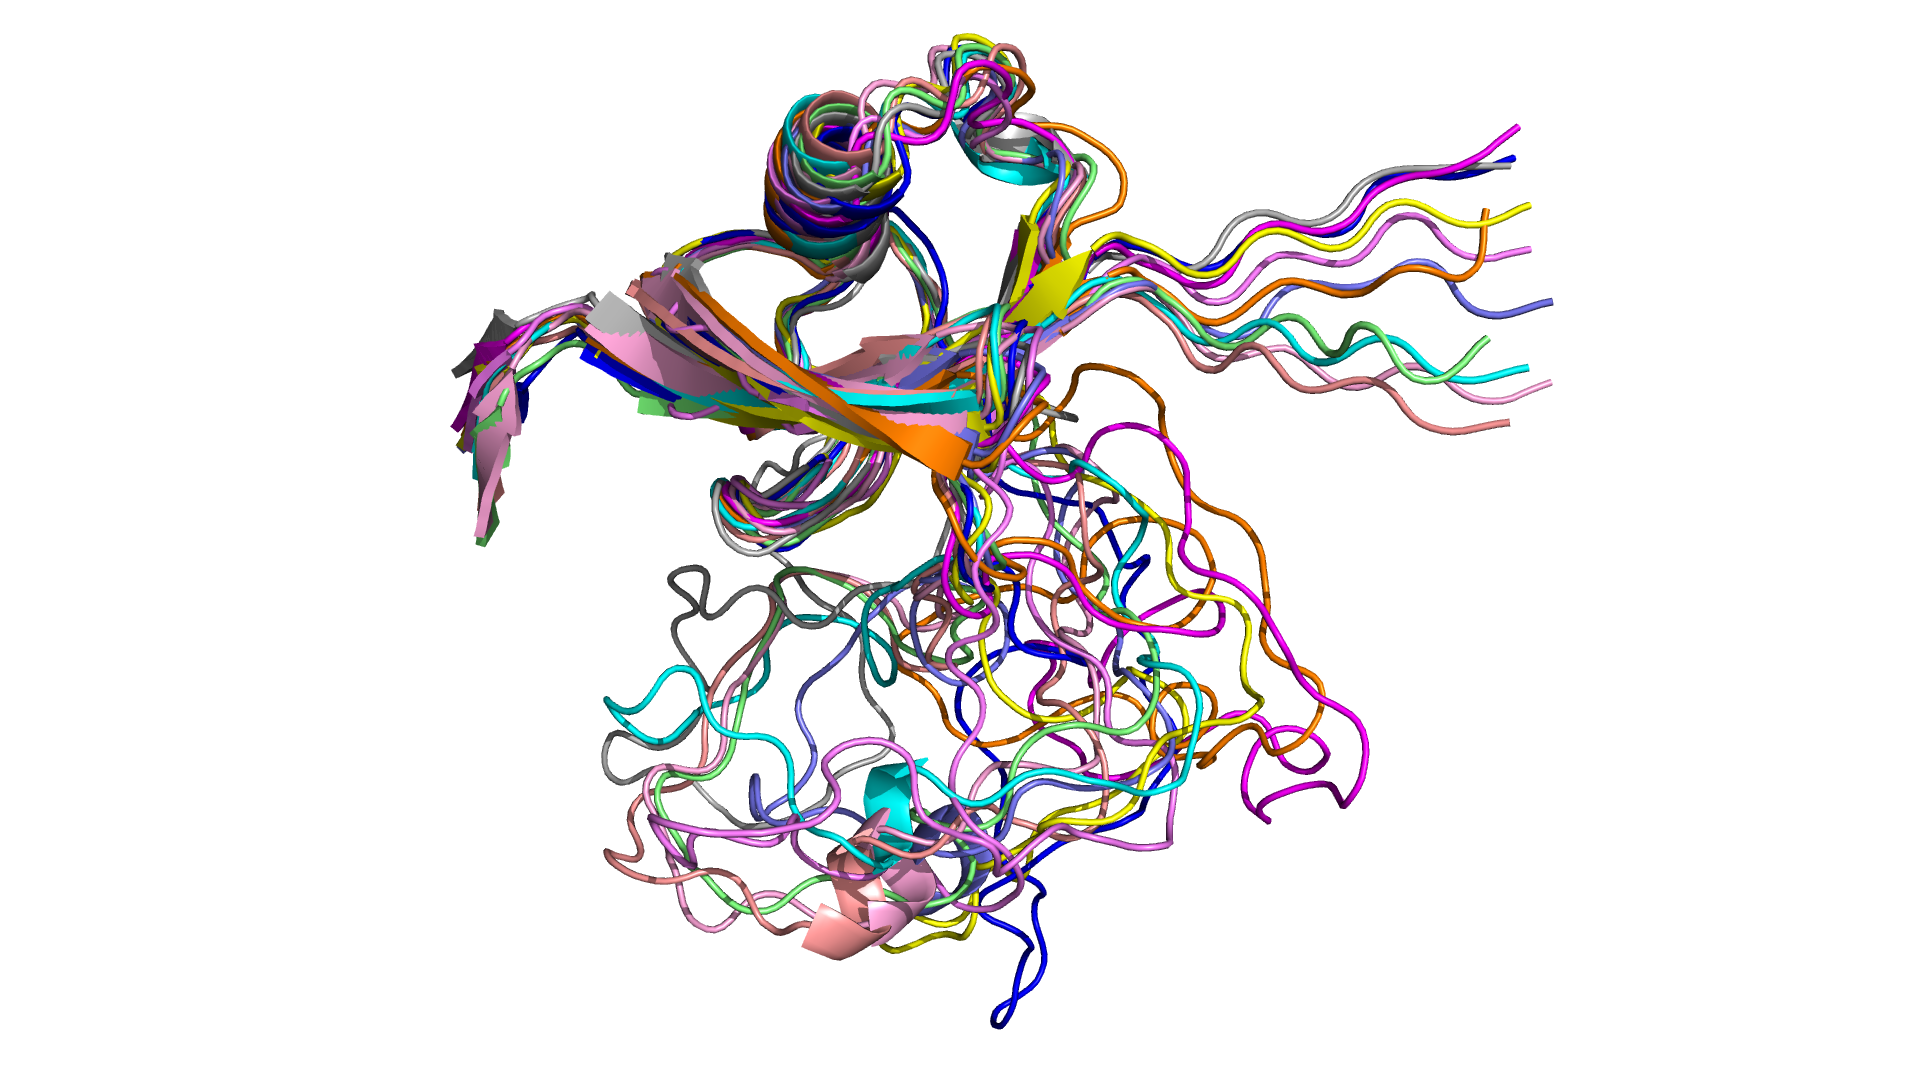
\includegraphics{./assets/structures/ferm-eq-ensemble-10.png}

}

}

\subcaption{\label{fig-ferm-ensemble}~}
\end{minipage}%

\caption{\label{fig-suppl-3}\textbf{a)} NMR ensemble of F1, pdb ID 2KC2
(\protect\hyperlink{ref-goultStructureDoubleUbiquitinlike2010}{13})
\textbf{b)} Ensemble of the F1 domain in equilibrium simulations of the
completed FERM domain. The other domains (F0,F2,F3) are not shown, but
their steric influence can be seen, as the flexible loop can now no
longer occupy the space of the F2 domain as in the NMR structure in
\textbf{a}.}

\end{figure}

\twocolumn

\hypertarget{tbl-f0f1-top-interacting}{}
\begin{longtable}[]{@{}lr@{}}
\caption{\label{tbl-f0f1-top-interacting}Top residues interacting with
F0F1}\tabularnewline
\toprule()
residue & mean\_n\_pip \\
\midrule()
\endfirsthead
\toprule()
residue & mean\_n\_pip \\
\midrule()
\endhead
M 1 & 0.118 \\
K 15 & 0.114 \\
R 30 & 0.104 \\
R 35 & 0.155 \\
K 98 & 0.101 \\
R 118 & 0.127 \\
R 144 & 0.179 \\
K 147 & 0.155 \\
R 151 & 0.209 \\
K 154 & 0.144 \\
K 155 & 0.152 \\
K 158 & 0.154 \\
K 160 & 0.139 \\
K 162 & 0.107 \\
R 193 & 0.120 \\
\bottomrule()
\end{longtable}

\hypertarget{tbl-ferm-top-interacting}{}
\begin{longtable}[]{@{}lr@{}}
\caption{\label{tbl-ferm-top-interacting}Top residues interacting with
FERM}\tabularnewline
\toprule()
residue & mean\_n\_pip \\
\midrule()
\endfirsthead
\toprule()
residue & mean\_n\_pip \\
\midrule()
\endhead
M 1 & 0.144 \\
K 15 & 0.154 \\
T 16 & 0.134 \\
R 35 & 0.202 \\
R 74 & 0.195 \\
R 144 & 0.555 \\
K 145 & 0.199 \\
K 147 & 0.426 \\
R 151 & 0.295 \\
K 154 & 0.149 \\
K 155 & 0.391 \\
K 158 & 0.506 \\
K 160 & 0.679 \\
K 162 & 0.174 \\
K 254 & 0.157 \\
K 270 & 0.242 \\
K 272 & 0.412 \\
R 275 & 0.416 \\
K 314 & 0.281 \\
K 316 & 0.310 \\
K 320 & 0.742 \\
N 321 & 0.298 \\
K 322 & 0.507 \\
K 341 & 0.248 \\
K 362 & 0.447 \\
\bottomrule()
\end{longtable}

\newpage
\clearpage

\hypertarget{molecular-dynamics-parameters}{%
\subsection{Molecular dynamics
Parameters}\label{molecular-dynamics-parameters}}

\hypertarget{sec-prod-mdp}{%
\subsubsection{Production runs}\label{sec-prod-mdp}}

\begin{verbatim}
integrator              = md
dt                      = 0.002
nsteps                  = 100000000
cutoff-scheme           = Verlet
nstlist                 = 20
rlist                   = 1.2
coulombtype             = pme
rcoulomb                = 1.2
vdwtype                 = Cut-off
vdw-modifier            = Force-switch
rvdw_switch             = 1.0
rvdw                    = 1.2
tcoupl                  = Nose-Hoover
tc_grps                 = SYSTEM
tau_t                   = 1.0
ref_t                   = 303.15
pcoupl                  = Parrinello-Rahman
pcoupltype              = semiisotropic
tau_p                   = 5.0
compressibility         = 4.5e-5  4.5e-5
ref_p                   = 1.0     1.0
constraints             = h-bonds
constraint_algorithm    = LINCS
continuation            = yes
nstcomm                 = 100
comm_mode               = linear
comm_grps               = SYSTEM
refcoord_scaling        = com
\end{verbatim}



\end{document}
